\documentclass[10pt]{book}

% Be sure to use PDF Latex
\pdfoutput=1

% links
\usepackage[bookmarks,bookmarksdepth=2, colorlinks=true, linkcolor=blue,citecolor=red, urlcolor=blue]{hyperref}



\usepackage{fullpage}

\usepackage[latin1]{inputenc}
\usepackage{mystyle}
\usepackage{wrapfig}
\usepackage{notations_ot} % for OT chapter
\usepackage{pdfpages} % to include multiple pages pdf

\graphicspath{{./figures/}{./figures/ot/}}


\newcommand{\myauthor}[3]{#1\protect\footnote{#2, \protect\url{#3}}}


\title{\Huge \sf Mathematical Foundations of Data Sciences\vspace{1cm}
\includegraphics[width=.9\linewidth]{wave}} 

\author{%
\begin{tabular}{c}
	Gabriel Peyr{\'e} \\ CNRS \& DMA \\
	 \'Ecole Normale Sup\'erieure \\
	 \url{gabriel.peyre@ens.fr}\\
	 \url{https://mathematical-tours.github.io}\\
	 \url{www.numerical-tours.com}
\end{tabular}
}


\date{\today}

%%

\begin{document}

\maketitle

%% !TEX root = ../FundationsDataScience.tex

\chapter*{Presentation}

% \begin{abstract}
	This book draft presents an overview of important mathematical and numerical foundations for modern data sciences. 
	% 
	It covers in particulars the basics of signal and image processing (Fourier, Wavelets, and their applications to denoising and compression), imaging sciences (inverse problems, sparsity, compressed sensing) and machine learning (linear regression, logistic classification, deep learning). 
	%
	The focus is on the mathematically-sounded exposition of the methodological tools (in particular linear operators, non-linear approximation, convex optimization, optimal transport) and how they can be mapped to efficient computational algorithms. 
	%
	These course notes are also intended to be the theortical companion for the Numerical Tours\footnote{\url{www.numerical-tours.com}} web site, which presents Matlab/Python/Julia/R detailed implementations of all the concepts covered here.
		
% \end{abstract}

\tableofcontents




%
%% !TEX root = ../FundationsDataScience.tex

\chapter{Shannon Theory}
\label{sec-shannon}

%
Shannon theory of information, published in 1948/1949, is made of three parts:
\begin{enumerate}
	\item Sampling: it studies condition under which sampling a continuous function to obtain a discrete vector is invertible. The discrete real values representing the signal are then typically quantized to a finite precision to obtain a set of symbols in a finite alphabet.  
	\item Source coding: it studies optimal ways to represent (code) such a set of symbols as a binary sequence. It leverages the statistical distributions to obtain the most possible compact code.  
	\item Channel coding (not studied here): it studies how to add some redundancy to the coded sequence in order to gain robustness to errors or attacks during transmission (flip of certain bits with some probability). It is often named ``error correcting codes theory''. 
\end{enumerate}
%
The main reference for this chapter is~\cite{mallat2008wavelet}.


%%%%%%%%%%%%%%%%%%%%%%%%%%%%%%%%%%%%%%%%%%%%%%%%%%%%%%%%%%%%%%%%%%%%
%%%%%%%%%%%%%%%%%%%%%%%%%%%%%%%%%%%%%%%%%%%%%%%%%%%%%%%%%%%%%%%%%%%%
%%%%%%%%%%%%%%%%%%%%%%%%%%%%%%%%%%%%%%%%%%%%%%%%%%%%%%%%%%%%%%%%%%%%
\section{Analog vs. Discrete Signals}

To develop numerical tools and analyze their performances, the mathematical modelling is usually done over a continuous setting (so-called ``analog signals''). 
%
Such continuous setting also aims at representing the signal in the physical world, which are inputs to sensors hardwares such as microphone, digital cameras or medical imaging devices. 
%
An analog signal is a 1-D function $f_0 \in \Ldeux([0,1])$ where $[0,1]$ denotes the domain of acquisition, which might for instance be time. An analog image is a 2D function $f_0 \in \Ldeux([0,1]^2)$ where the unit square $[0,1]^2$ is the image domain.

Although these notes are focussed on the processing of sounds and natural images, most of the methods extend to multi-dimensional datasets, which are higher dimensional mappings
\eq{
	f_0 : [0,1]^d \rightarrow [0,1]^s
}
where $d$ is the dimensionality of the input space ($d=1$ for sound and $d=2$ for images) whereas $s$ is the dimensionality of the feature space. For instance, gray scale images corresponds to $(d=2,s=1)$, 
videos to $(d=3, s=1)$, color images to $(d=2, s=3)$ where one has three channels $(R,G,B)$.
One can even consider multi-spectral images where $(d=2, s \gg 3)$ that is made of a large number of channels for different light wavelengths. Figures \ref{fig-examples-1} and \ref{fig-examples-2} show examples of such data.


\myfigure{
	\image{orthobases}{.35}{example-sound}
	\image{orthobases}{.28}{example-image}
	\image{orthobases}{.3}{example-video}
}{%
	Examples of sounds ($d=1$), image ($d=2$) and videos ($d=3$). %	
}{fig-examples-1}

\myfigure{
	\image{orthobases}{.4}{example-color}
	\image{orthobases}{.5}{example-multispectral}
}{%
	Example of color image $s=3$ and multispectral image ($s=32$). %	
}{fig-examples-2}


%%%%%%%%%%%%%%%%%%%%%%%%%%%%%%%%%%%%%%%%%%%
\subsection{Acquisition and Sampling}

Signal acquisition is a low dimensional projection of the continuous signal performed by some hardware device. This is for instance the case for a microphone that acquires 1D samples or a digital camera that acquires 2D pixel samples.
The sampling operation thus corresponds to mapping from the set of continuous functions to a discrete finite dimensional vector with $N$ entries.
\eq{
	f_0 \in \Ldeux([0,1]^d) \mapsto f \in \CC^N
}

\myfigure{
	\image{orthobases}{.4}{discretization-image}
	\image{orthobases}{.5}{discretization-sound}
}{%
	Image and sound discretization. %	
}{fig-discretization}

Figure \ref{fig-discretization} shows examples of discretized signals.

%%%%%%%%%%%%%%%%%%%%%%%%%%%%%%%%%%%%%%%%%%%
\subsection{Linear Translation Invariant Sampler}

A translation invariant sampler performs the acquisition as an inner product between the continuous signal and a constant impulse response $h$ translated at the sample location
\eql{\label{eq-linear-sampling}
	f_n = \int_{-S/2}^{S/2} f_0(x) h(n/N - x) \d x= f_0 \star h(n/N).
}
The precise shape of $h(x)$ depends on the sampling device, and is usually a smooth low pass function that is maximal around $x=0$. The size $S$ of the sampler determines the precision of the sampling device, and is usually of the order of $1/N$ to avoid blurring (if $S$ is too large) or aliasing (if $S$ is too small).

Section \ref{sec-sampling} details how to reverse the sampling operation in the case where the function is smooth.


%%%%%%%%%%%%%%%%%%%%%%%%%%%%%%%%%%%%%%%%%%%%%%%%%%%%%%%%%%%%%%%%%%%%
%%%%%%%%%%%%%%%%%%%%%%%%%%%%%%%%%%%%%%%%%%%%%%%%%%%%%%%%%%%%%%%%%%%%
%%%%%%%%%%%%%%%%%%%%%%%%%%%%%%%%%%%%%%%%%%%%%%%%%%%%%%%%%%%%%%%%%%%%
\section{Shannon Sampling Theorem}
\label{subsec-sampling}

%%%
\paragraph{Reminders about Fourier transform.}

For $f \in L^1(\RR)$, its Fourier transform is defined as
\eql{\label{eq-fourier-transform}
	\foralls \om \in \RR, \quad
	\hat f(\om) \eqdef \int_\RR f(x) e^{-\imath x \om} \d x.
}
One has $\norm{\hat f}^2 = (2\pi)^{-1} \norm{f}^2$, so that $f \mapsto \hat f$ can be extended by continuity to $L^2(\RR)$, which corresponds to computing $\hat f$ as a limit when $T \rightarrow +\infty$ of $\int_{-T}^T f(x) e^{-\imath x \om} \d x$.
%
When $\hat f \in L^1(\RR)$, one can invert the Fourier transform so that
\eql{\label{eq-i-ft}
	f(x) = \frac{1}{2\pi} \int_\RR \hat f(\om) e^{\imath x \om} \d \om, 
}
which shows in particular that $f$ is continuous with vanishing limits at $\pm\infty$. 

The Fourier transform $\Ff : f \mapsto \hat f$ exchanges regularity and decay. For instance, if $f \in C^p(\RR)$ with an integrable Fourier transform, then $\Ff(f^{(p)})(\om) = (\imath \om)^{p} \hat f(\om)$ so that $|\hat f(\om)|=O(1/|\om|^p)$. 
%
Conversely, 
\eql{\label{eq-fourier-regul}
	\int_\RR (1+|\om|)^{p} |\hat f(\om)| \d \om<+\infty
	\qarrq f \in C^p(\RR).
}
For instance, if $\hat f(\om)=O(1/|\om|^{p+2})$, one obtains that $f \in C^p(\RR)$. 

%%%
\paragraph{Reminders about Fourier series.}

We denote $\TT=\RR/2\pi\ZZ$ the torus.
%
A function $f \in L^2(\TT)$ is $2\pi$-periodic, and can be viewed as a function $f \in L^2([0,2\pi])$ (beware that this means that the boundary points are glued together), and its Fourier coefficients are
\eq{
	\foralls n \in \ZZ, \quad 
	\hat f_n \eqdef \frac{1}{2\pi}\int_0^{2\pi} f(x) e^{-\imath x n} \d x.
}
This formula is equivalent to the computation of an inner-product $\hat f_n = \dotp{f}{e_n}$ for the inner-product $\dotp{f}{g} \eqdef \frac{1}{2\pi} \int_\TT f(x) \bar g(x) \d x$. 
%
For this inner product, $(e_n)_n$ is orthonormal and is actually an Hilbert basis, meaning that one reconstructs with the following converging series 
\eql{\label{eq-fourier-series}
	f = \sum_{n \in \ZZ} \dotp{f}{e_n} e_n
}
which means $\norm{f-\sum_{n=-N}^N \dotp{f}{e_n} e_n}_{L^2(\TT)} \rightarrow 0$ for $N \rightarrow +\infty$.
%
The pointwise convergence of~\eqref{eq-fourier-series} at some $x \in \TT$ is ensured if for instance $f$ is differentiable. The series is normally convergent (and hence uniform) if for instance $f$ if of class $C^2$ on $\TT$ sin ce in this case, $\hat f_n = O(1/n^2)$. 
%
If there is a step discontinuities, then there is Gibbs oscillations preventing uniform convergence, but the series still converges to the half of the left and right limit.


%%%
\paragraph{Poisson formula.}

The poisson formula connects the Fourier transform and the Fourier series to sampling and periodization operators.
%
For some function $h(\om)$ defined on $\RR$ (typically the goal is to apply this to $h=\hat f$), its periodization reads
\eql{\label{eq-periodizing}
	h_P(\om) \eqdef \sum_n h(\om-2\pi n).
} 
This formula makes sense if $h \in L^1(\RR)$, and in this case $\norm{h_P}_{L^1(\TT)} \leq \norm{h}_{L^1(\RR)}$ (and there is equality for positive functions). 
%
The Poisson formula, stated in Proposition~\ref{prop-poisson} bellow, corresponds to proving that the following diagram
\eq{
	\begin{array}{rcccl}
						& f(x)  &  \overset{\Ff}{\longrightarrow} &  \hat f(\om) &\\
		\text{sampling}& \downarrow & & \downarrow &\text{periodization} \\
						& (f(n))_n  &  \overset{\text{Fourier serie}}{\longrightarrow} &  \sum_n f(n) e^{-\imath \om n} &\\
	\end{array}
}
is actually commutative.

\begin{prop}[Poisson formula]\label{prop-poisson}
Assume that $\hat f$ has compact support and that $|f(x)| \leq C(1+|x|)^{-3}$ for some $C$. Then one has 
\eql{\label{eq-poisson-formula}
	\foralls \om \in \RR, \quad
	\sum_n f(n) e^{-\imath \om n} = \hat f_P(\om).
}
\end{prop}
\begin{proof}
	Since $\hat f$ is compactly supported, $\hat f_P$ is well defined (it involves only a finite sum) and since $f$ has fast decay, using~\eqref{eq-fourier-regul}, $(\hat f)_P$ is $C^1$. It is thus the sum of its Fourier series
	\eql{\label{eq-poisson-formula}
		(\hat f)_P(\om) = \sum_k c_k e^{\imath k \om},
	} 
	where
	\begin{align*}
		c_k = \frac{1}{2\pi} \int_0^{2\pi} (\hat f)_P(\om) e^{-\imath k \om} \d \om = 
		\frac{1}{2\pi} \int_0^{2\pi} \sum_n \hat f(\om-2\pi n) e^{-\imath k \om}  \d \om .
	\end{align*}
	One has 
	\eq{
		\int_0^{2\pi} \sum_n |\hat f(\om-2\pi n) e^{-\imath k \om}|  \d \om = \int_\RR |\hat f| 
	}
	which is bounded because $\hat f \in L^1(\RR)$ (it has a compact support and is $C^1$), so one can exchange the sum and integral
	\eq{
		c_k = \sum_n \frac{1}{2\pi} \int_0^{2\pi} \hat f(\om-2\pi  n) e^{-\imath k \om}  \d \om
		= \frac{1}{2\pi} \int_{\RR} \hat f(\om) e^{-\imath k \om}  \d \om
		= f(-k)
	}
	where we used the inverse Fourier transform formula~\eqref{eq-i-ft}, which is legit because $\hat f \in L^1(\RR)$.
\end{proof}

%%%
\paragraph{Shannon theorem.}

Shannon sampling theorem state a sufficient condition ensuring that the sampling operator $f \mapsto (f(ns))_n$ is invertible for some sampling step size $s>0$. 
%
It require that $\supp(\hat f) \subset [-\pi/s,\pi/s]$, which, thanks to formula~\eqref{eq-i-ft}, implies that $\hat f$ is $C^\infty$ (in fact it is even analytic). 
%
This theorem was first proved by Wittaker in 1915. It was re-proved and put in perspective in electrical engineering by Nyquist in 1928. It became famous after the paper of Shannon in 1949, which put forward its importance in numerical communications.
%
Figure~\ref{fig-sampling-aliasing} give some insight on how the proof works (left) and more importantly, on what happens when the compact support hypothesis fails (in which case aliasing occurs, see also Figure~\ref{fig-aliasing}). 

\myfigure{
	\image{1-shannon}{.8}{sampling-aliasing}
}{%
	Schematic view for the proof of Theorem~\ref{thm-shannon-sampling}. %	
}{fig-sampling-aliasing}





\begin{thm} \label{thm-shannon-sampling}
	If $|f(x)| \leq C(1+|x|)^{-3}$ for some $C$ and $\supp(\hat f) \subset [-\pi/s,\pi/s]$, then one has
	\eql{\label{eq-shannong-interp}
		\foralls x \in \RR, \quad 
		f(x) = \sum_n f(n s) \sinc(x/s-n) \qwhereq
		\sinc(u) = \frac{\sin(\pi u)}{\pi u}
	}
	with uniform convergence.
\end{thm}

\begin{proof} 
	The change of variable $g \eqdef f(s \cdot)$ results in $\hat g=1/s \hat f(\cdot/s)$, indeed, denoting $z=s x$
	\eq{
		\hat g(\om) = \int f(s x) e^{-\imath \om x} \d x = \frac{1}{s} \int f(z) e^{-\imath (\om/s) z} \d z = \hat f(\om/s)/s, 
	} 
	so that we can restrict our attention to $s=1$.
	%
	The compact support hypothesis implies $\hat f(\om) = 1_{[-\pi,\pi]}(\om) \hat f_P(\om)$.  
	Combining the inversion formula~\eqref{eq-i-ft} with Poisson formula~\eqref{eq-poisson-formula}
	\eq{
		f(x) = \frac{1}{2\pi} \int_{-\pi}^\pi \hat f_P(\om) e^{\imath \om x} \d \om
		= \frac{1}{2\pi} \int_{-\pi}^\pi \sum_n f(n) e^{\imath \om (x-n)} \d \om.
	} 
	Since $f$ has fast decay, $\int_{-\pi}^\pi \sum_n |f(n) e^{\imath \om (x-n)}| \d \om = \sum_n |f(n)| < +\infty$, so that one can exchange summation and integration and obtain
	\eq{
		f(x) = \sum_n f(n)  \frac{1}{2\pi} \int_{-\pi}^\pi e^{\imath \om (x-n)} \d \om = \sum_n f(n) \sinc(x-n).
	}
\end{proof}

\wrapf{1-shannon/sinc}{sinc kernel}
One issue with this reconstruction formula is that it uses a slowly decaying and very oscillating $\sinc$ kernels. In practice, one rarely uses such a kernel for interpolation, and one prefers smoother and more localized kernel. If $\supp(\hat f) \subset [-\pi/s',\pi/s']$ with $s'>s$ (i.e. have a more compact spectrum), one can re-do the proof of the theorem, and one gains some degree of freedom to design the reconstruction kernel, which now can be chosen smoother in Fourier and hence have exponential decay in time. 

%
Spline interpolation are defined by considering $\phi_0=1_{[-1/2,1/2]}$ and $\phi_k = \phi_{k-1} \star \phi_0$ which is a piecewise polynomial of degree $k$ and has bounded derivative of order $k$ (and is of class $C^{k-1}$) with compact support on $[-(k+1)/2,(k+1)/2]$. The reconstruction formula reads $f \approx \tilde f \eqdef \sum_n a_n \phi(\cdot-n)$ where $(a_n)_n$ is computed from the $(f(n))_n$ by solving a linear system (associated to the interpolation property $\tilde f(n)=f(n)$). It is only in the cases $k \in \{0,1\}$ (piecewise constant and affine interpolations) that one has $a_n=f(n)$.
%
In practice, one typically use the cubic spline interpolation, which corresponds to $k=3$.

\texttt{Associated code: test\_sampling.m}

\myfigure{
	\image{1-shannon}{.6}{spline}
}{%
	Cardinal splines as bases functions for interpolation. %	
}{fig-aliasing}



This theorem also explains what happens if $\hat f$ is not supported in $[-\pi/s,\pi/s]$. This leads to aliasing, and high frequency outside this interval leads to low frequency artifacts often referred to as ``aliasing''. If the input signal is not bandlimitted, it is thus very important to pre-filter it (smooth it) before sampling to avoid this phenomena (of course this kills the high frequencies, which are lost), see Figure~\ref{fig-aliasing}. 

\myfigure{
	\image{1-shannon}{.6}{aliasing}
}{%
	Aliasing in the simple case of a sine wave (beware however that this function does not have compact support). %	
}{fig-aliasing}

%%%
\paragraph{Quantization.}

Once the signal have been sampled to obtain a discrete vector, in order to store it and transmit it, it is necessary to quantize the value to some finite precision. 
% 
Section~\ref{sec-transform-coding} presents transform coding, which is an efficient family of compression schemes which operate the quantization over some transformed domain (which correspond to applying a linear transform, usually orthogonal, to the sampled values). This is useful to enhance the performance of the source coding scheme. It is however common to operate directly the quantization over the sampled value. 

Considering for instance a step size $s=1/N$, one samples $(u_n \eqdef f(n/N))_{n=1}^{N} \in \RR^N$ to obtain a finite dimensional data vector of length $N$. Note that dealing with finite data corresponds to restricting the function $f$ to some compact domain (here $[0,1]$) and is contradictory with Shannon sampling theorem, since a function $f$ cannot have a compact support in both space and frequency (so perfect reconstruction never holds when using finite storage).

\wrapf{1-shannon/quantizer}{}

Choosing a quantization step $T$, quantization $v_n = Q_T(u_n) \in \ZZ$ rounds to the nearest multiple of $T$, i.e. 
\eq{
	v = Q_T(u) \quad\Leftrightarrow\quad
	v-\frac{1}{2} \leq u/T < v+\frac{1}{2},
}
see Fig.~\ref{fig-quantizer}. De-quantization is needed to restore a signal, and the best reconstruction (in average or in worse case) is defined by setting $D_T(v) \eqdef T v$. Quantizing and then de-quantizing introduce an error bounded by $T/2$, since $|D_T(Q_T(u))-u| \leq T/2$. 
%
Up to machine precision, quantization is the only source of error (often called ``lossy compression'') in Shannon's standard pipeline.


\myfigure{
\includegraphics[width=.8\linewidth]{1-shannon/quantize/quantization}
%\tabquatre{
%\includegraphics[width=.2\linewidth]{1-shannon/quantize/quantize-2}&
%\includegraphics[width=.2\linewidth]{1-shannon/quantize/quantize-3}&
%\includegraphics[width=.2\linewidth]{1-shannon/quantize/quantize-4}&
%\includegraphics[width=.2\linewidth]{1-shannon/quantize/quantize-16}\\
%$2$ graylevels &
%$3$ graylevels &
%$4$ graylevels &
%$16$ graylevels 
%}
}{Quantizing an image using a decaying $T=1/K$ where $K \in \{2,3,4,16\}$ is the number of graylevels and the original image is normalized so that $0 \leq f_0 < 1$. 
}{fig-section3-quantize}

%%%%%%%%%%%%%%%%%%%%%%%%%%%%%%%%%%%%%%%%%%%%%%%%%%%%%%%%%%%%%%%%%%%%
\section{Shannon Source Coding Theorem}
\label{sec-shannon-source}

\newcommand{\Symb}{s}

%%%
\paragraph{Uniform coding.}

We consider an alphabet $(\Symb_1,\ldots,\Symb_K)$ of $K$ symbols. For instance, if one samples and quantize a bounded signal $0 \leq f_0 < 1$ using a step size $1/K$, then one can consider $\Symb_k=k$ to be integer symbols. For text, these symbols include the letter plus extra punctuation symbols and blank. 
%
It is of course possible to code a sequence of such symbols using a uniform code (e.g. using the base 2 expansion) with $\lceil \log_2(K) \rceil$ bit per symbols.
For instance if $K=4$ and the symbols are $\{0,1,2,3\}$, then the code words are $(c_0=00,c_1=01,c_2=10,c_3=11)$. 

This uniform coding strategy is however extremely inefficient if the symbols are not uniformly distributed (i.e. if some symbols are more frequent than other, which is likely to be the case). We aim at designing better codes.

%%%
\paragraph{Prefix coding.}
 

A code $c_k=c(\Symb_k)$ associate to each symbol $\Symb_k$ a code word $c_k \in \{0,1\}^\NN$ with a varying length $|c_k| \in \NN^*$. 
%
A prefix code $c_k=c(\Symb_k)$ is such that no word $c_k$ is the beginning of another word $c_k'$. This is equivalent to be able to embed the $(c_k)_k$ as leaves of a binary tree $T$, with the code being output of a traversal from root to leaves (with a convention that going to a left (resp. right) child output a 0 (resp. a 1). 
%
We denote $c=\text{Leaves}(T)$ such prefix property. 


\myfigure{
\image{1-shannon}{.35}{tree/prefix-coding}
\qquad
\image{1-shannon}{.35}{tree/tree-example}
}{%
Left: complete tree of all codes of length 3; right: example of prefix code.
}{fig-tree-prefix}

This tree-based representation is useful to decode a binary stream by simply performing tree traversal. One follows the tree, from top to bottom, and outputs a symbol each time a leaf is reached (and then re-start at the top). 


%%
\paragraph{Probabilistic modeling.}

We aim at designing the most possible compact code $c_k$. 
%
We assume at our disposal some probability distribution over this alphabet, which is just an histogram $p=(p_1,\ldots,p_K) \in \RR_+^K$ in the simplex, i.e. $\sum_k p_k=1$. 
%
In practice, this probability is usually the empirical probability of appearance of the symbols $x_k$ in the data to be coded. 

\wrapf{1-shannon/entropie/entropie-fonction}{}

The entropy of such an histogram is 
\eq{
	H(p) \eqdef -\sum_k p_k \log_2(p_k)
}
with the convention $0\log_2(0)=0$. 

Denoting $h(u)=-u \log_2(u)$, $h'(u) \propto -\log(u)-1$, $h''(u) \propto -1/u<0$ so that $H$ is strictly concave. The definition of the entropy extends to continuous density $f(x)$ for $x$ on some measure space with reference measure $\d x$ (e.g. Lebesgue on $\RR^d$) by setting $H(f) \eqdef -\int f(x) \log(f(x)) \d x$. 

\myfigure{
\tabquatre{
\includegraphics[width=.25\linewidth]{1-shannon/entropie/histo-1}&
\includegraphics[width=.25\linewidth]{1-shannon/entropie/histo-3}&
\includegraphics[width=.25\linewidth]{1-shannon/entropie/histo-sub}\\
$H(p)=0$ & $H(p)=\log_2(2)=1$ &  $H(p) = 1.62$
}
}{Three examples of probability distributions with corresponding entropies.}{fig-histo-entropy}


\myfigure{
	\image{1-shannon}{.35}{entropy-extrema}
}{%
	Linked extrema for the entropy. %	
}{fig-entropy-extrema}



\begin{lem} One has
\eq{
	0 \leq H(p) \leq \log_2(K).
}
\end{lem}


\begin{proof}
	First one notes that $-x\log_2(x) \geq 0$ for $x \in [0,1]$ (see figure above), so that $H \geq 0$.
	% 
	We consider the following constrained optimization problem
	\eq{
		\max_{p \geq 0} \enscond{ H(p) }{ g(p) = \sum_k p_k =1 }
	}
	see Fig.~\ref{fig-entropy-extrema}.
	%
	First we show that maximizers $p^\star$ are necessarily reached on the interior of the domain, i.e. $p^\star>0$.
	%
	If $p_k^\star=0$ for some $k$, necessarily there exists $\ell \neq k$ such that $p_\ell^\star>0$ (since $p^\star$ cannot be zero), and we study the function 
	$t \geq 0 \mapsto \phi(t) = - ( t \log(t) + (p_\ell^\star-t) \log(p_\ell^\star-t) )$. One shows that it is strictly increasing for $t$ near zero, so that $p^\star$ cannot be a maximum.	
	%
	The function $H$ is smooth on the interior of its domain of definition, so that 
	at an optimum $p^\star>0$, $\nabla H(p^\star)=\la \nabla g(p^\star) = \la (1,\ldots,1)^\top$ for some $\la \in \RR$, so that here $-\log(p_k^\star)-1 = \la$, i.e. $p_k^\star=c$ is constant, and since  $\sum_k p_k^\star=1$, one has $p_k^*=1/K$ and thus $H(p)=\log_2(K)$.
\end{proof}


%%
\paragraph{Shannon theorem.}

%
Assuming that $(p_k)_k$ is the empirical probability of appearance of the symbols $x_k$ in the data to be coded, the average symbol length associated to some code $c$ is 
\eq{
	L(c) \eqdef \sum_k p_k |c_k|. 
}
The goal is to design the best possible $c$ so that $L(c)$ is as small as possible.
%
Shannon theorem of entropic coding, proved bellow, give both lower and upper bound for this question. 

\begin{thm}
	(i) If $c=\text{Leaves}(T)$ for some tree $T$, then 
	\eq{
		L(c) \geq H(p).
	}
	(ii) Conversely, there exists a code $c$ with $c=\text{Leaves}(T)$ such that 
	\eq{
		L(c) \leq H(p)+1.
	}
\end{thm} 

Before proving this theorem, we prove Kraft inequality, which describes the set of prefix codes using an inequality.

\begin{lem}[Kraft inequality]\label{lem-kraft}
	(i) For a code $c$, if there exists a tree $T$ such that $c=\text{Leaves}(T)$ then
	\eql{\label{eq-kraft-ineg}
		\sum_k 2^{-|c_k|} \leq 1.
	}
	(ii) Conversely, if $(\ell_k)_k$ are such that
	\eql{\label{eq-kraft-ineg-2}
		\sum_k 2^{-\ell_k} \leq 1
	}
	then there exists a code $c=\text{Leaves}(T)$ such that $|c_k|=\ell_k$.
\end{lem} 

\begin{proof}
	$\Rightarrow$ We suppose $c=\text{Leaves}(T)$. We denote $m=\max_k |c_k|$ and consider the full binary tree.
	%
	Bellow each $c_k$, one has a sub-tree of height $m-|c_k|$, see Figure~\ref{fig-fourier-wav}, left. This sub-tree has $2^{m-|c_k|}$ leaves. Since all these sub-trees do not overlap, the total number of leaf do not exceed the total number of leaves $2^m$ of the full binary tree, hence
	\eq{
		\sum_k 2^{m-|c_k|} \leq 2^m, 
	}
	hence~\eqref{eq-kraft-ineg}.
	
	\myfigure{
	\image{1-shannon}{.35}{kraft-ineq-1}\quad
	\image{1-shannon}{.45}{kraft-ineq-2}
}{%
	Left: full binary tree obtained by completing the tree associated to the code $(c_1=0, c_2=10, c_3=110, c_4=111)$. 
	%
	Right: packing sub-trees associated to code length to form the left part of the full tree. %	
}{fig-fourier-wav}

	
	$\Leftarrow$ Conversely, we assume~\eqref{eq-kraft-ineg} holds. Without loss of generality, we assume that $|c_1| \geq \ldots \geq |c_K|$. We start by putting a sub-tree of height $2^{m-|c_1|}$. Since the second tree is smaller, one can put it immediately aside, and continue this way, see Figure~\ref{fig-fourier-wav}, right. Since  $\sum_k 2^{m-|c_k|} \leq 2^m$, this ensure that we can stack side-by-side all these sub-tree, and this defines a proper sub-tree of the full binary tree. 
\end{proof}



\begin{proof}[Shannon theorem]
	First, we consider the following optimization problem
	\eql{\label{eq-proof-shannon}
		\umin{ \ell = (\ell_k)_k } \enscond{ f(\ell) \eqdef \sum_k \ell_k p_k }{ g(\ell) \eqdef  \sum_k 2^{-\ell_k} \leq 1 }.
	}
	We fist show that at an optimal $\ell^\star$, the constraint is saturated, i.g. $g(\ell^\star)=1$. Indeed, if $g(\ell^\star)=2^{-u} < 1$, with $u>0$, we define $\ell_k' \eqdef \ell_k^\star-u$, which satisfies $g(\ell') = 1$ and also $f(\ell')=\sum_k (\ell_k-u) p_k < f(\ell^\star)$, which is a contradiction.
	So we can restrict in~\eqref{eq-proof-shannon} the constraint to $g(\ell)=1$ and apply the linked extrema theorem, which shows that necessarily, there exists $\la \in \RR$ with $\nabla f(\ell^\star)=\nabla g(\ell^\star)$, i.e.  $(p_k)_k = -\la \ln(2) (2^{-\ell_k^\star})_k$. Since 
	\eq{
		1 = \sum_k p_k = -\la \ln(2) \sum_k 2^{-\ell_k} = - \la \ln(2) 
	}
	we deduce that $\ell^\star_k = -\log(p_k)$. 
	
	(i) If $c=\text{Leave}(T)$, the by Kraft inequality~\eqref{eq-kraft-ineg}, necessarily $\ell_k=|c_k|$ satisfy the constraints of~\eqref{eq-proof-shannon}, and thus $H(p) = f(\ell^\star) \leq f(\ell) = L(\ell)$.
	
	(ii) We define $\ell_k \eqdef \lceil -\log_2(p_k) \rceil \in \NN^*$. Then $\sum_k 2^{-\ell_k} \leq \sum_k 2^{\log_2(p_k)} = 1$, so that these lengths satisfy~\eqref{eq-kraft-ineg-2}. Thanks to Proposition~\ref{lem-kraft} (ii), there thus exists a prefix code $c$ with $|c_k|=\lceil -\log_2(p_k) \rceil$. Furthermore
	\eq{
		L(c) = \sum_k p_k \lceil -\log_2(p_k) \rceil \leq \sum_k p_k ( -\log_2(p_k) +1) = H(p)+1.
	}
\end{proof}

Note that this proof is constructing, i.e. it gives an algorithm that construct an almost optimal $c$, and this code is often called the Shannon-Fano code. It is usually a good code, although it is not necessarily the optimal code with the smallest $L(c)$. Such an optimal code can easily be computed in almost linear time (only sorting of the probability is needed, so it is $K(\log(K))$) by Huffman's dynamic programming algorithm (invented in 1952). The proof of correctness of this algorithm is however a bit tedious. Figure~\ref{fig-huff-code} shows an example of application of this algorithm.


\texttt{Associated code: coding/test\_text.m}

In practice, such an entropic coding, although optimal, is not very efficient when one of the symbol has a large probability $p_k$. This is because then $2^{-p_k} \ll 1$ but one cannot allocate a fractional number of bit. This is why $L(c)$ can be as large as $H(p)+1$. A simple workaround is to artificially increase the size of the alphabet from $K$ to $K^r$ by grouping together sets of $r$ consecutive symbols, and thus reducing the gap to $H(p)+1/r$. Constructing the code and coding however becomes very slow for large $r$. The standard way to achieve this without explicitly doing the grouping is by using arithmetic coding, invented in 1976, which using interval arithmetic to allocate fractional number of bits and leveraging the fact that one usually code large sequence, thus approaching to arbitrary precision Shannon bound $H(p)$ as the length of the data increases.


\myfigure{
\includegraphics[width=.8\linewidth]{1-shannon/huff-code}
}{Huffman coding algorithm in action.}{fig-huff-code}

Note that while we give some statistical and probabilistic interpretation of entropy (measure of uncertainty) and of Shannon theorem, this theory is fully deterministic and give a bound for the actual length $N L(c)$ of coding some sequence of length $N$ if the probability $p$ are the empirical probability of the sequence.

If one choose a different probability $q$ and use it to code the sequence, one necessarily obtain a worse average coding length, and this is reflected by the positivity of the so-called relative entropy (beware that it is a convex function while the entropy is concave), which is often called the Kulback-Leibler divergence
\eq{
	\text{KL}(p|q) = -\sum_k p_k \log q_k - H(p)   = \sum_k p_k \log \frac{p_k}{q_k} \geq 0.
}
This KL divergence is similar to a distance in the sense that $\text{KL}(p|q)=0$ if and only if $p=q$ (note however that KL is not symmetric and does not satisfies the triangular inequality). It also has the remarkable property that it is jointly convex in $(p,q)$. It is of paramount importance to compare probability distributions and measures, and form the basis of the fields of information theory and information geometry. 


%%
\paragraph{Doing better.}

One can wonder if it is possible to go bellow the entropy bound. By the virtue of Shannon theorem, it is not possible if only can only code in sequential order the symbols themselves. From a statistical perspective, it is as if the symbols where considered to be independent. If there is some redundancy in the sequence of symbol (for instance if they are discretization of a smooth function, so that to consecutive symbols are likely to be equal), it is possible to re-transform (in a bijective way) the sequence to make them ``more independent''. A simple illustration of this idea is given in Figure~\ref{fig-codage-differences}, where one computes successive difference of a 1D sequence of symbols (beware to also retain the initial symbol to be able to do the decoding.

\myfigure{
\includegraphics[width=.8\linewidth]{1-shannon/differences/differences}
%
\tabtrois{
\includegraphics[width=.25\linewidth]{1-shannon/differences/histo-pix}&
\includegraphics[width=.25\linewidth]{1-shannon/differences/histo-diff}&
\includegraphics[width=.2\linewidth]{1-shannon/differences/arbre-difference}\\
$H(p) \approx 1.54, L(c) \approx 1.67 $ & $H(p) \approx 0.61, L(c) \approx 1.16 $ & Coding Tree
}
}{Top: retransformation by successive differences.
%
Bottom: comparison of histograms of pixel values and differences, and a code tree for these differences.
%
}{fig-codage-differences}

Another, more systematic way to leverage such temporal redundancy is by performing run-length-coding, which operate by grouping together sequence of similar symbols and thus coding first a symbol and then the length of the associated group (which is coded entropically). If the sequence is generated by a Markov chain, this method can be shown to asymptotically reach the Shannon bound where now the entropy is the entropy associated to the distribution of the Markov chain on infinite sequences (which can be computed as the limit of the entropy for finite sequences).




%\include{chapters/fourier}
%%%%% \include{chapters/meshes} % REMOVED
\include{chapters/wavelets}
%%%%%%\include{chapters/meshes-multires} % REMOVED
%\include{chapters/approximation}
%\include{chapters/compression}
%\include{chapters/denoising}
%\include{chapters/variational-priors}
%% !TEX root = ../FundationsDataScience.tex

\chapter{Inverse Problems}

The main references for this chapter are~\cite{mallat2008wavelet,scherzer2009variational,engl1996regularization}.

%%%%%%%%%%%%%%%%%%%%%%%%%%%%%%%%%%%%%%%%%%%%%%%%%%%%%%%%%%%%%%%%
%%%%%%%%%%%%%%%%%%%%%%%%%%%%%%%%%%%%%%%%%%%%%%%%%%%%%%%%%%%%%%%%
%%%%%%%%%%%%%%%%%%%%%%%%%%%%%%%%%%%%%%%%%%%%%%%%%%%%%%%%%%%%%%%%
\section{Inverse Problems Regularization}

Increasing the resolution of signals and images requires to solve an ill posed inverse problem. This corresponds to inverting a linear measurement operator that reduces the resolution of the image. This chapter makes use of convex regularization introduced in Chapter \ref{chap-variational} to stabilize this inverse problem.

We consider a (usually) continuous linear map $\Phi : \Ss \rightarrow \Hh$ where $\Ss$ can be an Hilbert or a more general Banach space.
%
This operator is intended to capture the hardware acquisition process, which maps a high resolution unknown signal $f_0 \in \Ss$ to a noisy low-resolution obervation 
\eq{
	y = \Phi f_0 + w \in \Hh
}
where $w \in \Hh$ models the acquisition noise. In this section, we do not use a random noise model, and simply assume that $\norm{w}_\Hh$ is bounded.

In most applications, $\Hh=\RR^P$ is finite dimensional, because the hardware involved in the acquisition can only record a finite (and often small) number $P$ of observations.
%
Furthermore, in order to implement numerically a recovery process on a computer, it also makes sense to restrict the attention to $\Ss=\RR^N$,  where $N$ is number of point on the discretization grid, and is usually very large, $N \gg P$. 
%
However, in order to perform a mathematical analysis of the recovery process, and to be able to introduce meaningful models on the unknown $f_0$, it still makes sense to consider infinite dimensional functional space (especially for the data space $\Ss$).

The difficulty of this problem is that the direct inversion of $\Phi$ is in general impossible or not advisable because $\Phi^{-1}$ have a large norm or is even discontinuous. This is further increased by the addition of some measurement noise $w$, so that the relation $\Phi^{-1} y=f_0+\Phi^{-1}w$ would leads to an explosion of the noise $\Phi^{-1}w$.

We now gives a few representative examples of forward operators $\Phi$.

%%%
\paragraph{Denoising.}

The case of the identity operator $\Phi=\Id_\Ss$, $\Ss=\Hh$ corresponds to the classical denoising problem, already treated in Chapters \ref{chap-denoising} and \ref{chap-variational}. 

%%%
\paragraph{De-blurring and super-resolution.}

For a general operator $\Phi$, the recovery of $f_0$ is more challenging, and this requires to perform both an inversion and a denoising. For many problem, this two goals are in contradiction, since usually inverting the operator increases the noise level.
%
This is for instance the case for the deblurring problem, where $\Phi$ is a translation invariant operator, that corresponds to a low pass filtering with some kernel $h$
\eql{\label{eq-deblurring-operator}
	\Phi f = f \star h.
}
One can for instance consider this convolution over $\Ss=\Hh=L^2(\TT^d)$, see Proposition~\ref{prop-ti-convol-l2}. 
%
In practice, this convolution is followed by a sampling on a grid $\Phi f = \enscond{(f \star h)(x_k)}{0 \leq k< P}$, see Figure \ref{fig-ip}, middle, for an example of a low resolution image $\Phi f_0$.
%
Inverting such operator has important industrial application to upsample the content of digital photos and to compute high definition videos from low definition videos.


%%%
\paragraph{Interpolation and inpainting.}

Inpainting corresponds to interpolating missing pixels in an image. This is modelled by a diagonal operator over the spacial domain
\eql{\label{eq-inp-operator}
	(\Phi f)(x) = \choice{
	0 \qifq x \in \Om,\\
	f(x) \qifq x \notin \Om.
	}
}
where $\Om \subset [0,1]^d$ (continuous model) or $\{0,\ldots,N-1\}$ which is then a set of missing pixels.
%
Figure \ref{fig-ip}, right, shows an example of damaged image $\Phi f_0$.

\myfigure{
\tabtrois{
\image{invpbm}{.3}{ip-sample-image}&
\image{invpbm}{.3}{ip-sample-superresol}&
\image{invpbm}{.3}{ip-sample-inpainting}\\
Original $f_0$ & Low resolution $\Phi f_0$ & Masked $\Phi f_0$
}
}{%
	Example of inverse problem operators. %	
}{fig-ip}


%%%
\paragraph{Medical imaging.}

Most medical imaging acquisition device only gives indirect access to the signal of interest, and is usually well approximated by such a linear operator $\Phi$.
%
In scanners, the acquisition operator is the Radon transform, which, thanks to the Fourier slice theorem, is equivalent to partial Fourier mesurments along radial lines.
% 
Medical resonance imaging (MRI) is also equivalent to partial Fourier measures
\eql{\label{eq-inp-operator}
	\Phi f= \enscond{ \hat f(x) }{ x \in \Om }.
}
Here, $\Om$ is a set of radial line for a scanner, and smooth curves (e.g. spirals) for MRI. 

Other indirect application are obtained by electric or magnetic fields measurements of the brain activity (corresponding to MEG/EEG). Denoting $\Om \subset \RR^3$ the region around which measurements are performed (e.g. the head), in a crude approximation of these measurements, one can assume $\Phi f = \enscond{(\psi \star f)(x)}{x \in \partial \Om}$ where $\psi(x)$ is a kernel accounting for the decay of the electric or magnetic field, e.g. $\psi(x)=1/\norm{x}^2$. 



%%%
\paragraph{Regression for supervised learning.}

While the focus of this chapter is on imaging science, a closely related problem is supervised learning using linear model. The typical notations associated to this problem are usually different, which causes confusion. This problem is detailed in Chapter~\ref{sec-regression}, which draws connection between regression and inverse problems. 
%
In statistical learning, one observes pairs $(x_i,y_i)_{i=1}^n$ of $n$ observation, where the features are $x_i \in \RR^p$. One seeks for a linear prediction model of the form $y_i = \dotp{\be}{x_i}$ where the unknown parameter is $\be \in \RR^p$. Storing all the $x_i$ as rows of a matrix $X \in \RR^{n \times p}$, supervised learning aims at approximately solving $X \be \approx y$. The problem is similar to the inverse problem $\Phi f=y$ where one performs the change of variable $\Phi \mapsto X$ and $f \mapsto \be$, with dimensions $(P,N) \rightarrow (n,p)$. 
%
In statistical learning, one does not assume some well specified model $y=\Phi f_0+w$, and the major difference is that the matrix $X$ is random, which add extra ``noise'' which needs to be controlled as $n \rightarrow +\infty$. The recovery is performed by the normalized ridge regression problem
\eq{
	\umin{\be} \frac{1}{2n}\norm{X \be-y}^2 + \la \norm{\be}^2
}
so that the natural change of variable should be $\frac{1}{n}X^*X \sim \Phi^*\Phi$ (empirical covariance) and $\frac{1}{n}X^*y \sim \Phi^*y$.
%
The law of large number shows that $\frac{1}{n}X^*X$ and $\frac{1}{n}X^*y$ are contaminated by a noise of amplitude $1/\sqrt{n}$, which plays the role of $\norm{w}$. 

 

%%%%%%%%%%%%%%%%%%%%%%%%%%%%%%%%%%%%%%%%%%%%%%%%%%%%%%%%%%%%%%%%
%%%%%%%%%%%%%%%%%%%%%%%%%%%%%%%%%%%%%%%%%%%%%%%%%%%%%%%%%%%%%%%%
%%%%%%%%%%%%%%%%%%%%%%%%%%%%%%%%%%%%%%%%%%%%%%%%%%%%%%%%%%%%%%%%
\section{Theoretical Study of Quadratic Regularization}

We now give a glimpse on the typical approach to obtain theoretical guarantee on recovery quality in the case of Hilbert space. The goal is not to be exhaustive, but rather to insist on the modelling hypotethese, namely smoothness implies a so called ``source condition'', and the inherent limitations of quadratic methods (namely slow rates and the impossibility to recover information in $\ker(\Phi)$, i.e. to achieve super-resolution). 

%%%%%%%%%%%%%%%%%%%%%%%%%%%%%%%%%%%%%%%%%%%%%%%%%%%%%%%%%%%%%%%%
\subsection{Singular Value Decomposition}


%%%%%%%%%%
\paragraph{Finite dimension.}

Let us start by the simple finite dimensional case $\Phi \in \RR^{P \times N}$ so that $\Ss=\RR^N$ and $\Hh=\RR^P$ are Hilbert spaces.
%
In this case, the Singular Value Decomposition (SVD) is the key to analyze the operator very precisely, and to describe linear inversion process.  

\begin{prop}[SVD]\label{prop-svd}
	There exists $(U,V) \in \RR^{P \times R} \times \RR^{N \times R}$, where $R=\rank(\Phi)=\dim(\Im(\Phi))$, with $U^\top U=V^\top V=\Id_R$, i.e. having orthogonal columns $(u_m)_{m=1}^R \subset \RR^N, (v_m)_{m=1}^R \subset \RR^P$,  and $(\si_m)_{m=1}^R$ with $\si_m>0$, such that
	\eql{\label{eq-svd-expan}
		\Phi = U\diag_m(\si_m) V^\top = \sum_{m=1}^R \si_m u_m v_m^\top.
	}
\end{prop}

\begin{proof}
	We first analyze the problem, and notice that if $\Phi = U \Si V^\top$ with $\Si = \diag_m(\si_m)$, then 
	$\Phi\Phi^\top=U \Si^2 U^\top$ and then $V^\top = \Si^{-1} U^\top \Phi$.
	%
	We can use this insight. Since $\Phi\Phi^\top$ is a positive symmetric matrix, we write its eigendecomposition as $\Phi\Phi^\top=U \Si^2 U^\top$ where $\Si = \diag_{m=1}^R(\si_m)$ with $\si_m>0$. We then define $V \eqdef \Phi^\top U \Si^{-1}$.
	% 
	One then verifies that 
	\eq{
		V^\top V = (\Si^{-1} U^\top \Phi)  (\Phi^\top U \Si^{-1}) = 
			\Si^{-1} U^\top (U \Si^2 U^\top) U \Si^{-1} = \Id_R
		\qandq
		U \Si V^\top = U \Si \Si^{-1} U^\top \Phi  = \Phi.
	} 
\end{proof}

This theorem is still valid with complex matrice, replacing $^\top$ by $^*$.
%
Expression~\eqref{eq-svd-expan} describes $\Phi$ as a sum of rank-1 matrices $u_m v_m^\top$.
%
One usually order the singular values $(\si_m)_m$ in decaying order $\si_1 \geq \ldots \geq \si_R$. If these values are different, then the SVD is unique up to $\pm 1$ sign change on the singular vectors.  

The left singular vectors $U$ is an orthonormal basis of $\Im(\Phi)$, while the right singular values is an orthonormal basis of $\Im(\Phi^\top)=\ker(\Phi)^\bot$.
%
The decomposition~\eqref{eq-svd-expan} is often call the ``reduced'' SVD because one has only kept the $R$ non-zero singular values.
The ``full'' SVD is obtained by completing $U$ and $V$ to define orthonormal bases of the full spaces $\RR^P$ and $\RR^N$. Then $\Si$ becomes a rectangular matrix of size $P\times N$.

A typical example is for $\Phi f=f \star h$ over $\RR^P=\RR^N$, in which case the Fourier transform diagonalizes the convolution, i.e.
\eql{\label{eq-diag-filter-finite}
	\Phi = (u_m)_m^* \diag(\hat h_m) (u_m)_m
}
where $(u_m)_n \eqdef \frac{1}{\sqrt{N}}e^{\frac{2\imath\pi}{N}nm}$ so that the singular values are $\si_m=|\hat h_m|$ (removing the zero values) and the singular vectors are $(u_m)_n$ and $(v_m \th_m)_n$ where $\th_m \eqdef |\hat h_m|/\hat h_m$ is a unit complex number. 

Computing the SVD of a full matrix $\Phi \in \RR^{N \times N}$ has complexity $N^3$. 

%%%%%%%%%%
\paragraph{Compact operators.}

One can extend the decomposition to compact operators $\Phi : \Ss \rightarrow \Hh$ between separable Hilbert space. A compact operator is such that $\Phi B_1$ is pre-compact where $B_1=\enscond{s \in \Ss}{\norm{s}\leq 1}$ is the unit-ball. This means that for any sequence $(\Phi s_k)_k$ where $s_k \in B_1$ one can extract a converging sub-sequence. Note that in infinite dimension, the identity operator $\Phi : \Ss \rightarrow \Ss$ is never compact.

Compact operators $\Phi$ can be shown to be equivalently defined as those for which an expansion of the form~\eqref{eq-svd-expan} holds
\eql{\label{eq-svd-operators}
 	\Phi = \sum_{m=1}^{+\infty} \si_m u_m v_m^\top
}
where $(\si_m)_m$ is a decaying sequence converging to $0$, $\si_m \rightarrow 0$.
%
Here in~\eqref{eq-svd-operators} convergence holds in the operator norm, which is the algebra norm on linear operator inherited from those of $\Ss$ and $\Hh$
\eq{
	\norm{\Phi}_{\Ll(\Ss,\Hh)} \eqdef \umin{ \norm{\Phi u}_\Hh }{ \norm{u}_\Ss \leq 1 }.
}
For $\Phi$ having an SVD decomposition~\eqref{eq-svd-operators}, $\norm{\Phi}_{\Ll(\Ss,\Hh)}=\si_1$.

When $\si_m=0$ for $m>R$, $\Phi$ has a finite rank $R=\dim(\Im(\Phi))$. As we explain in the sections bellow, when using \textit{linear} recovery methods (such as quadratic regularization), the inverse problem is equivalent to a finite dimensional problem, since one can restrict its attention to functions in $\ker(\Phi)^\bot$ which as dimension $R$. Of course, this is not true anymore when one can retrieve function inside $\ker(\Phi)$, which is often referred to as a ``super-resolution'' effect of non-linear methods.
%
Another definition of compact operator is that they are the limit of finite rank operator. They are thus in some sense the extension of finite dimensional matrices, and are the correct setting to model ill-posed inverse problems. This definition can be extended to linear operator between Banach spaces, but this conclusion does not holds.

Typical example of compact operator are matrix-like operator with a continuous kernel $k(x,y)$ for $(x,y) \in \Om$ where $\Om$ is a compact sub-set of $\RR^d$ (or the torus $\TT^d$), i.e.
\eq{
	(\Phi f)(x) = \int_{\Om} k(x,y) f(y) \d y
} 
where $\d y$ is the Lebesgue measure. 
%
An example of such a setting which generalizes~\eqref{eq-diag-filter-finite} is when $\Phi f = f \star h$ on $\TT^d=(\RR/2\pi\ZZ)^d$, which is corresponds to a translation invariant kernel $k(x,y) = h(x-y)$, in which case $u_m(x)=(2\pi)^{-d/2} e^{\imath \om x}$, $\si_m = |\hat f_m|$.
% 
Another example on $\Om=[0,1]$ is the integration, $(\Phi f)(x) = \int_{0}^x f(y) \d y$, which corresponds to $k$ being the indicator of the ``triangle'', $k(x,y)=1_{x \leq y}$.

%\eql{\label{eq-filtering-inversion}
%	\hat f^+[\om] = \hat y[\om] / \hat h[\om] = \hat f_0[\om]
%	 + \hat w[\om] / \hat h[\om].
%}


%%%%%%%%%%
\paragraph{Pseudo inverse.}

In the case where $w=0$, it makes to try to directly solve $\Phi f = y$. The two obstruction for this is that one not necessarily has $y \in \Im(\Phi)$ and even so, there are an infinite number of solutions if $\ker(\Phi) \neq \{0\}$. The usual workaround is to solve this equation in the least square sense 
\eq{
	f^+ \eqdef \uargmin{ \Phi f=y^+ } \norm{f}_\Ss
	\qwhereq
	y^+ = \Proj_{\Im(\Phi)}(y) = \uargmin{ z \in \Im(\Phi) } \norm{y-z}_\Hh. 
}
The following proposition shows how to compute this least square solution using the SVD and by solving linear systems involving either $\Phi\Phi^*$ or $\Phi^*\Phi$. 

\begin{prop}\label{prop-pseudo-inv}
	One has
	\eql{\label{eq-pseudo-inverse}
		f^+ = \Phi^+ y 
		\qwhereq
		\Phi^+ = V \diag_m(1/\si_m) U^*.
	}
	In case that $\Im(\Phi)=\Hh$, one has $\Phi^+ = \Phi^* (\Phi\Phi^*)^{-1}$.
	In case that $\ker(\Phi)=\{0\}$, one has $\Phi^+ = (\Phi^* \Phi)^{-1} \Phi^*$.
\end{prop}

\begin{proof}
	Since $U$ is an ortho-basis of $\Im(\Phi)$, $y^+=UU^* y$, and thus $\Phi f=y^+$ reads
	$U \Si V^* f = UU^* y$ and hence $V^* f = \Si^{-1} U^* y$. Decomposition orthogonally $f=f_0+r$ where $f_0 \in \ker(\Phi)^\bot$ and $r \in \ker(\Phi)$, one has $f_0=VV^* f = V \Si^{-1} U^* y = \Phi^+ y$ is a constant. Minimizing $\norm{f}^2=\norm{f_0}^2+\norm{r}^2$ is thus equivalent to minimizing $\norm{r}$ and hence $r=0$ which is the desired result.
	%
	If $\Im(\Phi)=\Hh$, then $R=N$ so that $\Phi\Phi^* = U \Si^2 U^*$ is the eigen-decomposition of an invertible and $(\Phi\Phi^*)^{-1} = U \Si^{-2} U^*$.
	One then verifies $\Phi^* (\Phi\Phi^*)^{-1} = V \Si U^* U \Si^{-2} U^*$ which is the desired result.
	%
	One deals similarly with the second case. 
\end{proof}

For convolution operators $\Phi f = f \star h$, then 
\eq{
	\Phi^+ y = y \star h^+
	\qwhereq
	\hat h_m^+ = \choice{
			\hat h_m^{-1} \qifq \hat h_m \neq 0 \\
			0 \qifq \hat h_m = 0.
		}.
}


% This shows the necessity to replace the brute force inversion \eqref{eq-filtering-inversion} by a more gentle regularization. Doing so performs a denoising that reduces the performance of the inversion but is mandatory to avoid the noise explosion at high frequencies.


%%%%%%%%%%%%%%%%%%%%%%%%%%%%%%%%%%%%%%%%%%%%%%%%%%%%%%%%%%%%%%%%
\subsection{Tikonov Regularization}

%%%%
\paragraph{Regularized inverse.}

When there is noise, using formula~\eqref{eq-pseudo-inverse} is not acceptable, because then 
\eq{
	\Phi^+ y = \Phi^+\Phi f_0 + \Phi^+ w = f_0^+ + \Phi^+ w
	\qwhereq
	f_0^+ \eqdef \Proj_{\ker(\Phi)^\bot}, 
}
so that the recovery error is $\norm{\Phi^+ y -f_0^+} = \norm{\Phi^+ w}$. This quantity can be as larges as $\norm{w}/\si_R$ if $w \propto u_R$. The noise is thus amplified by the inverse $1/\si_R$ of the smallest amplitude non-zero singular values, which can be very large. In infinite dimension, one typically has $R=+\infty$, so that the inverse is actually not bounded (discontinuous). It is thus mendatory to replace $\Phi^+$ by a regularized approximate inverse, which should have the form 
\eql{\label{eq-regul-pinv}
	\Phi^+_\la = V \diag_m(\mu_\la(\si_m)) U^*
} 
where $\mu_\la$, indexed by some parameter $\la>0$, is a regularization of the inverse, that should typically satisfies 
\eq{
	\mu_\la(\si) \leq C_\la < +\infty 
	\qandq
	\lim_{\la \rightarrow 0} \mu_\la(\si) = \frac{1}{\si}.
}
Figure~\ref{fig-bound-regul-variance}, left, shows a typical example of such a regularized inverse curve, obtained by thresholding.


%%%%
\paragraph{Variational regularization.}

A typical example of such regularized inverse is obtained by considering a penalized least square involving a regularization functional
\eql{\label{eq-regul-inv}
	f_\la \eqdef \uargmin{f \in \Ss} \norm{y-\Phi f}_\Hh^2 + \la J(f)
}
where $J$ is some regularization functional which should at least be continuous on $\Ss$. The simplest example is the quadratic norm $J=\norm{\cdot}_\Ss^2$, 
\eql{\label{eq-regul-normsq}
	f_\la \eqdef \uargmin{f \in \Ss} \norm{y-\Phi f}_\Hh^2 + \la \norm{f}^2
}
which is indeed a special case of~\eqref{eq-regul-pinv} as proved in Proposition~\ref{prop-var-regul-svd} bellow. In this case, the regularized solution is obtained by solving a linear system
\eql{\label{eq-sol-quad-reg-svd}
	f_\la = (\Phi^*\Phi + \la \Id_{P})^{-1} \Phi^* y.
}
This shows that $f_\la \in \Im(\Phi^*) = \ker(\Phi)^\bot$, and that it depends linearly on $y$. 

\begin{prop}\label{prop-var-regul-svd}
	The solution of~\eqref{eq-regul-normsq} has the form $f_\la = \Phi^+_\la y$ as defined in~\eqref{eq-regul-pinv} for the specific choice of function
	\eq{
		\foralls \si \in \RR, \quad \mu_\la(\si) = \frac{\si}{\si^2+\la}.
	}
\end{prop} 
\begin{proof}
Using expression~\eqref{eq-sol-quad-reg-svd} and plugging the SVD $\Phi = U \Si V^*$ leads to
\eq{
	\Phi_\la^+ = (V \Si^2 V^* + \la VV^*)^{-1} V \Si U^* = V^* (\Si^2 + \la)^{-1} \Si U^*
}
which is the desired expression since $(\Si^2 + \la)^{-1} \Si = \diag(\mu_\la(\si_m))_m$.
\end{proof}

A special case is when $\Phi f = f \star h$ is a convolution operator. In this case, the regularized inverse is computed in $O(N \log(N))$ operation using the FFT as follow
\eq{
	\hat f_{\la,m} = \frac{\hat h_m^*}{|\hat h_m|^2 + \si^2} \hat y_m. 
}

Figure~\ref{fig-bound-regul-variance} contrast the regularization curve associated to quadratic regularization~\eqref{eq-sol-quad-reg-svd} (right) to the simpler thresholding curve (left). 

The question is to understand how to choose $\la$ as a function of the noise level $\norm{w}_\Hh$ in order to guarantees that $f_\la \rightarrow f_0$ and furthermore establish convergence speed. One first needs to ensure at least $f_0=f_0^+$, which in turns requires that $f_0 \in \Im(\Phi^*)=\ker(\Phi)^\bot$. Indeed, an important drawback of linear recovery methods (such as quadratic regularization) is that necessarily $f_\la \in \Im(\Phi^*)=\ker(\Phi^\bot)$ so that no information can be recovered inside $\ker(\Phi)$. Non-linear methods must be used to achieve a ``super-resoltution'' effect and recover this missing information.

%%%%
\paragraph{Source condition.}

In order to ensure convergence speed, one quantify this condition and impose a so-called source condition of order $\be$, which reads
\eql{\label{eq-source-cond-init}
	f_0 \in \Im( (\Phi^*\Phi)^\be ) = \Im( V \diag( \si_m^{2\be} ) V^* ).
}
In some sense, the larger $\be$, the farther $f_0$ is away from $\ker(\Phi)$, and thus the inversion problem is ``easy''. 
This condition means that there should exists $z \in \RR^P$ such that $f_0 = V \diag( \si_m^{2\be} ) V^* z$, i.e. $z =V \diag( \si_m^{-2\be} ) V^* f_0$. In order to control the strength of this source condition, we assume $\norm{z} \leq \rho$ where $\rho>0$. The source condition thus corresponds to the following constraint
\eql{\label{eq-source-cond-quad}\tag{$S_{\be,\rho}$}
	\sum_m \si_m^{-2\be} \dotp{f_0}{v_m}^2 \leq \rho^2 < +\infty. 
}


This is a Sobolev-type constraint, similar to those imposed in~\ref{eq-discr-sobol}. A prototypical example is for a low-pass filter $\Phi f = f \star h$ where $h$ as a slow polynomial-like decay of frequency, i.e. $|\hat h_m| \sim 1/m^{\al}$ for large $m$. In this case, since $v_m$ is the Fourier basis, the source condition~\eqref{eq-source-cond-quad} reads
\eq{
	\sum_m \norm{m}^{2\al\be} |\hat f_m|^2 \leq \rho^2 < +\infty, 
}
which is a Sobolev ball of radius $\rho$ and differential order $\al\be$. 


%%%%
\paragraph{Sublinear convergence speed.}

The following theorem shows that this source condition leads to a convergence speed of the regularization. 
%
Imposing a bound $\norm{w} \leq \de$ on the noise, the theoretical analysis of the inverse problem thus depends on the parameters $(\de,\rho,\be)$. Assuming $f_0 \in \ker(\Phi)^\bot$, the goal of the theoretical analysis corresponds to studying the speed of convergence of $f_\la$ toward $f_0$, when using $y=\Phi f_0+w$ as $\de \rightarrow 0$. This requires to decide how $\la$ should depends on $\de$.


\begin{thm}\label{thm-sublin-quad}
	Assuming the source condition~\eqref{eq-source-cond-quad} with $0 < \be \leq 2$, then the solution of~\eqref{eq-regul-normsq} for $\norm{w} \leq \de$ satisfies
	\eq{
		\norm{f_\la - f_0} \leq C \rho^{\frac{1}{\be+1}} \de^{\frac{\be}{\be+1}}
	}
	for a constant $C$ which depends only on $\be$, and
	for a choice 
	\eq{
		\la \sim \de^{\frac{2}{\be+1}} \rho^{-\frac{2}{\be+1}}. 
	} 
\end{thm}

\begin{proof}
	Because of the source condition, $f_0 \in \Im(\Phi^*)$. 
	%
	We decompose
	\eq{
		f_\la = \Phi_\la^+(\Phi f_0 + w) = f_\la^0 + \Phi_\la^+ w 
		\qwhereq		
		f_{\la}^0 \eqdef \Phi_\la^+ ( \Phi f_0 ), 
	}
	so that $f_\la = f_{\la}^0 + \Phi_\la^+ w$, one has for any regularized inverse of the form~\eqref{eq-regul-pinv} 
	\eql{\label{eq-rate-tikhon}
		\norm{f_\la - f_0} \leq \norm{ f_\la - f_{\la}^0 } + \norm{ f_{\la}^0 - f_0 } .
	}
	The term $\norm{ f_\la - f_{\la}^0 }$ is a variance term which account for residual noise, and thus decays when $\la$ increases (more regularization).
	%
	The term $\norm{ f_{\la}^0 - f_0 }$ is independent of the noise, it is a bias term coming from the approximartion (smoothing) of $f_0$, and thus increases when $\la$ increases. The choice of an optimal $\la$ thus results in a bias-variance tradeoff between these two terms.
	%
	Assuming 
	\eq{
		\foralls \si\geq 0, \quad  \mu_\la(\si) \leq C_\la
	}
	the variance term is bounded as
	\eq{
		\norm{ f_\la - f_{\la}^0 }^2 =  \norm{ \Phi_\la^+ w }^2 = \sum_m \mu_\la(\si_m)^2 w_m^2 \leq C_\la^2 \norm{w}_\Hh^2.
	}
	The bias term is bounded as, since $\frac{f_{0,m}^2}{\si_m^{2\be}} = z_m^2$, 
	\eql{\label{eq-proof-ip-quad-1}
		\norm{ f_{\la}^0 - f_0 }^2 = \sum_m ( 1 - \mu_\la(\si_m) \si_m)^2 f_{0,m}^2 
		= \sum_m \pa{ (1 - \mu_\la(\si_m) \si_m) \si_m^{\be} }^2  \frac{f_{0,m}^2}{\si_m^{2\be}}
		\leq D_{\la,\be}^2 \rho^2
	}
	where we assumed
	\eql{\label{eq-proof-ip-quad-2}
		\foralls \si\geq 0, \quad \abs{ (1 - \mu_\la(\si) \si ) \si^{\be} } \leq D_{\la,\be}.
	}
	Note that for $\be>2$, one has $D_{\la,\be}=+\infty$
	Putting~\eqref{eq-proof-ip-quad-1} and~\eqref{eq-proof-ip-quad-2} together, one obtains
	\eql{\label{eq-bound-global-quad}
		\norm{f_\la - f_0} \leq C_\la \de + D_{\la,\be} \rho. 
	}
	In the case of the regularization~\eqref{eq-regul-normsq}, one has $\mu_\la(\si) = \frac{\si}{\si^2+\la}$, and
	thus $( 1 - \mu_\la(\si) \si )\si^{\be} = \frac{\la \si^\be}{\si^2+\la}$. 
	For $\be \leq 2$, one verifies (see Figure~\ref{fig-bound-regul-variance} and~\ref{fig-bound-regul}) that 
	\eq{
		C_\la = \frac{1}{2\sqrt{\la}}
		\qandq
		D_{\la,\be} = c_\be \la^{\frac{\be}{2}},  
	}
	for some constant $c_\be$.
	%
	Equalizing the contributions of the two terms in~\eqref{eq-bound-global-quad} (a better constant would be reached by finding the best $\la$) leads to selecting $\frac{\de}{\sqrt{\la}} = \la^{\frac{\be}{2}} \rho$ i.e. $\la = (\de/\rho)^{\frac{2}{\be+1}}$. With this choice, 
	\eq{
		\norm{f_\la - f_0} = O( \de/\sqrt{\la} ) = O( \de (\de/\rho)^{-\frac{1}{\be+1}} ) 
		= O( \de^{\frac{\be}{\be+1}} \rho^{\frac{1}{\be+1}} ) .
	}
\end{proof}



\begin{figure}
\centering
\includegraphics[width=.4\linewidth]{inverse-problems/bound-variance} 
\caption{\label{fig-bound-regul-variance}
Bounding $\mu_{\la}(\si) \leq C_\la = \frac{1}{2\sqrt{\la}}$.
}
\end{figure}


\begin{figure}
\centering
\includegraphics[width=.6\linewidth]{inverse-problems/bound-bias} \quad
\caption{\label{fig-bound-regul}
Bounding $\la \frac{\si^\be}{\la+\si^2} \leq D_{\la,\be}$. 
}
\end{figure}



This theorem shows that using larger $\be \leq 2$ leads to faster convergence rates as $\norm{w}$ drops to zero.
The rate~\eqref{eq-rate-tikhon} however suffers from a ``saturation'' effect, indeed, choosing $\be > 2$ does not helps (it gives the same rate as $\be=2$), and the best possible rate is thus 
\eq{
	\norm{f_\la - f_0} = O( \rho^{\frac{1}{3}} \de^{\frac{2}{3}} ).
}
By choosing more alternative regularization functional $\mu_\la$ and choosing $\be$ large enough, one can show that it is possible to reach rate $\norm{f_\la - f_0} = O( \de^{1-\kappa} )$ for an arbitrary small $\kappa>0$.
%
Figure~\ref{fig-bound-regul-variance} contrast the regularization curve associated to quadratic regularization~\eqref{eq-sol-quad-reg-svd} (right) to the simpler thresholding curve (left) which does not suffers from saturation. Quadratic regularization however is much simpler to implement because it does not need to compute an SVD, is defined using a variational optimization problem and is computable as the solution of a linear system. 
%
One cannot however reach a linear rate $\norm{f_\la - f_0}=O(\norm{w})$. Such rates are achievable using non-linear sparse $\ell^1$ regularizations as detailed in Chapter~\ref{chap-sparse-regul}. 

%%%%%%%%%%%%%%%%%%%%%%%%%%%%%%%%%%%%%%%%%%%%%%%%%%%%%%%%%%%%%%%%
%%%%%%%%%%%%%%%%%%%%%%%%%%%%%%%%%%%%%%%%%%%%%%%%%%%%%%%%%%%%%%%%
%%%%%%%%%%%%%%%%%%%%%%%%%%%%%%%%%%%%%%%%%%%%%%%%%%%%%%%%%%%%%%%%
\section{Quadratic Regularization}

After this theoretical study in infinite dimension, we now turn our attention to more practical matters, and focus only on the finite dimensional setting.

%%%%
\paragraph{Convex regularization.}

Following~\eqref{eq-regul-inv}, the ill-posed problem of recovering an approximation of the high resolution image $f_0 \in \RR^N$ from noisy measures $y = \Phi f_0 + w \in \RR^P$ is regularized by solving a convex optimization problem
\eql{\label{eq-ip-regul}
	f_\la \in  \uargmin{ f \in \RR^N }\; \Ee(f) \eqdef \frac{1}{2} \norm{y-\Phi f}^2 + \la J(f)
}
where $\norm{y-\Phi f}^2$ is the data fitting term (here $\norm{\cdot}$ is the $\ell^2$ norm on $\RR^P$) and $J(f)$ is a convex functional on $\RR^N$.

The Lagrange multiplier $\la$ weights the importance of these two terms, and is in practice difficult to set.
Simulation can be performed on high resolution signal $f_0$ to calibrate the multiplier by minimizing the super-resolution error $\norm{f_0-\tilde f}$, but this is usually difficult to do on real life problems.


In the case where there is no noise, $w = 0$, the Lagrange multiplier $\la$ should be set as small as possible. In the limit where $\la \rightarrow 0$, the unconstrained optimization problem~\eqref{eq-ip-regul} becomes a constrained optimization, as the following proposition explains.
%
Let us stress that, without loss of generality, we can assume that $y \in \Im(\Phi)$, because one has the orthogonal decomposition
\eq{
	\norm{y-\Phi f}^2 = \norm{y-\Proj_{\Im(\Phi)}(y)}^2 + \norm{\Proj_{\Im(\Phi)}(y)-\Phi f}^2
}
so that one can replace $y$ by $\Proj_{\Im(\Phi)}(y)$ in~\eqref{eq-ip-regul}. 

Let us recall that a function $J$ is coercive if
\eq{
	\lim_{\norm{f} \rightarrow +\infty} J(f) = +\infty
}
i.e.
\eq{
	\foralls K, \; \exists R, \norm{x} \geq R \qarrq |J(f)| \geq K.
}
This means that its non-empty levelsets $\enscond{f}{J(f) \leq c}$ are bounded (and hence compact) for all $c$.

\begin{prop}\label{prop-gamma-conv-regul}
We assume that $J$ is coercive and that $y \in \Im(\Phi)$. Then, if for each $\la$, $f_\la$ is a solution of~\eqref{eq-ip-regul}, then $(f_\la)_\la$ is a bounded set and any accumulation point $f^\star$ is a solution of
\eql{\label{eq-ip-regul-noiseless}
	f^\star = \uargmin{f \in \RR^N} \enscond{ J(f) }{ \Phi f = y }.
}
\end{prop}

\begin{proof}
	Denoting $h$, any solution to~\eqref{eq-ip-regul-noiseless}, which in particular satisfies $\Phi h = y$, because of the optimality condition of $f_\la$ for~\eqref{eq-ip-regul}, one has
	\eq{
		\frac{1}{2\la} \norm{\Phi f_\la-y}^2 + J(f_\la) \leq \frac{1}{2\la} \norm{\Phi h-y}^2 + J(h) = J(h). 
	}
	This shows that $J(f_\la) \leq J(h)$ so that since $J$ is coercive the set $(f_\la)_\la$ is bounded and thus one can consider an accumulation point $f_{\la_k} \rightarrow f^\star$ for $k \rightarrow +\infty$.  Since $\norm{\Phi f_{\la_k}-y}^2 \leq \la_k J(h)$, one has in the limit $\Phi f^\star = y$, so that $f^\star$ satisfies the constraints in~\eqref{eq-ip-regul-noiseless}. Furthermore, by continuity of $J$, passing to the limit in $J(f_{\la_k}) \leq J(h)$, one obtains $J(f^\star) \leq J(h)$ so that $f^\star$ is a solution of~\eqref{eq-ip-regul-noiseless}. 
\end{proof}

Note that it is possible to extend this proposition in the case where $J$ is not necessarily coercive on the full space (for instance the TV functionals in Section~\ref{sec-tv-regul} bellow) but on the orthogonal to $\ker(\Phi)$. The proof is more difficult.


%%%%
\paragraph{Quadratic Regularization.}

The simplest class of prior functional are quadratic, and can be written as
\eql{\label{eq-quad-regul}
	J(f) = \frac{1}{2}\norm{G f}_{\RR^K}^2 = \frac{1}{2} \dotp{L f}{f}_{\RR^N}
}
where $G \in \RR^{K \times N}$ and 
where $L=G^*G \in \RR^{N \times N}$ is a positive semi-definite matrix.
%
The special case~\eqref{eq-regul-normsq} is recovered when setting $G=L=\Id_N$. 

Writing down the first order optimality conditions for~\eqref{eq-ip-regul} leads to
\eq{
	\nabla \Ee(f) = \Phi^*( \Phi f - y ) + \la L f = 0, 
}
hence, if
\eq{
	\ker(\Phi) \cap \ker(G) = \{0\}, 
}
then~\eqref{eq-quad-regul} has a unique minimizer $f_\la$, which is obtained by solving a linear system
\eql{\label{eq-ip-quad-explicit}
	f_\la = ( \Phi^* \Phi + \la L )^{-1} \Phi^* y.  
}
In the special case where $L$ is diagonalized by the singular basis $(v_m)_m$ of $\Phi$, i.e. $L=V \diag(\al_m^2) V^*$, then $f_\la$ reads in this basis 
\eql{\label{eq-sing-diag-ip}
	\dotp{f_{\la}}{v_m} = \frac{\si_m}{\si_m^2 + \la \al_m^2} \dotp{y}{v_m}.
}


%%%
\paragraph{Example of convolution.}

A specific example is for convolution operator 
\eql{\label{eq-convol-example}
	\Phi f = h \star f, 
}
and using $G=\nabla$ be a discretization of the gradient operator, such as for instance using first order finite differences~\eqref{eq-disc-diff-1}. This corresponds to the discrete Sobolev prior introduced in Section~\ref{subsec-disc-priors}.
%
Such an operator compute, for a $d$-dimensional signal $f \in \RR^N$ (for instance a 1-D signal for $d=1$ or an image when $d=2$), an approximation $\nabla f_n \in \RR^d$ of the gradient vector at each sample location $n$. Thus typically, $\nabla : f \mapsto (\nabla f_n)_n \in \RR^{N \times d}$ maps to $d$-dimensional vector fields.
%
Then $-\nabla^* : \RR^{N \times d} \rightarrow \RR^N$ is a discretized divergence operator.
%
In this case, $\De=-GG^*$ is a discretization of the Laplacian, which is itself a convolution operator. One then has
\eql{\label{eq-quad-regul-convol}
	\hat f_{\la,m} = \frac{\hat h_m^* \hat y_m}{|\hat h_m|^2 - \la \hat d_{2,m}}, 
}
where $\hat d_2$ is the Fourier transform of the filter $d_2$ corresponding to the Laplacian. For instance, in dimension 1, using first order finite differences, the expression for $\hat d_{2,m}$ is given in~\eqref{eq-fft-lapl}.




%%%%%%%%%%%%%%%%%%%%%%%%%%%%%%%%%%%%%%%%%%%%%%%%%%%%%%%%%%%%%%%%
\subsection{Solving Linear System}

When $\Phi$ and $L$ do not share the same singular spaces, using~\eqref{eq-sing-diag-ip} is not possible, so that one needs to solve the linear system~\eqref{eq-ip-quad-explicit}, which can be rewritten as
\eq{
	A f = b \qwhereq A \eqdef \Phi^* \Phi + \la L \qandq b = \Phi^* y. 
} 
It is possible to solve exactly this linear system with direct methods for moderate $N$ (up to a few thousands), and the numerical complexity for a generic $A$ is $O(N^3)$. Since the involved matrix $A$ is symmetric, the best option is to use Choleski factorization $A=BB^*$ where $B$ is lower-triangular. In favorable cases, this factorization (possibly with some re-re-ordering of the row and columns) can take advantage of some sparsity in $A$.

For large $N$, such exact resolution is not an option, and should use approximate iterative solvers, which only access $A$ through matrix-vector multiplication. This is especially advantageous for imaging applications, where such multiplications are in general much faster than a naive $O(N^2)$ explicit computation. If the matrix $A$ is highly sparse, this typically necessitates $O(N)$ operations. 
%
In the case where $A$ is symmetric and positive definite (which is the case here), the most well known method is the conjugate gradient methods, which is actually an optimization method solving
\eql{\label{eq-quad-func}
	\umin{f \in \RR^N} \Ee(f) \eqdef \Qq(f) \eqdef \dotp{A f}{f} - \dotp{f}{b}	
}
which is equivalent to the initial minimization~\eqref{eq-ip-regul}. Instead of doing a naive gradient descent (as studied in Section~\ref{sec-grad-descent} bellow), stating from an arbitrary $\itz{f}$, it compute a new iterate $\iit{f}$ from the previous iterates as
\eq{
	\iit{f} \eqdef \uargmin{f} \enscond{ \Ee(f) }{ f \in \it{f} + \Span(\nabla \Ee(\itz{f}), \ldots,\nabla \Ee(f^{\ell}) ) }.
}
The crucial and remarkable fact is that this minimization can be computed in closed form at the cost of two matrix-vector product per iteration, for $k \geq 1$ (posing initially $\itz{d} = \nabla \Ee(\itz{f}) = A\itz{f}-b$)
\eql{\label{eq-iter-cgs}
	\iit{f} = \it{f} - \tau_\ell \it{d}
	\qwhereq	
	\it{d} =  g_\ell + \frac{ \norm{ \it{g} }^2 }{ \norm{g^{(\ell-1)}}^2 } d^{(\ell-1)}
	\qandq
	\tau_\ell = \frac{
			\dotp{ g_\ell }{\it{d}}
		}{ 
			\dotp{A \it{d}}{\it{d}} 
		}			
}
$\it{g} \eqdef \nabla \Ee(\it{f}) = A\it{f}-b$.
%
It can also be shown that the direction $\it{d}$ are orthogonal, so that after $\ell=N$ iterations, the conjugate gradient computes the unique solution $f^{(\ell)}$ of the linear system $A f = b$.  It is however rarely used this way (as an exact solver), and in practice much less than $N$ iterates are computed.
%
It should also be noted that iterations~\eqref{eq-iter-cgs} can be carried over for an arbitrary smooth convex function $\Ee$, and it typically improves over the gradient descent (although in practice quasi-Newton method are often preferred). 



%%%%%%%%%%%%%%%%%%%%%%%%%%%%%%%%%%%%%%%%%%%%%%%%%%%%%%%%%%%%%%%%
%%%%%%%%%%%%%%%%%%%%%%%%%%%%%%%%%%%%%%%%%%%%%%%%%%%%%%%%%%%%%%%%
%%%%%%%%%%%%%%%%%%%%%%%%%%%%%%%%%%%%%%%%%%%%%%%%%%%%%%%%%%%%%%%%
\section{Non-Quadratic Regularization}

%%%%%%%%%%%%%%%%%%%%%%%%%%%%%%%%%%%%%%%%%%%%%%%%%%%%%%%%%%%%%%%%
\subsection{Total Variation Regularization}
\label{sec-tv-regul}

A major issue with quadratic regularization such as~\eqref{eq-quad-regul} is that they typically leads to blurry recovered data $f_\la$, which is thus not a good approximation of $f_0$ when it contains sharp transition such as edges in images. 
%
This is can clearly be seen in the convolutive case~\eqref{eq-quad-regul-convol}, this the restoration operator $\Phi_\la^+ \Phi$ is a filtering, which tends to smooth sharp part of the data.

This phenomena can also be understood because the restored data $f_\la$ always belongs to $\Im(\Phi^*)=\ker(\Phi)^\bot$, and thus cannot contains ``high frequency'' details that are lost in the kernel of $\Phi$. To alleviate this shortcoming, and recover missing information in the kernel, it is thus necessarily to consider non-quadratic and in fact non-smooth regularization. 

%%
\paragraph{Total variation.}

The most well know instance of such a non-quadratic and non-smooth regularization is the total variation prior. For smooth function $f : \RR^d \mapsto \RR$, this amounts to replacing the quadratic Sobolev energy (often called Dirichlet energy) 
\eq{
	\Jsob(f) \eqdef \frac{1}{2} \int_{\RR^d} \norm{\nabla f}_{\RR^d}^2 \d x, 
}
where $\nabla f(x) = (\partial_{x_1} f(x), \ldots, \partial_{x_d} f(x))^\top$ is the gradient, by the (vectorial) $L^1$ norm of the gradient
\eq{
	\Jtv(f) \eqdef \int_{\RR^d} \norm{\nabla f}_{\RR^d} \d x.
}
We refer also to Section~\ref{sec-sob-tv-cont} about these priors.
%
Simply ``removing'' the square $^2$ inside the integral might seems light a small change, but in fact it is a game changer. 

Indeed, while $\Jsob(1_{\Om}) = +\infty$ where $1_{\Om}$ is the indicator a set $\Om$ with finite perimeter $|\Om|<+\infty$, one can show that $\Jtv(1_{\Om})=|\Om|$, if one interpret $\nabla f$ as a distribution $Df$ (actually a vectorial Radon measure) and $\int_{\RR^d} \norm{\nabla f}_{\RR^d} \d x$ is replaced by the total mass $|Df|(\Om)$ of this distribution $m=Df$
\eq{
	|m|(\Om) = \sup \enscond{ \int_{\RR^d} \dotp{h(x)}{\d m(x)} }{h \in \Cc(\RR^d \mapsto \RR^d),  \foralls x, \norm{h(x)} \leq 1 }.
}
The total variation of a function such that $Df$ has a bounded total mass (a so-called bounded variation function) is hence defined as
\eq{
	\Jtv(f) \eqdef \sup \enscond{  \int_{\RR^d} f(x) \diverg(h)(x) \d x  }{ h \in \Cc^1_c(\RR^d;\RR^d), \norm{h}_\infty \leq 1 }.
}
Generalizing the fact that $\Jtv(1_\Om)=|\Om|$, the functional co-area formula reads
\eq{
	\Jtv(f) = \int_\RR \Hh_{d-1}( L_t(f) ) \d t
	\qwhereq
	L_t(f) = \enscond{x}{f(x)=t}
}
and where $\Hh_{d-1}$ is the Hausforf measures of dimension $d-1$, for instance, for $d=2$ if $L$ has finite perimeter $|L|$, then $\Hh_{d-1}(L)=|L|$ is the perimeter of $L$.


%%
\paragraph{Discretized Total variation.}

For discretized data $f \in \RR^N$, one can define a discretized TV semi-norm as detailed in Section~\ref{subsec-disc-priors}, and it reads, generalizing~\eqref{eq-discr-tv} to any dimension
\eq{
	\Jtv(f) = \sum_n \norm{\nabla f_n}_{\RR^d}
}
where $\nabla f_n \in \RR^d$ is a finite difference gradient at location indexed by $n$. 


The discrete total variation prior $\Jtv(f)$ defined in \eqref{eq-discr-tv} is a convex but non differentiable function of $f$, since a term of the form $\norm{\nabla f_n}$ is non differentiable if $\nabla f_n=0$.
%
We defer to chapters~\ref{chap-convex-optim} and~\ref{chap-conv-duality} the study of advanced non-smooth convex optimization technics that allows to handle this kind of functionals.

In order to be able to use simple gradient descent methods, one needs to smooth the TV functional. The general machinery proceeds by replacing the non-smooth $\ell^2$ Euclidean norm $\norm{\cdot}$ by a smoothed version, for instance
\eq{
	\foralls u \in \RR^d, \quad \norm{u}_\epsilon \eqdef \sqrt{ \epsilon^2 + \norm{u} }.
}
This leads to the definition of a smoothed approximate TV functional, already introduced in~\eqref{eq-tv-smoothed}, 
\eq{
	\Jtv^\epsilon(f) \eqdef \sum_n \norm{\nabla f_n}_\epsilon
}
One has the following asymptotics for $\epsilon \rightarrow \{0,+\infty\}$
\eq{
	\norm{u}_\epsilon \overset{\epsilon\rightarrow 0}{\longrightarrow}	\norm{u}
	\qandq
	\norm{u}_\epsilon = \epsilon + \frac{1}{2\epsilon} \norm{u}^2 + O(1/\epsilon^2)
}
which suggest that $\Jtv^\epsilon$ interpolates between $\Jtv$ and $\Jsob$.

The resulting inverse  regularization problem~\eqref{eq-ip-regul} thus reads 
\eql{\label{eq-ip-tv-eps}
	f_\la \eqdef \uargmin{f \in \RR^N} \Ee(f) = \frac{1}{2}\norm{y-\Phi f}^2 + \la \Jtv^\epsilon(f)
}
It is a strictly convex problem (because $\norm{\cdot}_\epsilon$ is strictly convex for $\epsilon>0$) so that its solution $f_\la$ is unique. 



%%%%%%%%%%%%%%%%%%%%%%%%%%%%%%%%%%%%%%%%%%%%%%%%%%%%%%%%%%%%%%%%
\subsection{Gradient Descent Method}
\label{sec-grad-descent}

The optimization program~\eqref{eq-ip-tv-eps} is a example of smooth unconstrained convex optimization of the form
\eql{\label{eq-min-smooth-uncons-ip}
	\umin{f \in \RR^N} \Ee(f)
}
where $\Ee : \RR^N \rightarrow \RR$ is a $\Cc^1$ function. Recall that the gradient $\nabla \Ee : \RR^N \mapsto \RR^N$ of this functional (not to be confound with the discretized gradient $\nabla f \in \RR^N$ of $f$) is defined by the following first order relation
\eq{
	\Ee(f+r) = \Ee(f) + \dotp{f}{r}_{\RR^N} + O(\norm{r}_{\RR^N}^2)
}
where we used $O(\norm{r}_{\RR^N}^2)$ in place of $o(\norm{r}_{\RR^N})$ (for differentiable function) because we assume here $\Ee$ is of class $\Cc^1$ (i.e. the gradient is continuous). 

For such a function, the gradient descent algorithm is defined as
\eql{\label{eq-grad-desc}
	\iit{f} \eqdef \it{f} - \tau_\ell \nabla \Ee( \it{f} ), 
}
where the step size $\tau_\ell>0$ should be small enough to guarantee convergence, but large enough for this algorithm to be fast.

We refer to Section~\ref{sec-grad-descent} for a detailed analysis of the convergence of the gradient descent, and a study of the influence of the step size $\tau_\ell$.



%%%%%%%%%%%%%%%%%%%%%%%%%
\subsection{Examples of Gradient Computation}
\label{eq-example-grad}

Note that the gradient of a quadratic function $\Qq(f)$ of the form~\eqref{eq-quad-func} reads
\eq{
	\nabla \Gg(f) = Af-b.
}
In particular, one retrieves that the first order optimality condition $\nabla \Gg(f)=0$ is equivalent to the linear system $Af=b$. 

For the quadratic fidelity term $\Gg(f)=\frac{1}{2}\norm{\Phi f-y}^2$, one thus obtains
\eq{
	\nabla \Gg(f) = \Phi^*(\Phi y - y). 
}

In the special case of the regularized TV problem~\eqref{eq-ip-tv-eps}, the gradient of $\Ee$ reads
\eq{
	\nabla \Ee(f) = \Phi^*(\Phi y - y) + \la \nabla \Jtv^\epsilon(f).
}
Recall the chain rule for differential reads $\partial (\Gg_1 \circ \Gg_2) = \partial \Gg_1 \circ \partial \Gg_2$, but that gradient vectors are actually transposed of differentials, so that for $\Ee = \Ff \circ \Hh$ where $\Ff : \RR^P \rightarrow \RR$ and $\Hh : \RR^N \rightarrow \RR^P$, one has
\eq{
	\nabla \Ee(f) = [ \partial \Hh( f ) ]^*\pa{ \nabla \Ff( \Hh f ) }. 
}

Since $\Jtv^\epsilon = \norm{\cdot}_{1,\epsilon} \circ \nabla$, one thus has
\eq{
	\nabla \Jtv^\epsilon = \nabla^\star \circ ( \partial \norm{\cdot}_{1,\epsilon} )
	\qwhereq
	\norm{u}_{1,\epsilon} = \sum_n \norm{u_n}_\epsilon
}
so that 
\eq{
	\Jtv^\epsilon(f) = -\diverg( \Nn^\epsilon( \nabla f) ), 
}
where $\Nn^\epsilon(u) = ( u_n/\norm{u_n}_\epsilon )_n$ is the smoothed-normalization operator of vector fields (the differential of $\norm{\cdot}_{1,\epsilon}$), and where $\diverg=-\nabla^*$ is minus the adjoint of the gradient.

Since $\diverg=-\nabla^*$, their Lipschitz constants are equal $\norm{\diverg}_\text{op}=\norm{\nabla}_\text{op}$, and is for instance equal to $\sqrt{2d}$ for the discretized gradient operator. 
%
Computation shows that the Hessian of $\norm{\cdot}_\epsilon$ is bounded by $1/\epsilon$, so that for the smoothed-TV functional, the Lipschitz constant of the gradient is upper-bounded by
\eq{
	L = \frac{\norm{\nabla}^2}{\epsilon} + \norm{\Phi}_{\text{op}}^2.
}
Furthermore, this functional is strongly convex because $\norm{\cdot}_\epsilon$ is $\epsilon$-strongly convex, and the Hessian is lower bounded by
\eq{
	\mu = \epsilon + \si_{\min}( \Phi )^2
}
where $\si_{\min}( \Phi )$ is the smallest singular value of $\Phi$. For ill-posed problems, typically $\si_{\min}( \Phi )=0$ or is very small, so that both $L$ and $\mu$ degrades (tends respectively to $0$ and $+\infty$) as $\epsilon \rightarrow 0$, so that gradient descent becomes prohibitive for small $\epsilon$, and it is thus required to use dedicated non-smooth optimization methods detailed in the following chapters. 
%
On the good news side, note however that in many case, using a small but non-zero value for $\epsilon$ often leads to better a visually more pleasing results, since it introduce a small blurring which diminishes the artifacts (and in particular the so-called ``stair-casing'' effect) of TV regularization. 



%%%%%%%%%%%%%%%%%%%%%%%%%%%%%%%%%%%%%%%%%%%%%%%%%%%%%%%%%%%%%%%%
%%%%%%%%%%%%%%%%%%%%%%%%%%%%%%%%%%%%%%%%%%%%%%%%%%%%%%%%%%%%%%%%
%%%%%%%%%%%%%%%%%%%%%%%%%%%%%%%%%%%%%%%%%%%%%%%%%%%%%%%%%%%%%%%%
\section{Examples of Inverse Problems}

We detail here some inverse problem in imaging that can be solved using quadratic regularization or non-linear TV.

%%%%%%%%%%%%%%%%%%%%%%%%%%%%%%%%%%%%%%%%%%%%%%%%%%%%%%%%%%%%%%%%
\subsection{Deconvolution}
\label{subsec-deconv}

The blurring operator \eqref{eq-deblurring-operator} is diagonal over Fourier, so that quadratic regularization are easily solved using Fast Fourier Transforms when considering periodic boundary conditions. We refer to~\eqref{eq-convol-example} and the correspond explanations. TV regularization in contrast cannot be solved with fast Fourier technics, and is thus much slower.


%%%%%%%%%%%%%%%%%%%%%%%%%%%%%%%%%%%%%%%%%%%%%%%%%%%%%%%%%%%%%%%%
\subsection{Inpainting}
\label{sec-inpainting-variational}

For the inpainting problem, the operator defined in \eqref{eq-inp-operator} is diagonal in space
\eq{
	 \Phi = \diag_m( \de_{\Om^c}[m] ),
}
and is an orthogonal projector $\Phi^* = \Phi$.

In the noiseless case, to constrain the solution to lie in the affine space $\enscond{f \in \RR^N}{y=\Phi f}$, we use the orthogonal projector
\eq{
	\foralls x, \quad P_y(f)(x) = \choice{
		f(x) \qifq x \in \Om,\\
		\; y(x) \quad \qifq x \notin \Om.
	}
}


In the noiseless case, the recovery \eqref{eq-ip-regul-noiseless} is solved using a projected gradient descent.
For the Sobolev energy, the algorithm iterates
\eq{
	\iit{f}= P_y( \it{f} + \tau \Delta \it{f} ).
}
which converges if $\tau < 2 / \norm{\Delta} = 1/4$. Figure \ref{fig-inp-sob-iter} shows some iteration of this algorithm, which progressively interpolate within the missing area. 

% Table \ref{inverse-inpainting-sob} details the implementation of the inpainting with the Sobolev prior.

%\matlab{matlab/inverse-inpainting-sob.m
%}{
%Inpainting with Sobolev regularization. The mask $\Om$ is given in \matvar{mask}, so that the masked indices are \matvar{f(mask)}, the observations in \matvar{y}. The solution is given in \matvar{fsob}.
%}{inverse-inpainting-sob}

\myfigure{
\tabquatre{
\image{invpbm}{.24}{sob-inp-iter-1}&
\image{invpbm}{.24}{sob-inp-iter-2}&
\image{invpbm}{.24}{sob-inp-iter-3}&
\image{invpbm}{.24}{sob-inp-iter-4} \\
$k=1$ & $k=10$ & $k=20$ & $k=100$ 
}
}{%
	Sobolev projected gradient descent algorithm. %	
}{fig-inp-sob-iter}

%\myfigure{
%\tabdeux{
%\image{invpbm}{.3}{sob-inp-decay-conv}&
%\image{invpbm}{.3}{sob-inp-decay-energy} \\
%$\log_{10}( E(\it{f})/E(f^\star)-1 )$ &
%$\log_{10}( \norm{\it{f}-f^\star}/\norm{f_0} )$
%}
%}{%
%	Decay of the energy and convergence for Sobolev inpainting.%	
%}{fig-sob-inp-decay}

Figure \ref{fig-inpainting-parrot} shows an example of Sobolev inpainting to achieve a special effect.

\myfigure{
\tabtrois{
\image{invpbm}{.3}{inpainting-parrot-image}&
\image{invpbm}{.3}{inpainting-parrot-mask}&
\image{invpbm}{.3}{inpainting-parrot-sobolev}\\
Image $f_0$ & Observation $y=\Phi f_0$ & Sobolev $f^\star$ \\
}
}{%
	Inpainting the parrot cage. %	
}{fig-inpainting-parrot}

For the smoothed TV prior, the gradient descent reads
\eq{
	\iit{f}= P_y\pa{
			\it{f} + \tau \diverg\pa{ \frac{ \nabla \it{f}}{ \sqrt{\epsilon^2+\norm{\nabla \it{f}}^2} } }
		}
}
which converges if $\tau < \epsilon/4$.

Figure \ref{fig-inpainting-cameraman} compare the Sobolev inpainting and the TV inpainting for a small value of $\epsilon$. The SNR is not improved by the total variation, but the result looks visually slightly better.

% For special effects : $\Ldeux$ error and SNR are not good measures of quality, $f^\star$ is very different from $f_0$ ! Pereceptual metric, visual inspection.

\myfigure{
\tabdeux{
\image{invpbm}{.3}{inpainting-cameraman-image}&
\image{invpbm}{.3}{inpainting-cameraman-observations}\\
Image $f_0$ & Observation $y=\Phi f_0$ \\
\image{invpbm}{.3}{inpainting-cameraman-sobolev}&
\image{invpbm}{.3}{inpainting-cameraman-tv} \\
Sobolev $f^\star$ & TV $f^\star$ \\
SNR=?dB & SNR=?dB 
}
}{%
	Inpainting with Sobolev and TV regularization. %	
}{fig-inpainting-cameraman}



%%%%%%%%%%%%%%%%%%%%%%%%%%%%%%%%%%%%%%%%%%%%%%%%%%%%%%%%%%%%%%%%
\subsection{Tomography Inversion}

In medical imaging, a scanner device compute projection of the human body along rays $\De_{t,\th}$ defined
\eq{
	x \cdot \tau_\theta = x_1 \cos\th + x_2\sin\th = t
}
where we restrict ourself to 2D projection to simplify the exposition.

The scanning process computes a Radon transform, which compute the integral of the function to acquires along rays
\eq{
	\foralls \th \in [0,\pi), \foralls t \in \RR, \quad
	p_{\th}(t) = \int_{\De_{t,\th}} f(x) \,d s
	 = \iint f(x)\, \de( x \cdot \tau_\theta - t )\, d x 
}
see Figure \eqref{fig-tomo-principle}

\myfigure{
\image{invpbm}{.4}{tomo-principle}
}{%
	Principle of tomography acquisition. %	
}{fig-tomo-principle}

The Fourier slice theorem relates the Fourier transform of the scanned data to the 1D Fourier transform of the data along rays
\eql{\label{eq-fourier-slice}
	\foralls \th \in [0,\pi)~,~ 
\foralls \xi \in \RR\quad
		\hat p_\th(\xi) = \hat f( \xi \cos \th, \xi \sin \th ).
}
This shows that the pseudo inverse of the Radon transform is computed easily over the Fourier domain using inverse 2D Fourier transform
\eq{
	f(x) = 
\frac{1}{2\pi} \int_{0}^\pi p_\th \star h(x \cdot \tau_\theta)\, d \th
}
with $\hat h(\xi) = |\xi|$.


\myfigure{
\tabtrois{
% \image{invpbm}{.4}{tomo-radon}
\image{invpbm}{.3}{tomo-image}&
\image{invpbm}{.35}{tomo-radon-subsample}&
\image{invpbm}{.3}{tomo-radon-fourier}\\
Image $f$ & Radon sub-sampling & Fourier domain
}
}{%
	Partial Fourier measures. %	
}{fig-tomo-radon-subsample}


Imaging devices only capture a limited number of equispaced rays at orientations $\{ \th_k = \pi/k \}_{0 \leq k < K}$. This defines a tomography operator which corresponds to a partial Radon transform
\eq{
	R f = ( p_{\th_k} )_{0 \leq k < K}.
}
Relation \eqref{eq-fourier-slice} shows that knowing $R f$ is equivalent to knowing the Fourier transform of $f$ along rays, 
\eq{
	\{ \hat f(\xi \cos(\th_k), \xi \sin(\th_k)) \}_k.
}
We thus simply the acquisition process over the discrete domain and model it as computing directly samples of the Fourier transform 
\eq{
	\Phi f = ( \hat f[\om] )_{\om \in \Om} \in \RR^P
}
where $\Om$ is a discrete set of radial lines in the Fourier plane, see Figure \ref{fig-tomo-radon-subsample}, right.

In this discrete setting, recovering from Tomography measures $y=R f_0$ is equivalent in this setup to inpaint missing Fourier frequencies, and we consider partial noisy Fourier measures
\eq{
	\foralls \om \in \Om, \quad y[\om] = \hat f[\om] + w[\om]
}
where $w[\om]$ is some measurement noise, assumed here to be Gaussian white noise for simplicity.

\myfigure{
\tabtrois{
\image{invpbm}{.3}{tomo-image}&
\image{invpbm}{.3}{tomo-pinv-13}&
\image{invpbm}{.3}{tomo-pinv-32}\\
Image $f_0$ & 13 projections & 32 projections.
}
}{%
	Pseudo inverse reconstruction from partial Radon projections. %	
}{fig-tomo-pinv}

The peuso-inverse $f^+ = R^+ y$ defined in \eqref{eq-pseudo-inverse} of this partial Fourier measurements  reads 
\eq{
	{\hat f}^+[\om] = \choice{
		y[\om] \qifq \om \in \Om,\\
		\; 0 \qifq \om \notin \Om.
	}
}
Figure \ref{fig-tomo-pinv} shows examples of pseudo inverse reconstruction for increasing size of $\Om$. This reconstruction exhibit serious artifact because of bad handling of Fourier frequencies (zero padding of missing frequencies).

The total variation regularization \eqref{eq-tv-dn} reads
\eq{
	f^\star \in \uargmin{f} \frac{1}{2}\sum_{\om \in \Om} |y[\om] - \hat f[\om]|^2 
	+ \la \normTV{f}.
}
It is especially suitable for medical imaging where organ of the body are of relatively constant gray value, thus resembling to the cartoon image model introduced in Section \ref{subsec-cartoon-images}. Figure \ref{fig-tomo-tv} compares this total variation recovery to the pseudo-inverse for a synthetic cartoon image. This shows the hability of the total variation to recover sharp features when inpainting Fourier measures. This should be contrasted with the difficulties that faces TV regularization to inpaint over the spacial domain, as shown in Figure \ref{fig-inpainting-lena}.

\myfigure{
\tabtrois{
\image{invpbm}{.3}{tomo-image}&
\image{invpbm}{.3}{tomo-pinv-fourier}&
\image{invpbm}{.3}{tomo-tv}\\
Image $f_0$ & Pseudo-inverse & TV
}
}{%
	Total variation tomography inversion. %	
}{fig-tomo-tv}

%% !TEX root = ../FundationsDataScience.tex

\chapter{Sparse Regularization}
\label{chap-sparse-regul}

Ref \cite{mallat2008wavelet,starck2015sparse,scherzer2009variational}


%%%%%%%%%%%%%%%%%%%%%%%%%%%%%%%%%%%%%%%%%%%%%%%%%%%%%%%%%%%%%%%%%%%%%%
%%%%%%%%%%%%%%%%%%%%%%%%%%%%%%%%%%%%%%%%%%%%%%%%%%%%%%%%%%%%%%%%%%%%%%
%%%%%%%%%%%%%%%%%%%%%%%%%%%%%%%%%%%%%%%%%%%%%%%%%%%%%%%%%%%%%%%%%%%%%%
\section{Sparsity Priors}

%%%%%%%%%%%%%%%%%%%%%%%%%%%%%%%%%%%%%%%%%%%%%%%%%%%%%%%%%%%%%%%%%%%%%%
\subsection{Ideal sparsity prior.}

As detailed in Chapter \ref{chap-approximation}, it is possible to use an orthogonal basis $\Bb = \{ \psi_m \}_m$ to efficiently approximate an image $f$ in a given class $f \in \Th$ with a few atoms from $\Bb$. 

To measure the complexity of an approximation with $\Bb$, we consider the $\lzero$ prior, which counts the number of non-zero coefficients in $\Bb$
\eq{
	\Jz(f) \eqdef \#\enscond{m}{\dotp{f}{\psi_m} \neq 0}
	\qwhereq
	x_m = \dotp{f}{\psi_m}.
}
One often also denote it as the $\lzero$ ``pseudo-norm''
\eq{
	\normz{x} \eqdef \Jz(f).
}
which we treat here as an ideal sparsity measure for the coefficients $x$ of $f$ in $\Bb$.

Natural images are not exactly composed of a few atoms, but they can be well approximated by a function $f_M$ with a small ideal sparsity $M=\Jz(f)$. In particular, the best $M$-term approximation defined in \eqref{eq-nonlinear-approx} is defined by
\eq{
	f_M = \sum_{ |\dotp{f}{\psi_m}|>T } \dotp{f}{\psi_m} \psi_m
	\qwhereq
	M = \#\enscond{m}{|\dotp{f}{\psi_m}|>T}.
}
As detailed in Section \ref{sec-signal-models}, discontinuous images with bounded variation have a fast decay of the approximation error $\norm{f-f_M}$. Natural images $f$ are well approximated by images with a small value of the ideal sparsity prior $\Jz$.

Figure \ref{fig-sparsity-wav} shows an examples of decomposition of a natural image in a wavelet basis, $\psi_m = \psi_{j,n}^\om$ $m=(j,n,\om)$. This shows that most $\dotp{f}{\psi_m}$ are small, and hence the decomposition is quite sparse.

\myfigure{
\tabdeux{
\image{variational}{.3}{sparsity-image}&
\image{variational}{.3}{sparsity-wav}\\
Image $f$ & Coefficients $\dotp{f}{\psi_m}$
}
}{%
	Wavelet coefficients of natural images are relatively sparse.
}{fig-sparsity-wav}


%%%%%%%%%%%%%%%%%%%%%%%%%%%%%%%%%%%%%%%%%%%%%%%%%%%%%%%%%%%%%%%%%%%%%%
\subsection{Convex relaxation}

Unfortunately, the ideal sparsity prior $\Jz$ is difficult to handle numerically because $\Jz(f)$ is not a convex function of $f$. For instance, if $f$ and $g$ have non-intersecting supports of there coefficients in $\Bb$, then $\Jz( (f+g)/2 ) = \Jz(f)+\Jz(g)$, which shows the highly non-convex behavior of $\Jz$.

This ideal sparsity $\Jz$ is thus not amenable to minimization, which is an issue to solve general inverse problems considered in Section \ref{chap-invpbm}. 

We consider a family of $\ell^q$ priors for $q>0$, intended to approximate the ideal prior $\Jz$ 
\eq{
	J_q(f) = \displaystyle \sum_m |\dotp{f}{\psi_m}|^q.
}
As shown in Figure \ref{fig-sparsity-lq}, the unit balls in $\RR^2$ associated to these priors are shrinking toward the axes, which corresponds to the unit ball for the $\lzero$ pseudo norm. In some sense, the $J_q$ priors are becoming closer to $\Jz$ as $q$ tends to zero, and thus $J_q$ favors sparsity for small $q$.


\myfigure{
\image{variational}{1}{sparsity-lq-balls}
}{%
	$\ell^q$ balls $\enscond{x}{J_q(x) \leq 1}$ for varying $q$.
}{fig-sparsity-lq}


The prior $J_q$ is convex if and only if $q \geq 1$. To reach the highest degree of sparsity while using a convex prior, we consider the $\lun$ sparsity prior $\Ju$, which is thus defined as 
\eql{\label{eq-dfn-lun-prior}
	\Ju(f) = \norm{(\dotp{f}{\psi_m})}_1 = \sum_m |\dotp{f}{\psi_m}|.
}
In the following, we consider discrete orthogonal bases $\Bb = \{\psi_m\}_{m=0}^{N-1}$ of $\RR^N$.


%%%%%%%%%%%%%%%%%%%%%%%%%%%%%%%%%%%%%%%%%%%%%%%%%%%%%%%%%%%%%%%%%%%%%%
\subsection{Sparse Regularization and Thresholding}

Given some orthogonal basis $\{\psi_m\}_m$ of $\RR^N$, the denoising by regularization \eqref{eq-regul-denoising} is written using the sparsity $\Jz$ and $\Ju$ as 
\eq{
	f^\star = \uargmin{g \in \RR^N} \frac{1}{2} \norm{f-g}^2 + \la J_q(f)
}
for $q=0$ or $q=1$. It can be re-written in the orthogonal basis as
\eq{
	f^\star = \sum_m x^\star_m \psi_m
}
\eq{
	\qwhereq
	x^{\star} = \uargmin{y \in \RR^N} \sum_m \frac{1}{2} |x_m-y_m|^2 + \la |y_m|^q
}
where $x_m \eqdef \dotp{f}{\psi_m}$, $y_m \eqdef \dotp{g}{\psi_m}$, and where we use the following slight abuse of notation for $q=0$
\eq{
	\foralls u \in \RR, \quad
	|u|^0=
	\choice{
		0 \qifq u=0, \\ 1 \quad \text{otherwise.} 
	}
}
Each coefficients of the denoised image is the solution of a 1-D optimization problem
\eql{\label{eq-var-1D-spars}
	x_m^\star = \uargmin{u \in \RR}  \frac{1}{2} |x_m-u|^2 + \la |u|^q
}
and the following proposition this optimization is solved exactly in closed form using thresholding.

\begin{prop}\label{prop-equiv-sparse-thresh}
One has
\eql{\label{eq-equiv-sparse-thresh}
	x^{\star}_m = S_T^q( x_m )
	\qwhereq 
	\choice{
		T = \sqrt{2 \la} \qforq q=0,\\
		T = \la \qforq q=1,
	}
}
where 
\eql{\label{eq-hard-thresh}
	\foralls u \in \RR, \quad
	S_T^0(u) \eqdef
	\choice{
		0 \qifq |u| < T, \\
		u \quad\text{otherwise}	
	}
} 
is the hard thresholding introduced in~\eqref{eq-hard-thresh-denoise}, and 
\eql{\label{eq-soft-thresh}
	\foralls u \in \RR, \quad
	S_T^1(u) \eqdef  \sign(u) ( |u|-T )_+
} 
is the soft thresholding introduced in~\eqref{eq-soft-thresh-denoise}.
\end{prop}

	
\begin{proof}
	One needs to solve~\eqref{eq-var-1D-spars}. Figure~\ref{fig-varspars}, left shows the function $\norm{x-y}^2+T^2 \norm{x}_0$, and the minimum is clearly at $x=0$ when $T \geq y$, and at $x=y$ otherwise. This is thus a hard thresholding with threshold $T^2=2\la$. 
	%
	Figure~\eqref{fig-varspars}, right, shows the evolution with $\la$ of the function $\frac{1}{2}\norm{x-y}^2+\la |x|$. 
	% 
	For $x>0$, one has $F'(x)=x-y+\la$ wich is $0$ at $x=y-\la$.
	The minimum is at $x=y-\la$ for $\la \leq y$, and stays at $0$ for all $\la>y$. 
\end{proof}

\myfigure{
\image{sparse-reg}{.19}{var-l0}
%
\image{sparse-reg}{.19}{var-l1-1}
\image{sparse-reg}{.19}{var-l1-2}
\image{sparse-reg}{.19}{var-l1-3}
\image{sparse-reg}{.19}{var-l1-4}
}{%	
	Leftmost: function $\norm{\cdot-y}^2+T^2 \norm{\cdot}_0$ .
	%
	Others: evolution with $\la$ of the function $F(x) \eqdef \frac{1}{2}\norm{\cdot-y}^2+\la |\cdot|$. %	
}{fig-varspars}




One thus has
\eq{
	f_{\la,q} = \sum_m S_T^q( \dotp{f}{\psi_m} ) \psi_m.
}
As detailed in Section \ref{sec-nl-denoising-thresh}, these denoising methods has the advantage that the threshold is simple to set for Gaussian white noise $w$ of variance $\si^2$. Theoretical values indicated that $T = \sqrt{2\log(N)} \si$ is asymptotically optimal, see Section \ref{subsec-minimax-denoise}. In practice, one should choose $T \approx 3\si$ for hard thresholding ($\lzero$ regularization), and $T \approx 3\si/2$ for soft thresholding ($\lun$ regularization), see Figure \ref{fig-wavthresh-2d}.



% Bayesian interpretation:  $\dotp{f}{\psi_m}$ i.i.d. $ \sim$ generalized Gaussian


%%%%%%%%%%%%%%%%%%%%%%%%%%%%%%%%%%%%%%%%%%%%%%%%%%%%%%%%%%%%%%%%
%%%%%%%%%%%%%%%%%%%%%%%%%%%%%%%%%%%%%%%%%%%%%%%%%%%%%%%%%%%%%%%%
%%%%%%%%%%%%%%%%%%%%%%%%%%%%%%%%%%%%%%%%%%%%%%%%%%%%%%%%%%%%%%%%
\section{Sparse Regularization of Inverse Problems}
\label{sec-sparse-ip}

Sparse $\lun$ regularization in an orthogonal basis $\{\psi_m\}_m$ of $\RR^N$ makes use of the $\Ju$ prior defined in \eqref{eq-dfn-lun-prior}, so that the inversion is obtained by solving the following convex program
\eql{\label{eq-bpdn}
	f_\la \in \uargmin{f \in \RR^N} \frac{1}{2}\norm{y-\Phi f}^2 + \la \sum_m |\dotp{f}{\psi_m}|.
}
This corresponds to the basis pursuit denoising for sparse approximation introduced by Chen, Donoho and Saunders in \cite{chen-basis-pursuit}. The resolution of \eqref{eq-bpdn} can be perform using an iterative thresholding algorithm as detailed in Section \ref{subsec-proximal-ip}. 

%%%
\paragraph{Analysis vs. synthesis priors.}

When the set of atoms $\Psi = \{\psi_m\}_{m=1}^Q$ is non-orthognal (and might even be redundant in the case $Q>N$), there is two distincts way to generalizes problem~\eqref{eq-bpdn}, which we formulate as in~\eqref{}, by introducing a generic convex prior $J$
\eql{\label{eq-regul-generic}
	f_\la \in \uargmin{f \in \RR^N} \frac{1}{2}\norm{y-\Phi f}^2 + \la J(f).
}
In the following, with a slight abuse of notation, we denote the ``analysis'' and ``synthesis'' operator as
\eq{
	\Psi : x \in \RR^Q \mapsto \Psi x = \sum_m x_m \psi_m
	\qandq
	\Psi^* : f \in \RR^N \mapsto ( \dotp{f}{\psi_m} )_{m=1}^Q \in \RR^Q.
}

The so-called analysis-type prior is simply measuring the sparsity of the correlations with the atoms in the dictionary
\eql{\label{eq-sparsity-analysis}
	J_1^{\text{A}}(f) \eqdef \sum_m |\dotp{f}{\psi_m}| = \norm{\Psi^* f}_1.
}
The so-called synthesis-type priori in contrast measure the sparsity of the sparsest expansion of $f$ in $\Psi$, i.e.
\eql{\label{eq-sparsity-synthesis}
	J_1^{\text{S}}(f) \eqdef \umin{x \in \RR^q, \Psi x = f} \norm{x}_1.  
}
While the analysis regularization~\eqref{eq-sparsity-analysis} seems simpler to handle, it is actually the contrary. Solving~\eqref{eq-regul-generic} with $J=J_1^{\text{A}}$ is in fact quite involved, and necessitate typically primal-dual algorithm as detailed in Chapter~\ref{chap-conv-duality}. Furthermore, the theoretical study of the performance of the resulting regularization method is mostly an open problem. 

We thus now focus on the synthesis regularization problem $J=J_1^{\text{S}}$, and we re-write~\eqref{eq-regul-generic} conveniently as $f_\la = \Psi x_\la$ where $x_\la$ is any solution of the following Basis Pursuit Denoising problem
\eql{\label{eq-lasso-lagr-ip}
	x_\la \in \uargmin{x \in \RR^Q} \frac{1}{2\la} \norm{y-Ax}^2 + \norm{x}_1
} 
where we introduced the following matrix
\eq{
	A \eqdef \Phi \Psi \in \RR^{P \times Q}. 
}
As $\la \rightarrow 0$, we consider the following limit constrained problem
\eql{\label{eq-lasso-constr-ip}
	x^\star = \uargmin{A x = y} \norm{x}_1
} 
and the signal is recovered as $f^\star=\Psi x^\star \in \RR^N$.


% This can be recasted as a convex linear program, which can in turn by solved by various solver such as simplex, interior points, or Douglas-Rachford iterations.

\myfigure{
\tabtrois{
\image{invpbm}{.3}{optim-geom-l1}&
\image{invpbm}{.3}{optim-geom-l2}&
\image{invpbm}{.3}{optim-geom-l1noisy}\\
$\umin{\Phi f = y} \normu{\Psi^* f}$ &
$\umin{\Phi f = y} \norm{f}^2$ &
$\umin{\norm{\Phi f = y} \leq \epsilon} \normu{\Psi^* f}$ 
}
}{%
	Geometry of convex optimizations. %
}{fig-optim-geom}


 
%%%%%%%%%%%%%%%%%%%%%%%%%%%%%%%%%%%%%%%%%%%%%%%%%%%%%%%%%%%%%%%%
%%%%%%%%%%%%%%%%%%%%%%%%%%%%%%%%%%%%%%%%%%%%%%%%%%%%%%%%%%%%%%%%
%%%%%%%%%%%%%%%%%%%%%%%%%%%%%%%%%%%%%%%%%%%%%%%%%%%%%%%%%%%%%%%%
\section{Iterative Soft Thresholding Algorithm}
\label{subsec-proximal-ip}

This section details an iterative algorithm that compute a solution of~\eqref{eq-lasso-lagr-ip}.

%%%%%%%%%%%%%%%%%%%%%%%%%%%%%%%%%%%%%%%%%%%%%%%%%%%%%%%%%%%%%%%%
\subsection{Noiseless Recovery as a Linear Program}
\label{eq-linearprog-lasso}

Before detailing this methods, which only deal with the case $\la>0$, let us note that in the noiseless settig, $\la=0$ and~\eqref{eq-lasso-constr-ip} is actually equivalent to a linear program. Indeed, decomposing $a=x_+-x_-$ with $(x_+,x_-) \in (\RR_+^Q)^2$, one has
\eql{\label{eq-lin-prog-lasso}
	x^\star = \uargmin{(x_+,x_-) \in (\RR_+^Q)^2} \enscond{ \dotp{x_+}{\ones_Q}+\dotp{x_-}{\ones_Q} }{ y = A(x_+ - x_-) }.
}
which is a linear program. For small to medium scale problem ($Q$ of the order of a few thousands) it can be solved using the simplex algorithm or interior point methods. 
%
For large scale problems such as those encountered in imaging or machine learning, this is not possible, and one has to ressort to simpler first order schemes. A possible option is the Douglas-Rachford splitting scheme, which is detailed in Section~\ref{}.
%
Let us however stress that the constrained problem~\eqref{eq-lasso-constr-ip}, because of its polyhedral (linear) nature, is in fact harder to solve than the penalized problem~\eqref{eq-lasso-lagr-ip} that we now target. 


%%%%%%%%%%%%%%%%%%%%%%%%%%%%%%%%%%%%%%%%%%%%%%%%%%%%%%%%%%%%%%%%
\subsection{Projected Gradient Descent for $\ell^1$.}

As a first practical example to solve~\eqref{eq-lasso-lagr-ip}, we will show how to use the projected gradient descent method, which is analyzed in detailed in Section~\ref{sec-proj-grad}.
%
Similarly to~\eqref{eq-lin-prog-lasso}, we remap~\eqref{eq-lasso-lagr-ip} as the resolution of a constraint minimization problem of the form~\eqref{eq-constr} where here $\Cc$ is a positivity constraint and
\eq{
	u=(u_+,u_-) \in (\RR^Q)^2, \quad
	\Cc=(\RR_+^Q)^2, 
	\qandq
	\Ee(u) = \frac{1}{2}\norm{ \Phi(u_+-u_-) - y }^2 + \la \dotp{u_+}{\ones_Q} +\la \dotp{u_-}{\ones_Q}.
}
The projection on $\Cc$ is here simple to compute
\eq{
	\Proj_{(\RR_+^Q)^2}(u_+,u_-) = ((u_+)_\oplus,(u_-)_\oplus)
	\qwhereq
	(r)_\oplus \eqdef \max(r,0), 
}
and the gradient reads
\eq{
	\nabla \Ee(u_+,u_-) =  ( \eta + \la \ones_Q , -\eta + \la \ones_Q) 
	\qwhereq
	\eta = \Phi^*( \Phi(u_+-u_-) - y )
}

Denoting $\it{u} = (\it{u_+},\it{u_-})$ and $\it{x} \eqdef \it{u_+}-\it{u_-}$, the iterate of the projected gradient descent algorithm~\eqref{eq-proj-grad-desc} read
\eq{
	\iit{u_+} \eqdef \pa{ \it{u_+} - \tau_\ell ( \it{\eta} + \la  ) }_\oplus
	\qandq
	\iit{u_-} \eqdef \pa{ \it{u_-} - \tau_\ell ( -\it{\eta} + \la  ) }_\oplus
} 
where $\it{\eta} \eqdef \Phi^*( \Phi \it{x} - y )$.

Theorem~\ref{thm-proj-grad} ensures that $\it{u} \rightarrow u^\star$ a solution to~\eqref{eq-constr} if 
\eq{
	\foralls \ell, \quad
	0 < \tau_{\min} <  \tau_\ell < \tau_{\max} < \frac{2}{\norm{\Phi}^2},
}
and thus $\it{x} \rightarrow x^\star = u_+^\star-u_-^\star$ which is thus a solution to~\eqref{eq-lasso-lagr-ip}. 


%%%%%%%%%%%%%%%%%%%%%%%%%%%%%%%%%%%%%%%%%%%%%%%%%%%%%%%%%%%%%%%%
\subsection{Iterative Soft Thresholding and Forward Backward}
\label{sec-ista}

A drawback of this projected gradient descent scheme is that it necessitate to store $2Q$ coefficients. A closely related method, which comes with exactly the same convergence guarantees and rate, is the so called ``iterative soft thresholding algorithm'' (ISTA). 
%
This algorithm was derived by several authors, among which \cite{figueiredo-nowak-em,daubechies-iterated}, and belongs to the general family of forward-backward splitting in proximal iterations \cite{combettes-proximal}, which we detail in Section~\ref{sec-fb}.

For the sake of simplicity, let us derive this algorithm in the special case of $\ell^1$ by surrogate function minimization. 
%
We aim at minimizing~\eqref{eq-bpdn} 
\eq{
	\Ee(x) \eqdef \frac{1}{2} \norm{y-Ax}^2 + \la \norm{x}_1
}
and we introduce for any fixed $x'$ the function 
\eq{
	\Ee_\tau(x,x') \eqdef \Ee(x) - \frac{1}{2}\norm{Ax-Ax'}^2 + \frac{1}{2\tau}\norm{x-x'}^2.
}
We notice that $\Ee(x,x)=0$ and one has 
\eq{
	K(x,x') \eqdef - \frac{1}{2}\norm{Ax-Ax'}^2 + \frac{1}{2\tau}\norm{x-x'} = 
	\frac{1}{2}\dotp{ \pa{\frac{1}{\tau}\Id_N-A^*A} (x-x') }{x-x'}.
}
This quantity $K(x,x')$ is positive if $\la_{\max}(A^*A) \leq 1/\tau$ (maximum eigenvalue), i.e. $\tau \leq 1/\norm{A}_{\text{op}}^2$, where we recall that $\norm{A}_{\text{op}} = \si_{\max}(A)$ is the operator (algebra) norm.
%
This shows that $\Ee_\tau(x,x')$ is a valid surrogate functional, in the sense that
\eq{
	\Ee(x) \leq \Ee_\tau(x,x'), \quad
	\Ee_\tau(x,x')=0, \qandq
	\Ee(\cdot)-\Ee_\tau(\cdot,x') \text{ is smooth.} 
}
This leads to define
\eql{\label{eq-ista-surrog}
	\iit{x} \eqdef \uargmin{x} \Ee_{\tau_\ell}(x,\it{x})
}
which by construction satisfies 
\eq{
	\Ee(\iit{x}) \leq \Ee(\it{x}).
}

\begin{prop}
	The iterates $\it{x}$ defined by~\eqref{eq-ista-surrog} satisfy
	\eql{\label{eq-ista}
		\iit{x} = \Ss^1_{\la\tau_\ell}\pa{
			\it{x} - \tau_\ell A^*( A \it{x} - y ) 
		}
	}
	where $\Ss^1_\la(x) = (  S^1_\la(x_m) )_m$ where $S^1_\la(r) = \sign(r) (|r|-\la)_\oplus$ is the soft thresholding operator defined in~\eqref{eq-soft-thresh}. 
\end{prop}
\begin{proof}
	One has 
	\begin{align*}
		\Ee_\tau(x,x') &= \frac{1}{2}\norm{Ax-y}^2 - \frac{1}{2}\norm{Ax-Ax'}^2 + \frac{1}{2\tau}\norm{x-x'}^2 + \la \norm{x}_1 \\
			& = C + \frac{1}{2}\norm{Ax}^2-\frac{1}{2}\norm{Ax}^2+\frac{1}{2\tau}\norm{x}^2
			- \dotp{Ax}{y} + \dotp{Ax}{Ax'} - \frac{1}{\tau}\dotp{x}{x'}
			+ \la \norm{x}_1 \\
			& = C + \frac{1}{2\tau}\norm{x}^2 + \dotp{x}{ -A^*y+AA^*x'-\frac{1}{\tau}x' } + \la \norm{x}_1 \\
			&= C' + \frac{1}{\tau} \pa{
				\norm{ x - \pa{ x'-\tau A^*(Ax'-y) } }^2 + \tau \la \norm{x}_1.
			}
	\end{align*}
	Proposition~\eqref{prop-equiv-sparse-thresh} shows that the minimizer of $\Ee_\tau(x,x')$ is thus 
	indeed $\Ss^1_{\la\tau}( x' - \tau_\ell A^*( A x' - y ) )$.
\end{proof}

Of course, these iterations~\eqref{eq-ista} are the same as the FB iterates~\eqref{eq-fb-split}, when, for the special case~\eqref{eq-bpdn}, one can consider a splitting of the form~\eqref{eq-fb-split} defining
\eql{\label{eq-bpdn-func}
	\Ff=\frac{1}{2} \norm{A \cdot - y}^2
	\qandq 
	\Gg=\la \norm{\cdot}_1. 
}
%
In the case~\eqref{eq-bpdn-func}, Proposition~\eqref{prop-equiv-sparse-thresh} shows that $\Prox_{\rho J}$ is the soft thresholding.



%%%%%%%%%%%%%%%%%%%%%%%%%%%%%%%%%%%%%%%%%%%%%%%%%%%%%%%%%%%%%%%%
%%%%%%%%%%%%%%%%%%%%%%%%%%%%%%%%%%%%%%%%%%%%%%%%%%%%%%%%%%%%%%%%
%%%%%%%%%%%%%%%%%%%%%%%%%%%%%%%%%%%%%%%%%%%%%%%%%%%%%%%%%%%%%%%%
\section{Example: Sparse Deconvolution}


%%%%%%%%%%%%%%%%%%%%%%%%%%%%%%%%%%%%%%%%%%%%%%%%%%%%%%%%%%%%%%%%
\subsection{Sparse Spikes Deconvolution}

Sparse spikes deconvolution makes use of sparsity in the spacial domain, which corresponds to the orthogonal basis of Diracs $\psi_m[n] = \de[n-m]$. This sparsity was first introduced in the seismic imaging community \cite{}, where the signal $f_0$ represent the change of density in the underground and is assumed to be composed of a few Diracs impulse.

In a simplified linearized 1D set-up, ignoring multiple reflexions, the acquisition of underground data $f_0$ is modeled as a convolution $y=h \star f_0 + w$, where $h$ is a so-called ``wavelet'' signal sent in the ground. This should not be confounded with the construction of orthogonal wavelet bases detailed in Chapter \ref{chap-wavelets}, although the term ``wavelet'' originally comes from seismic imaging.

The wavelet filter $h$ is typically a band pass signal that perform a tradeoff between space and frequency concentration especially tailored for seismic exploration. Figure \eqref{fig-spikes-lun} shows a typical wavelet that is a second derivative of a Gaussian, together with its Fourier transform. This shows the large amount of information removed from $f$ during the imaging process.

% \myfigure{
% \image{invpbm}{.6}{seismic-data}
% }{%%
%	2D+t seismic data. %	
% }{fig-seismic-data}

The sparse $\lun$ regularization in the Dirac basis reads 
\eq{
	 f^\star = \uargmin{f \in \RR^N} \frac{1}{2} \norm{f \star h - y}^2 + \la \sum_m |f_m|.
}
Figure \ref{fig-spikes-lun} shows the result of $\lun$ minimization for a well chosen $\la$ parameter, that was optimized in an oracle manner to minimize the error $\norm{f^\star-f_0}$.


\myfigure{
\tabdeux{
\image{invpbm}{.4}{spikes-filter}&
\image{invpbm}{.4}{spikes-filter-fourier}\\
$h$ & $\hat h$ \\
% \image{invpbm}{.3}{spikes-filter-fourier-inv}&
\image{invpbm}{.4}{spikes-signal}&
\image{invpbm}{.4}{spikes-observations}\\
$f_0$ & $y=h \star f + w$ \\ 
\image{invpbm}{.4}{spikes-pinv}&
\image{invpbm}{.4}{spikes-l1}\\
$f^+$ & $f^\star$ 
}
}{%
	Pseudo-inverse and $\lun$ sparse spikes deconvolution. %	
}{fig-spikes-lun}

The iterative soft thresholding for sparse spikes inversion iterates
\eq{
	\tilde f^{(k)} = f^{(k)} - \tau h \star ( h \star f^{(k)}-y )
}
and
\eq{
	f^{(k+1)}_m = S_{\la \tau}^{1}(\tilde f^{(k)}_m )
}
where the step size should obeys 
\eq{
	\tau < 2/\norm{\Phi^* \Phi} = 2 / \umax{\om} |\hat h(\om)|^2
}
to guarantee convergence. Figure \ref{fig-spikes-ista-decay} shows the progressive convergence of the algorithm, both in term of energy minimization and iterates. Since the energy is not strictly convex, we note that convergence in energy is not enough to guarantee convergence of the algorithm.


\myfigure{
\tabdeux{
\image{invpbm}{.4}{spikes-ista-decay-conv}&
\image{invpbm}{.4}{spikes-ista-decay-energy} \\
%\image{invpbm}{.3}{spikes-snr-lambda}\\
$\log_{10}( E(f^{(k)})/E(f^\star)-1 )$ &
$\log_{10}( \norm{f^{(k)}-f^\star}/\norm{f_0} )$
}
}{%
	Decay of the energy and convergence through the iterative thresholding iterations. %	
}{fig-spikes-ista-decay}


%%%%%%%%%%%%%%%%%%%%%%%%%%%%%%%%%%%%%%%%%%%%%%%%%%%%%%%%%%%%%%%%
\subsection{Sparse Wavelets Deconvolution}


Signal and image acquired by camera always contain some amount of blur because of objects being out of focus, movements in the scene during exposure, and diffraction. A simplifying assumption assumes a spatially invariant blur, so that $\Phi$ is a convolution
\eq{
	y = f_0 \star h + w.
}
In the following, we consider $h$ to be a Gaussian filter of width $\mu > 0$. The number of effective measurements can thus be considered to be $P \sim 1/\mu$, since $\Phi$ nearly set to 0 large enough Fourier frequencies. Table \ref{inverse-deconv} details the implementation of the sparse deconvolution algorithm.

Figures \ref{fig-deconvolution-1d} and \ref{fig-deconvolution-2d} shows examples of signal and image acquisition with Gaussian blur. 

Sobolev regularization \eqref{eq-sobol-reg-fourier} improves over $\ldeux$ regularization \eqref{eq-l2-reg-fourier} because it introduces an uniform smoothing that reduces noise artifact. It however fail to recover sharp edge and thus does a poor job in inverting the operator. To recover sharper transition and edges, one can use either a TV regularization or a sparsity in an orthogonal wavelet basis. 

Figure \ref{fig-deconvolution-1d} shows the improvement obtained in 1D with wavelets with respect to Sobolev. Figure \ref{fig-deconvolution-2d} shows that this improvement is also visible for image deblurring. To obtain a better result with fewer artifact, one can replace the soft thresholding in orthogonal wavelets in during the iteration \eqref{eq-ista-2} by a thresholding in a translation invariant tight frame as defined in \eqref{eq-ti-wavframe}.

\myfigure{
\tabdeux{
%\image{invpbm}{.3}{deconv1d-filter-fourier}&
\image{invpbm}{.4}{deconv1d-signal}&
\image{invpbm}{.4}{deconv1d-filter} \\
Signal $f_0$ & Filter $h$ \\
\image{invpbm}{.4}{deconv1d-observations}&
\image{invpbm}{.4}{deconv1d-l1}\\
Observation $y=h\star f_0+w$ & $\lun$ recovery $f^\star$
}
}{%
	Sparse 1D deconvolution using orthogonal wavelets. %	
}{fig-deconvolution-1d}

% \image{invpbm}{.3}{deconv1d-snr}

%%


\myfigure{
\tabtrois{
\image{invpbm}{.3}{deconv2d-image}&
\image{invpbm}{.3}{deconv2d-observations}&
\image{invpbm}{.3}{deconv2d-l2}\\
Image $f_0$ & Observations $y=h\star f_0+w$ & $\ldeux$ regularization \\
 & SNR=?dB & SNR=?dB  \\
\image{invpbm}{.3}{deconv2d-sob}&
\image{invpbm}{.3}{deconv2d-l1}&
\image{invpbm}{.3}{deconv2d-l1inv}\\
Sobolev regularization & $\lun$ regularization & $\lun$ invariant \\
SNR=?dB & SNR=?dB & SNR=?dB 
}
}{%
	Image deconvolution. %	
}{fig-deconvolution-2d}

Figure \ref{fig-deconvolution-2d-snr} shows the decay of the SNR as a function of the regularization parameter $\la$. This SNR is computed in an oracle manner since it requires the knowledge of $f_0$. The optimal value of $\la$ was used in the reported experiments. 

\myfigure{
\tabtrois{
\image{invpbm}{.3}{deconv2d-l2-snr}&
\image{invpbm}{.3}{deconv2d-sob-snr}&
\image{invpbm}{.3}{deconv2d-l1-snr}\\
$\ldeux$ regularization  &
Sobolev regularization  &
$\lun$ regularization  
}
}{%
	SNR as a function of $\la$. %	
}{fig-deconvolution-2d-snr}


%\matlab{matlab/inverse-deconv.m
%}{
%Deconvolution with $\lun$ regularization in a wavelet basis. The filter $\phi$ is given in \matvar{phi}, the observations in \matvar{y}, the regularization parameter $\la$ is \matvar{lambda}. The solution is given in \matvar{fspars}.
%}{inverse-deconv}



%%%%%%%%%%%%%%%%%%%%%%%%%%%%%%%%%%%%%%
\subsection{Sparse Inpainting}

This section is a follow-up of Section~\ref{sec-inpainting-variational}.

To inpaint using a sparsity prior without noise, we use a small value for $\la$. 
The iterative thresholding algorithm \eqref{eq-ista-2} is written as follow for $\tau=1$,
\eq{
	f^{(k+1)} = \sum_m S_{\la}^{1}( \dotp{ P_y(f^{(k)}) }{\psi_m} )  \psi_m
}
Figure \ref{fig-inpainting-lena} shows the improvevement obtained by the sparse prior over the Sobolev prior if one uses soft thresholding in a translation invariant wavelet frame. 

\myfigure{
\tabtrois{
\image{invpbm}{.3}{inpainting-lena-image}&
\image{invpbm}{.3}{inpainting-lena-observations}& \\
Image $f_0$ & Observation $y=\Phi f_0$ & \\
\image{invpbm}{.3}{inpainting-lena-sob}&
\image{invpbm}{.3}{inpainting-lena-wavortho}&
\image{invpbm}{.3}{inpainting-lena-wavti}\\
Sobolev $f^\star$ & Ortho. wav $f^\star$ & TI. wav $f^\star$ \\
SNR=?dB & SNR=?dB & SNR=?dB 
}
}{%
	Inpainting with Sobolev and sparsity. %
}{fig-inpainting-lena}


%% !TEX root = ../FundationsDataScience.tex

\chapter{Convex Analysis}
\label{chap-convex-optim}

The main references for this chapter are \cite{ciarlet1982introduction,boyd2004convex}.
%
This chapters uses different notations than the previous one, and we denote $f(x)$ a typical function to minimized with respect to the variable $x$. 
%
We discus here some important concepts from convex analysis for non-smooth optimization. 


%%%%%%%%%%%%%%%%%%%%%%%%%%%%%%%%%%%%%%%%%%%%%%%%%%%%%%%%%%%%%%%%%%%%%%%%%%%%%%%%%%
%%%%%%%%%%%%%%%%%%%%%%%%%%%%%%%%%%%%%%%%%%%%%%%%%%%%%%%%%%%%%%%%%%%%%%%%%%%%%%%%%%
%%%%%%%%%%%%%%%%%%%%%%%%%%%%%%%%%%%%%%%%%%%%%%%%%%%%%%%%%%%%%%%%%%%%%%%%%%%%%%%%%%
\section{Basics of Convex Analysis}

We consider minimization problems of the form
\eql{\label{eq-convex-function}
	\umin{x \in \Hh} f(x)
}
over the finite dimension (Hilbertian) space $\Hh \eqdef \RR^N$, with the canonical inner product $\dotp{\cdot}{\cdot}$. 
%
Most of the results of this chapter extends to possibly infinite dimensional Hilbert space. 

Here $f : \Hh \longrightarrow \bar \RR \eqdef \RR \cup \{+\infty\}$ is a convex function. Note that we allow here $f$ to take the value $+\infty$ to integrate constraints in the objective, and the constraint set is thus the ``domain'' of the function
\eq{
	\dom(f) \eqdef \enscond{x}{f(x)<+\infty}.
}

A useful notation is the indicator function of a set $\Cc \subset \Hh$
\eq{
	\iota_{\Cc}(x) \eqdef \choice{
		0 \qifq x \in \Cc, \\
		+\infty \quad\text{otherwise.}
	}
}


%%%%%%%%%%%%%%%%%%%%%%%%%%%%%%%%%%%%%%%%%%%%%%%%%%%%%%%%%%%%%%%%%%%%%%%%%%%%%%%%%%
\subsection{Convex Sets and Functions}

A convex set $\Om \subset \Hh$ is such that
\eq{
	\foralls (x,y,t) \in \Hh^2 \times [0,1], \quad (1-t)x+ty \in \Om.
}
A convex function is such that 
\eql{\label{eq-convex-defn}
	\foralls (x,y,t) \in \Hh^2 \times [0,1], \quad f( (1-t)x+ty ) \leq (1-t)f(x) + t f(y)
}
and this is equivalent to its epigraph $\enscond{(x,r) \in \Hh \times \RR}{r \geq f(x)}$ being a convex set. Note that here we use $\leq$ as a comparison over $\bar\RR$. 
%
The function $f$ is strictly convex if equality in~\eqref{eq-convex-defn} only holds for $t \in \{0,1\}$.
%
A set $\Om$ being convex is equivalent to $\iota_{\Cc}$ being a convex function.



\begin{figure}
\centering
%%
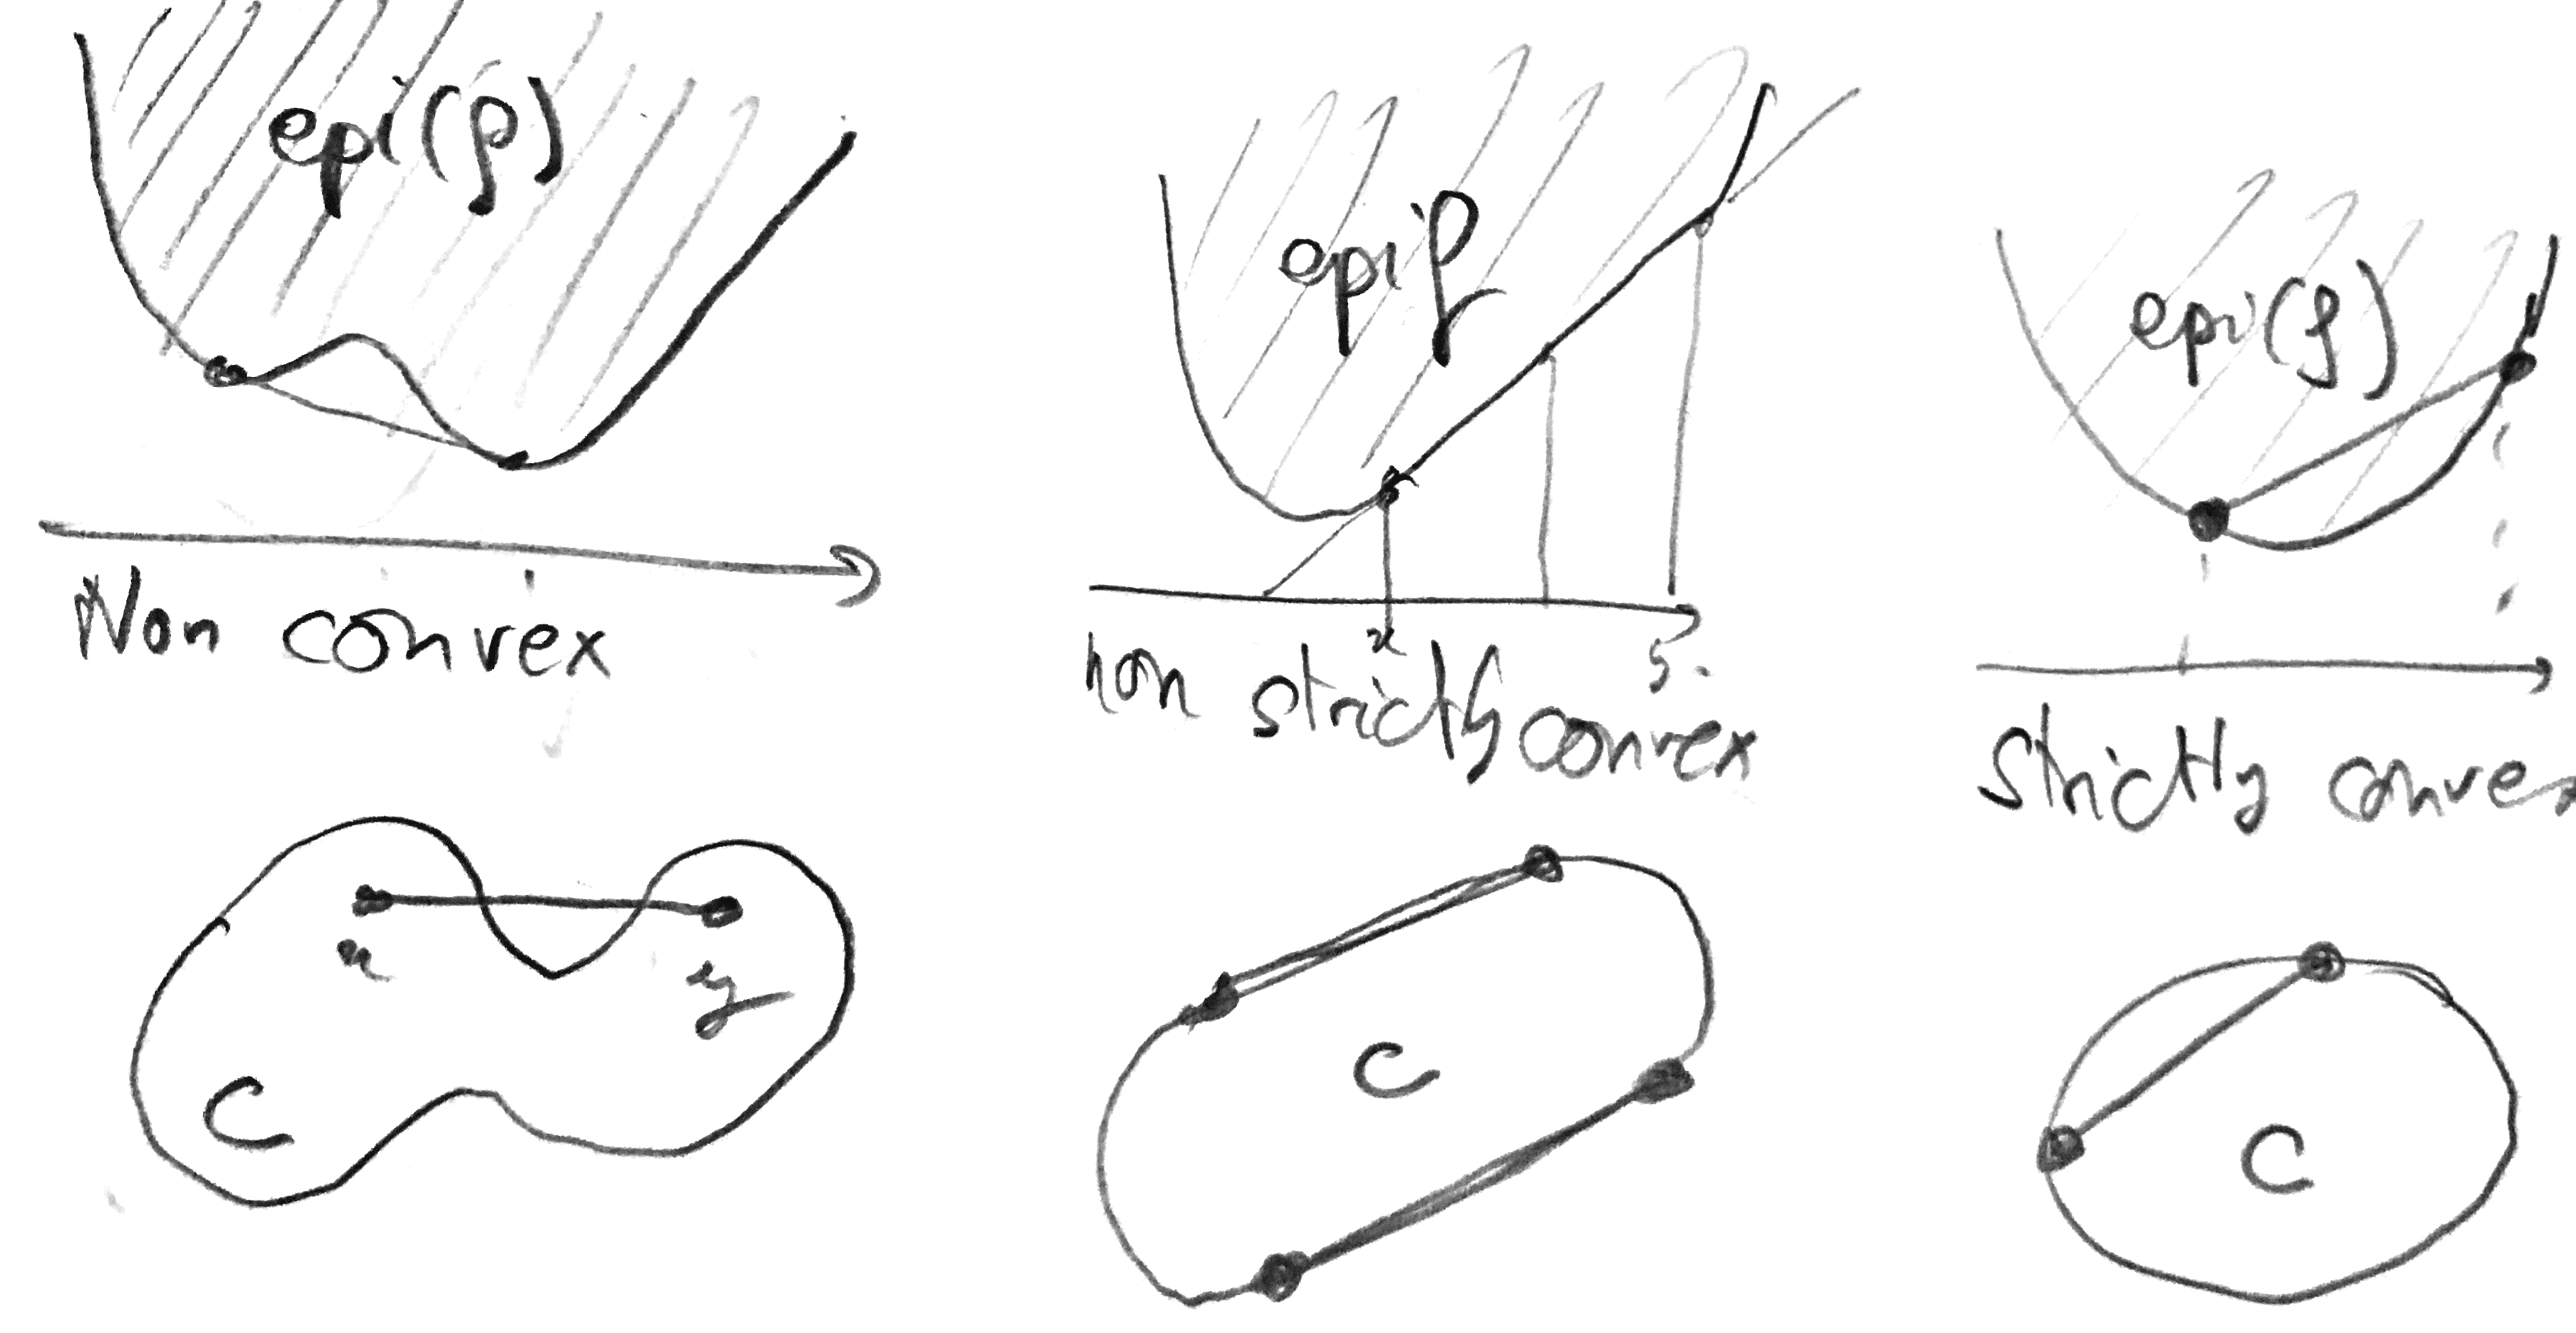
\includegraphics[width=.6\linewidth]{convexity/convex-examples}
%%
\caption{\label{fig-convex-examples}
Convexity and strict convexity for function and sets.}
\end{figure}




In the remaining part of this chapter, we consider convex function $f$ which are proper, i.e. such that $\dom(f) \neq \emptyset$, and that should be lower-semi-continuous (lsc), i.e. such that for all $x \in \Hh$, 
\eq{
	\lim\inf_{y \rightarrow x} f(y)  \geq f(x). 
}
It is equivalent to $\epi(f)$ being a closed convex set.
%
We denote $\Ga_0(\Hh)$ the set of proper convex lsc functions.

%%%%%%%%%%%%%%%%%%%%%%%%%%%%%%%%%%%%%%%%%%%%%%%%%%%%%%%%%%%%%%%%%%%%%%%%%%%%%%%%%%
\subsection{First Order Conditions}

%%%
\paragraph{Existence of minimizers.}

Before looking at first optimality conditions, one has to check that there exists minimizers, which is implied by the l.s.c. property and coercivity.

\begin{prop}
	If $f$ is l.s.c. and coercive (i.e. $f(x)\rightarrow +\infty$ as $x \rightarrow +\infty$), then there exists a minimizer $x^\star$ of $f$. 
\end{prop}

\begin{proof}
Since $f$ is coercive, it is bounded from bellow, one can consider a minimizing sequence $(x_n)_n$ such that $f(x_n) \rightarrow \min f$. 
%
Since $f$ is l.s.c., this implies that the sub-level set of $f$ are closed, and coercivity imply they are bounded, hence compact. One can thus extract from $(x_n)_n$ a converging sub-sequence $(x_{n(p)})_p$, $x_{n(p)} \rightarrow x^\star$. Lower semi-continuity implies that $\min f = \lim_p f(x_{n(p)}) \geq f(x^\star)$, and hence $x^\star$ is a minimizer.
\end{proof}

This existence proof is often called the ``direct method of calculus of variation''.
%
Note that if the function $f$ is in $\Ga_0(\Hh)$, then the set of minimizer $\argmin f$ is a closed convex set, and all local minimizers (i.e. minimizer of the function restricted to an open ball) are global one. If it is furthermore strictly convex, then there is a single minimizer. 

%%%
\paragraph{Sub-differential.}

The sub-differential at $x$ of such a $f$ is defined as
\eq{
	\partial f(x) \eqdef \enscond{u \in \Hh^*}{ \forall y, f(y) \geq f(x) + \dotp{u}{y-x} }.
}
We denote here $\Hh^* = \RR^N$ the set of ``dual'' vector. Although in finite dimensional Euclidean space, this distinction is not needed, it helps to distinguish primal from dual vectors, and recall that the duality pairing implicitly used depends on the choice of an inner product.
%
The sub-differential $\partial f(x)$ is thus the set of ``slopes'' $u$ of tangent affine planes $f(x) + \dotp{u}{z-x}$ that fits bellow the graph of $f$. 


\wrapf{convexity/subdifferential}{The subdifferential}
Note that $f$ being differentiable at $x$ is equivalent to the sub-differential being reduced to a singleton (equal to the gradient vector)
\eq{
	\partial f(x) = \{ \nabla f(x) \}. 
}
Informally, the ``size'' of $\partial f(x)$ controls how smooth $f$ is at $x$.

Note that one can have $\partial f(x) = \emptyset$, for instance if $x \notin \dom(f)$. Note also that one can still have $x \in \dom(f)$ and $\partial f(x) = \emptyset$, for instance take $f(x)=-\sqrt{1-x^2} + \iota_{[-1,1]}(x)$ at $x=\pm 1$. 

Since $\partial f(x) \subset \Hh^*$ is an intersection of half space, it is a closed convex set.
%  and it is non-empty if and only if $x \in \dom(f)$.
%
The operator $\partial f : \Hh \mapsto 2^{\Hh^*}$ is thus ``set-valued'', and we often denote this as $\partial f : \Hh \hookrightarrow \Hh^*$.

\begin{rem}[Maximally monotone operator]
The operator $\partial f$ is particular instance of so-called monotone operator, since one can check that $U=\partial f$ satisfies 
\eq{
	\foralls (u,v) \in U(x) \times U(y), \quad
		\dotp{y-x}{v-u} \geq 0. 
}
In the 1-D setting, being monotone is the same as being an increasing map.
%
Sub-differential can also be shown to be maximally monotone, in the sense that such an operator is not striclty included in the graph of another monotone operator. 
%
Note that there exists monotone maps which are not subdifferential, for instance $(x,y) \mapsto (-y,x)$. 
% 
Much of the theory of convex analysis and convex optimization can be extended to deal with arbitrary maximally monotone-maps in place of subdifferential, but we will not pursue this here.
\end{rem}

A prototypical example is the absolute value $f(x)=|\cdot|$, and writing conveniently $\partial f(x) = \partial |\cdot|(x)$, one verifies that
\eq{
	\partial |\cdot|(x) = 
	\choice{
		-1 \qifq x < 0, \\
		+1 \qifq x > 0, \\
		{[-1,1]} \qifq x=0.
	}
}

\begin{figure}
\centering
%%
\includegraphics[width=.6\linewidth]{convexity/subdiff-l1}
%%
\caption{\label{fig-subdiff-l1}
Subdifferential of the absolute value and a piecewise affine convex function.}
\end{figure}







%%%
\paragraph{First Order Conditions.}

The subdifferential is crucial for this simple but extremely important proposition.

\begin{prop}
	$x^\star$ is a minimizer of $f$ is and only if $0 \in \partial f(x^\star)$.
\end{prop}
\begin{proof}
	One has
	\eq{
		x^\star \in \argmin f
		\quad\Leftrightarrow\quad
		\pa{ \forall y, f(x^\star) \leq f(y) + \dotp{0}{x^\star-y} }
		\quad\Leftrightarrow\quad
		0 \in \partial f(x^\star).
	}
\end{proof}

%%%
\paragraph{Sub-differential calculus.}

There is a large set of calculus rules that allows to simplify the computation of sub-differentials. For decomposable function $f(x_1,\ldots,x_K)=\sum_{k=1}^K f_k(x_k)$, the sub-differential is the product of the sub-differentials
\eq{
	\partial f(x_1,\ldots,x_K) = \partial f_1(x_1) \times \ldots \times \partial f_K(x_K).
}
This can be used to compute the sub-differential of the $\ell^1$ norm $\norm{x}_1=\sum_{k=1}^N |x_k|$
\eq{
	\partial \norm{\cdot}_1(x) = \prod_{k=1}^N \partial |\cdot|(x_k)
}
which is thus an hyper rectangle. This means that, denoting $I = \supp(x)$, one has $u \in \partial \norm{\cdot}_1(x)$ is equivalent to 
\eq{
	u_I = \sign(x_I)
	\qandq
	\norm{u_{I^c}}_\infty \leq 1.
}

A tricky problem is to compute the sub-differential of the sum of two functions. If one of the two function is continuous at $x$ (i.e. it has a finite value), then 
\eq{
	\partial (f+g)(x) = \partial f(x) \oplus \partial g(x) = \enscond{u+v}{(u,v) \in \partial f(x) \times \partial g(x)}
}
where $\oplus$ thus denotes the Minkowski sum. For instance, if $f$ is differentiable at $x$, then 
\eq{
	\partial (f+g)(x) = \nabla f(x) + \partial g(x) = \enscond{\nabla f(x) + v }{ v \in \partial g(x) }.
}
Positive linear scaling is simple to handle
\eq{
	\foralls \la \in \RR_+, \quad
	\partial (\la f)(x) = \la (\partial f(x)). 
}

The chain rule for sub-differential is difficult since in general composition does not work so-well with convexity. 
%
The only simple case is composition with linear functions, which preserves convexity. Denoting $A \in \RR^{P \times N}$ and $f \in \Ga_0(\RR^P)$, one has that $f \circ A \in \Ga_0(\RR^N)$ and
\eq{
	\partial (f \circ A)(x) = A^* (\partial f)(Ax) \eqdef \enscond{A^* u}{ u \in \partial f(Ax) }. 
}


%%%
\paragraph{Normal cone.}


The sud-differential of an indicator function is a convex cone, the so-called normal cone to the constraint
\eq{
	\foralls x \in \Cc, \quad \partial \iota_\Cc(x) = \Nn_\Cc(x) \eqdef \enscond{ v }{ \foralls z \in \Cc, \dotp{z-x}{v} \leq 0 }.
}
Note that for $x \notin \Cc$, $\partial  \iota_\Cc(x) = \emptyset$.
%
For an affine space $\Cc = a+\Vv$ where $\Vv \subset \Hh$ is a linear space, then $\Nn_\Cc(x)=\Vv^\bot$ is the usual orthogonal for linear spaces. If $x \in \inter(\Cc)$ is in the interior of $\Cc$, then $\Nn_\Cc(x)=\{0\}$. In some sense, the more non-regular the boundary of $\Cc$ is at $x$, the larger is the normal cone. 






\wrapf{convexity/normal-cone}{Normal cones}
The normal cone is a way to express first order condition for constrained problem
\eq{
	\umin{x \in \Cc} f(x)
}
which reads, if $f$ is continuous
\eq{
	0 \in \partial f(x) + \partial \iota_{\Cc}(x)
	\quad\Leftrightarrow\quad
	\exists \xi \in \partial f(x), - \xi \in \Nn_\Cc(x)
	\quad\Leftrightarrow\quad
	\partial f(x) \cap (-\Nn_\Cc(x)) \neq \emptyset.
}
If $f$ is differentiable, it reads $-\nabla f(x) \in \Nn_\Cc(x)$.



%%%%%%%%%%%%%%%%%%%%%%%%%%%%%%%%%%%%%%%%%%%%%%%%%%%%%%%%%%%%%%%%%%%%%%%%%%%%%%%%%%
%%%%%%%%%%%%%%%%%%%%%%%%%%%%%%%%%%%%%%%%%%%%%%%%%%%%%%%%%%%%%%%%%%%%%%%%%%%%%%%%%%
%%%%%%%%%%%%%%%%%%%%%%%%%%%%%%%%%%%%%%%%%%%%%%%%%%%%%%%%%%%%%%%%%%%%%%%%%%%%%%%%%%
\section{Convex Duality}
\label{sec-cvx-duality}

Duality is associated to a particular formulation of the optimization problem, so that for instance making change of variables results in a different duality. 

%%%%%%%%%%%%%%%%%%%%%%%%%%%%%%%%%%%%%%%%%%%%%%%%
\subsection{Lagrange Duality}

We consider a minimization of the form
\eql{\label{eq-lagrange-primal}
	p^\star = \umin{x \in \RR^N} \enscond{ f(x) }{ Ax=y \qandq g(x) \leq 0 }
}
for a continuous convex functions $f : \Hh \rightarrow 0$, a matrix $A \in \RR^{P \times N}$ and a function $g : \Hh \rightarrow \RR^Q$ such that each of its coordinates $g_i : \Hh \rightarrow \RR$ are continuous and convex.  
%
Note that it is always the case that equality in convex program corresponds to affine ones. 
%
One can always write a convex minimization problem with positivity constraints in the form~\eqref{eq-lagrange-primal}, although there exists infinite way of doing so (each one giving a different duality formula). 

Here we have assumed for simplicity that $f$ is continuous, i.e. $\dom(f)=\RR^N$.
%
The following exposition can be generalized to $\dom(f)$ being arbitrary, but this is more technical. For the sake of simplicity, we thus assume all the constraint defining the domain are encoded in $Ax=y$ and $g(x) \leq 0$


Note that it is possible to generalized the previous Lagrange duality results by replacing ``$x \geq 0$'' by ``$X \succeq 0$'' where $X$ is a matrix (and in fact even more generally using convex cones). 

We use the following fact
\eq{
	\usup{u \in \RR^P} \dotp{r}{u} = \choice{
		0 \qifq r=0, \\
		+\infty \qifq r \neq 0, 
	}
	\qandq
	\usup{v \in \RR_+^Q} \dotp{s}{v} = \choice{
		0 \qifq s \leq 0, \\
		+\infty \text{ otherwise}, 
	}
}
to encode the constraints $r=Ax-y=0$ and $s=g(x) \leq 0$.

One can represent the constraints appearing in~\eqref{eq-lagrange-primal} conveniently using a maximization over so-called Lagrange multipliers
\eq{
	p^\star = \uinf{x} \umax{u \in \RR^P, v \in \RR_+^Q } \Ll(x,u,v) \eqdef f(x) + \dotp{Ax-y}{u} + \dotp{g(x)}{v} .
}

It is tempting to inverse the inf and the sup, and study 
\begin{align}\label{eq-lagrange-dual}
	d^\star = \usup{(u,v) \in \RR^P \times \RR_+^Q } F(u,v) &\eqdef \uinf{x}  f(x) + \dotp{Ax-y}{u} + \dotp{g(x)}{v}.
\end{align}
One remarks that $F$ is a concave function (as being the minimum of linear forms), and this ``dual'' problem is thus a maximization of a concave function. 


The following proposition is the so-called weak duality, which assert that values of the dual problems always lower bounds values of the primal one

\begin{prop}
	One always has, for all $(u,v) \in \RR^P \times \RR_+^Q$, % for $x$ such that $Ax=y, g(x) \leq 0$ and 
	\eq{
		F(u,v) \leq p^\star \qarrq d^\star \leq p^\star.
	}
\end{prop}
\begin{proof}
	Since $g(x) \leq 0 $ and $v \geq 0$, one has $\dotp{g(x)}{v} \leq 0$, and since $Ax=y$, one has $\dotp{Ax-y}{u}=0$, so that 
	\eq{
		\Ll(x,u,v) \leq f(x) \qarrq F(u,v) = \uinf{x} \Ll(x,u,v) \leq \uinf{x} f(x) = p^\star.
	}
\end{proof}

The following fundamental theorem, more difficult to prove, gives a sufficient condition (so-called qualification of the constraints) such that one actually has equality.

\begin{thm}\label{thm-strong-duality}
	If 
	\eql{\label{eq-slater} 
		\exists x_0 \in \RR^N, \quad
			Ax_0=y \qandq g(x_0)<0, 
	}
	then $p^\star=d^\star$. Furthermore, $x^\star$ and $(u^\star,v^\star)$ are  solutions of respectively~\eqref{eq-lagrange-primal} and~\eqref{eq-lagrange-dual} if and only if
	\begin{align}
		\label{eq-lagr-dual-1}  & Ax^\star=y, \quad g(x^\star) \leq 0, \quad u^\star \geq 0 \\
		\label{eq-lagr-dual-2} 0 &\in \partial f(x^\star) + A^*u^\star + \sum_i v_i^\star \partial g_i(x^\star) \\
		\label{eq-lagr-dual-3}  \foralls i, \quad & u_i^\star g_i(x^\star) = 0
	\end{align}
\end{thm}

The existence of such an $x_0$ is called ``constraint qualification'', and as written here, this corresponds to the so-called ``Slater'' qualification condition (many other weaker sufficient conditions exist). 

Condition~\eqref{eq-lagr-dual-1} is simply the primal and dual constraints. 
%
Condition~\eqref{eq-lagr-dual-2} is the first order condition for the minimization of $\Ll(x,u,v)$ over $x$.
%
Condition~\eqref{eq-lagr-dual-3} is the first order condition for the maximization of $\Ll(x,u,v)$ over $(u,v)$.
%
These three conditions are often referred to as ``Karush-Kuhn-Tucker'' (KKT) conditions, and under a constraint qualification condition, they are necessary and sufficient condition for optimality. 


The last condition $u_i^\star g_i(x^\star) = 0$ (so called ``complementary slackness'') states that if $g_i(x^\star)<0$ (the constraints is not saturated) then $u_i=0$, and also that if $u_i>0$ then $g_i(x^\star)=0$.

Note that it is possible to weaken the hypotheses of this theorem, for the linear constraints of the form $g_i(x) = \dotp{x}{h_i} - c_i \leq 0$, by replacing the $g_i(x_0)<0$ by the weaker condition $\dotp{x_0}{h_i} \leq c_i$.

One can generalize this theorem to the setting where $\dom(f)$ is not equal to $\RR^N$ (i.e. it is not continuous, and thus integrates extra constraint beside the $\leq$). In this case, one has to add the extra constraint $x_0 \in \relint(\dom(f))$.
	
Theorem~\ref{thm-strong-duality} generalizes the necessary conditions provided by Lagrange multipliers for equality constrained optimization. The setting is both more complex because one can deal with inequalities that might be saturated (so this introduce positivity constraints on the multipliers $v$) but also simpler because of convexity (which thus gives also necessary conditions).

As a simple example, we now derive the dual for a simple linear projection problem. A more complicated computation is carried over in Section~\ref{sec-duality-lasso} for the Lasso. We consider
\begin{align*}
	p^\star = \umin{Ax=y} \frac{1}{2}\norm{x-z}^2 &= \umin{x} \umax{u} \frac{1}{2}\norm{x-z}^2 + \dotp{Ax-y}{u}
	= \umax{u} F(u) = \umin{x} \frac{1}{2}\norm{x-z}^2 + \dotp{Ax-y}{u}, 
\end{align*}
where we used the fact that strong duality holds because only linear constraints are involved.
%
For each $u$, the optimal $x$ satisfies $x-z+A^*u$, i.e. $x=z-A^*u$, so that 
\eq{
	F(u) = \frac{1}{2}\norm{A^*u}^2 + \dotp{A(z-A^*u)-y}{u} = -\frac{1}{2}\norm{A^*u}^2 + \dotp{u}{Az-y}.
}
Weak duality states $p^\star \geq F(u)$ for any $u$, and $p^\star = F(u^\star)$ where the optimal $u^\star$ satisfies $AA^*u = Az-y$. If $y \in \Im(A)$, then such a $u^\star$ exists and can be chosen as $u^\star = u=(AA^*)^{-1} (Az -y)$, and the (unique) primal solution reads 
\eql{\label{eq-proj-aff}
	x^\star = \Proj_{A\cdot=y}(z) (\Id-A^+A)z - A^+y.
}

%%%%%%%%%%%%%%%%%%%%%%%%%%%%%%%%%%%%%%%%%%%%%%%%
\subsection{Legendre-Fenchel Transform}

In order to simplify and accelerate computation involving Lagrange duality, it is very convenient to introduce a particular transformation of convex functions the Legendre-Fenchel transform. In some sense, it is the canonical ``isomorphisms'' (pairing) between convex functions. In spirit, is plays a similar role for convex function as the Fourier transform for signal or images. 

For $f \in \Ga_0(\Hh)$, we define its Legendre-Fenchel transform as
\eql{\label{eq-fenchel-transf}
	f^*(u) \eqdef \usup{x} \dotp{x}{u} - f(x).
}
Being the maximum of affine functional, one obtains that $f^*$ is itself a convex function, and that in fact $f^\star \in \Ga_0(\Hh^*)$. One can prove the following fundamental bi-duality result.

\begin{thm}
One has
\eq{
	\foralls f \in \Ga_0(\Hh), \quad (f^{*})^* = f. 
}
\end{thm}

In fact, $f^*$ is convex even in the case where $f$ is not, and $f^{**}$ is the convex envelop of $f$ (i.e. the largest convex function smaller than $f$). \todo{drawing}


One has the following basic property relating the sub-differentials of $f$ and $f^*$.

\begin{prop}
One has $\partial f^* = (\partial f)^{-1}$, where the inverse of a set valued map is defined in~\eqref{eq-inv-setvalued}, and 
\eq{
	\foralls (x,y), \quad \dotp{x}{y} \leq f(x) + f^*(y)
	\qandq
	\dotp{x}{y} = f(x) + f^*(y) 
	\quad\Leftrightarrow\quad x \in \partial f^*(y)
	\quad\Leftrightarrow\quad y \in \partial f(x).
}
\end{prop}

\begin{prop}\label{prop-dual-lp}
	For $1/p+1/q=1$, 
	\eq{
		( \iota_{\norm{\cdot}_p \leq 1} )^* = \norm{\cdot}_q
		\qandq
		( \norm{\cdot}_q  )^* =  \iota_{\norm{\cdot}_p \leq 1}
	}
\end{prop}


Let us now give some example of Legendre transform. 

\begin{prop}\label{eq-example-legendre}
	For $f(x)=\frac{1}{2}\dotp{Ax}{x} - \dotp{b}{x}$ with $A$ inversible, then $f^*(u) = \frac{1}{2}\dotp{A^{-1} u}{u} - \frac{1}{2}\dotp{A^{-1} b}{b}$.
	In particular, for $f=\norm{\cdot}^2/2$, then $f^*=f$. 
	One has\todo{check}
	\eq{
		f(\cdot-z)^* = f + \dotp{z}{\cdot}, \quad
		(f + \dotp{z}{\cdot})^* = f(\cdot-z), \quad
		(\la f)^* = \la f^*(\cdot/\la).		
	}
\end{prop}
\begin{proof}
	One has $f^*(u) = \dotp{Ax^\star}{x^\star} - \dotp{b}{x^\star}$ where $x^\star$ solves
	\eq{
		u = Ax^\star-b \qarrq
		x^\star = A^{-1} u + A^{-1} b.
	}
	Hence
	\eq{
		f^*(u)  = \frac{1}{2}\dotp{A A^{-1} ( u +  b )}{A^{-1}( u +  b)} - \dotp{b}{A^{-1} (u + b)}
			= \frac{1}{2}\dotp{A^{-1} u}{u} 
			- \frac{1}{2}\dotp{A^{-1} b}{b}
	}
	
\end{proof}

%%%%
\paragraph{Legendre transform and smoothness.}

While the Fourier transform is a pairing between smoothness and decay (see Section~\ref{}), the Legendre-Fenchel is really a pairing between smoothness and strong convexity. This can be intuitively seen by the fact that the Legendre-Fenchel inverts the sub-differentials~\eqref{} and hence when the functions involved are $\Cc^2$, it inverse the Hessians 
\eq{
	\partial^2 f(x) = ( \partial^2 f^*(y) )^{-1} \quad \text{at} \quad y = \nabla f(x).
}
This relation between Hessian can be seen as implying the exchange of strong convexity and uniform bound on the Hessian, as detailed in Proposition~\ref{prop-smooth-strong}.

\begin{prop}
	One has
	\eq{
		\nabla f \text{ is $L$-Lipschitz } 
		\quad\Longleftrightarrow\quad
		\nabla f^* \text{ is $\mu$-strongly convex.} 
	}
\end{prop}

This results suggests a way to smooth any function $f$. Instead of doing a convolution, one can use the infimal convolution
\eq{
	(f \otimes g)(x) \eqdef \usup{ y+y'=x } f(y) + g(y').
}
One can check that if $(f,g)$ are convex, so is $f \otimes g$, and that the Legendre transform actually exchanges sum and inf-convolution
\eq{
	( f+g )^* = f \otimes g 
	\qandq 
	( f \otimes g )^* = f + g.
}
The Moreau-Yosida regularization of $f$ is corresponds to a $\mu$-strict-convexification of $f^*$, i.e.
\eql{\label{eq-moreau-yosida}
	f_\mu \eqdef f \otimes (\frac{1}{2\mu}\norm{\cdot}^2) = ( f^* + \frac{\mu}{2}\norm{\cdot}^2 )^*.
}
Since $f^* + \frac{\mu}{2}\norm{\cdot}^2$ is at least $\mu$-strongly convex, then $f_\mu$ as a $1/\mu$-Lipchitz gradient.

As an example, the Moreau-Yosida regularization of the absolute value reads
\eq{
	(|\cdot|_\mu)(x) = 
	\choice{
		\frac{1}{2\mu}x^2 \qifq |x| \leq \mu, \\
		|x|-\frac{\mu}{2} \qifq |x|>\mu.
	}
}
This should be compared with the regularization $\sqrt{x^2+\mu^2}$ (which is above the curve) that we used previously. \todo{add drawing}



%%%%%%%%%%%%%%%%%%%%%%%%%%%%%%%%%%%%%%%%%%%%%%%%
\subsection{Fenchel-Rockafellar Duality}

%It is possible to express the Lagrange duality in term of Fenchel transform. Indeed for instance, re-write~\eqref{eq-lagrange-primal} as
%\eq{
%	\umin{(x,z) \in \RR^N} \enscond{ f(x) }{ Ax=y, x=z \qandq g(z) \leq 0 }
%}
%and then form the Lagrange dual
%\begin{align*}
%	 \umax{u \in \RR^P, v \RR_-^Q, w \in \RR^N } &\umin{x,z}  f(x) + \dotp{Ax-y}{u} + \dotp{x-z}{w} + \dotp{g(z)}{v} \\
%	 \umax{u \in \RR^P, v \RR_-^Q, w \in \RR^N } &\umin{x} f(x) + \dotp{x}{A^*u+w} + \sum_i \umin{z} - \dotp{z}{w} + g_i(z) {v_i} \\
%\end{align*}

Very often the Lagrange dual can be expressed using the conjugate of the function $f$. We give here a particularly important example, which is often called Fenchel-Rockafellar Duality. 

We consider the following structured minimization problem
\eql{\label{eq-fench-rock-basicpb}
	p^\star = \uinf{x} f(x) + g(Ax).	
}
Re-writing it as 
\eq{
	\uinf{y=Ax} f(x) + g(y), 
}
we can form the primal-dual problem
\eq{
	\uinf{(x,y)} \usup{u} f(x) + g(y) + \dotp{Ax-y}{u}. 
}
If sufficient condition on the domain of $(f,g)$ holds (such as those stated in Theorem~\ref{}), one one can exchange the min and the max and obtains the dual problem
\begin{align}\label{eq-deriv-rock-fench}
	d^\star &= \usup{u} \umin{(x,y)} f(x) + g(y) + \dotp{Ax-y}{u} \\
	&= \usup{u} \pa{ \umin{x} \dotp{x}{A^* u} + f(x) } + \pa{ \umin{y} -\dotp{y}{u} + g(y) } 
\end{align}
which leads to the celebrated Fenchel-Rockafellar, which we summarize together with qualification sufficient condition ensuring strong duality.

\begin{thm}[Fenchel-Rockafellar]\label{thm-fenchel-Rockafellar}
If 
\eql{\label{eq-qualif-fenchrock}
	0 \in \relint( \dom(g) ) - A \relint( \dom(f) )
}
the one has the following strong duality
\begin{align}\label{eq-fenchel-Rockafellar}
	\uinf{x} f(x) + g(Ax) &= \uinf{x} \usup{u} \Ll(x,u) 
	= \usup{u} \uinf{x}\Ll(x,u)  
	= \usup{u} - f^*(-A^*u) - g^*(u)
\end{align}
\eq{
	\qwhereq  \Ll(x,u)  \eqdef f(x) + \dotp{Ax}{u}  - g^*(u).
}
Furthermore one has that $(x^\star,u^\star)$ is a pair of optimal primal-dual solutions if and only if
\eql{\label{eq-primal-dual}
	-A^* u^\star \in \partial f(x^\star)  
	\qandq
	A x^\star \in  \partial g^*(u^\star).
}
\end{thm}

Condition~\eqref{eq-qualif-fenchrock} is the constraint qualification ensuring that one can inverse the inf and the sup in~\eqref{eq-fenchel-Rockafellar}. It can be recovered from Slater's qualification condition~\eqref{eq-slater} when deriving the dual problem as in~\eqref{eq-deriv-rock-fench}.
%
The primal-dual relations~\eqref{eq-primal-dual} are the first order condition along the $x$ and the $u$ variables in minimization and maximization of $\Ll$. They are sometimes summarised in ``matrix'' form 
\eq{
	0 \in 
	\begin{pmatrix}
		\partial f & A^* \\
		-A & \partial g^*
	\end{pmatrix}
	\begin{pmatrix}
		x^\star \\
		u^\star
	\end{pmatrix}.
}
\include{chapters/optim-smooth}
%% !TEX root = ../FundationsDataScience.tex

\chapter{Non-smooth Convex Optimization}
\label{chap-conv-duality}

The main references for this chapter are~\cite{chambolle2010introduction,chambolle2016introduction,boyd2004convex}, see also~\cite{parikh2014proximal,boyd2011distributed,beck2014introduction}. 

We consider a general convex optimization problem
\eql{\label{eq-general-pbm} 
	\umin{x \in \Hh} f(x)
}
where $\Hh=\RR^p$ is a finite dimensional Hilbertian (i.e. Euclidean) space, 
and try to devise ``cheap'' algorithms with a low computational cost per iterations. The class of algorithms considered are first order, i.e. they make use of gradient information. 


%%%%%%%%%%%%%%%%%%%%%%%%%%%%%%%%%%%%%%%%%%%%%%%%%%%%%%%%%%%%%%%%%%%%%%%%%%%%%%%%%%
%%%%%%%%%%%%%%%%%%%%%%%%%%%%%%%%%%%%%%%%%%%%%%%%%%%%%%%%%%%%%%%%%%%%%%%%%%%%%%%%%%
%%%%%%%%%%%%%%%%%%%%%%%%%%%%%%%%%%%%%%%%%%%%%%%%%%%%%%%%%%%%%%%%%%%%%%%%%%%%%%%%%%
\section{Descent Methods}
\label{sec-grad-descent}

We have already encountered the gradient descent method informally in Section~\ref{} for the regularization of inverse problem. We now give a detailed analysis of the method.

%%%%%%%%%%%%%%%%%%%%%%%%%%%%%%%%%%%%%%%%%%%%%%%%%%%%%%%%%%%%%%%%%%%%%%%%%%%%%%%%%%
\subsection{Gradient Descent}

The optimization program~\eqref{eq-ip-tv-eps} is an example of unconstrained convex optimization of the form~\eqref{eq-general-pbm} where $f : \Hh \rightarrow \RR$ is a $\Cc^1$ function with Lipschitz gradient (so-called ``smooth'' function). Recall that the gradient $\nabla f : \Hh \mapsto \Hh$ of this functional (not to be confound with the discretized gradient $\nabla x \in \Hh$ of $f$) is defined by the following first order relation
\eq{
	f(x+r) = f(x) + \dotp{f}{r}_{\Hh} + O(\norm{r}_{\Hh}^2)
}
where we used $O(\norm{r}_{\Hh}^2)$ in place of $o(\norm{r}_{\Hh})$ (for differentiable function) because we assume here $f$ is of class $\Cc^1$ (i.e. the gradient is continuous). Section~\ref{eq-example-grad} shows typical examples of gradient computation.

For such a function, the gradient descent algorithm is defined as
\eql{\label{eq-grad-desc}
	\iit{x} \eqdef \it{x} - \tau_\ell \nabla f( \it{x} ), 
}
where the step size $\tau_\ell>0$ should be small enough to guarantee convergence, but large enough for this algorithm to be fast.


%%%%%%%%%%%%%%%%%%%%%%%%%%%%%%%%%%%%%%%%%%%%%%%%
\subsection{Sub-gradient Descent}

The gradient descent~\eqref{eq-grad-desc} cannot be applied on a non-smooth function $f$. One can use in place of a gradient a sub-gradient, which defines the sub-gradient descent
\eql{\label{eq-subgrad-desc}
	\iit{x} \eqdef \it{x} - \tau_\ell \it{g}
	\qwhereq
	\it{g} \in \partial f( \it{x} ).
}
The main issue with this scheme is that to ensure convergence, the iterate should go to zero. One can easily convince oneself why by looking at the iterates on a function $f(x)=|x|$.

\begin{thm}
	If $\sum_{\ell} \tau_\ell=+\infty$ and $\sum_{\ell} \tau_\ell^2 < +\infty$, then $\it{x}$ converges to a minimizer of $f$. 
\end{thm}

%%%%%%%%%%%%%%%%%%%%%%%%%%%%%%%%%%%%%%%%%%%%%%%%%%%%%%%%%%%%%%%%%%%%%%%%%%%%%%%%%%
\subsection{Projected Gradient Descent}
\label{sec-proj-grad}

We consider a generic constraint optimization problem as
\eql{\label{eq-constr}
	\umin{x \in \Cc} f(x) 
} 
where $\Cc \subset \RR^S$ is a closed convex set and $f : \RR^S \rightarrow \RR$ is a smooth convex function (at least of class $\Cc^1$). 

The gradient descent algorithm~\eqref{eq-grad-desc} is generalized to solve a constrained problem using the projected gradient descent 
\eql{\label{eq-proj-grad-desc}
	\iit{x} \eqdef \Proj_\Cc \pa{ \it{x} - \tau_\ell \nabla f( \it{x} ) }, 
}
where $\Proj_\Cc$ is the orthogonal projector on $\Cc$
\eq{
	\Proj_\Cc(x) = \uargmin{x' \in \Cc} \norm{x-x'}
}
which is always uniquely defined because $\Cc$ is closed and convex.
%
The following proposition shows that all the convergence properties of the classical gradient descent caries over to this projected algorithm.

\begin{thm}\label{thm-proj-grad}
	Theorems~\ref{thm-gradsec-strong-conv} and~\ref{thm-gradsec-non-strong-conv} still holds when replacing iterations~\eqref{eq-grad-desc} by~\eqref{eq-proj-grad-desc}.
\end{thm}

\begin{proof}
	The proof of Theorem~\ref{thm-gradsec-strong-conv} extends because the projector is contractant, 
	$\norm{\Proj_\Cc(x)-\Proj_\Cc(x')} \leq \norm{x-x'}$ so that the strict contraction properties of the gradient descent is maintained by this projection.   
\end{proof}

The main bottleneck that often prevents to use~\eqref{eq-proj-grad-desc} is that the projector is often complicated to compute. We are however lucky since for $\ell^1$ mininization, one can apply in a straightforward manner this method. 




%%%%%%%%%%%%%%%%%%%%%%%%%%%%%%%%%%%%%%%%%%%%%%%%%%%%%%%%%%%%%%%%%%%%%%%%%%%%%%%%%%
%%%%%%%%%%%%%%%%%%%%%%%%%%%%%%%%%%%%%%%%%%%%%%%%%%%%%%%%%%%%%%%%%%%%%%%%%%%%%%%%%%
%%%%%%%%%%%%%%%%%%%%%%%%%%%%%%%%%%%%%%%%%%%%%%%%%%%%%%%%%%%%%%%%%%%%%%%%%%%%%%%%%%
\section{Proximal Algorithm}

For non-smooth functions $f$, it is not possible to perform an ``explicit'' gradient descent step because the gradient is not even defined. One thus needs to replace this ``explicit''  step by an ``implicit'' one, which is possible even if $f$ is non-smooth.


%%%%%%%%%%%%%%%%%%%%%%%%%%%%%%%%%%%%%%%%%%%%%%%%
\subsection{Proximal Map }

The implicit stepping of amplitude $\tau>0$ is defined as 
\eql{\label{eq-defn-proximal}
	\foralls x, \quad
	\Prox_{\tau f}(x) \eqdef \uargmin{x'} \frac{1}{2}\norm{x-x'}^2 + f(x').
}
It amounts to minimize function $f$ locally around $x$, in a ball of radius controlled by $\tau$.
%
This the involved function $\frac{1}{2}\norm{x-\cdot}^2 + f$ is strongly convex, this operator $\Prox_{\tau f}$ is well defined and single-valued. 

When $f=\iota_\Cc$ is an indicator, the proximal map boils down to a projection $\Prox_{\iota_\Cc}=\Proj_{\Cc}$, it is thus in some sense a generalization of the projection to arbitrary function. And can also be interpreted as a projector on a level set of $f$.  An interesting feature of the proximal map is that it is a contraction, thus generalizing the well-known property of projectors.

\begin{prop}
	One has $\norm{ \prox_{f}(x)-\prox_{f}(y) } \leq \norm{x-y}$.
\end{prop}



\begin{figure}
\centering
%%
\includegraphics[width=.6\linewidth]{convexity/prox-proj}
%%
\caption{\label{fig-prox-proj}
Proximal map and projection map.}
\end{figure}


%%%
\paragraph{Examples}

The following proposition states a few simples examples.

\begin{prop}
One has
\eql{\label{eq-prox-l2-l1}
	\Prox_{\frac{\tau}{2} \norm{\cdot}^2}(x) =  \frac{x}{1+\tau}, 
	\qandq
	\Prox_{\tau \norm{\cdot}_1} = \Ss_\tau^1(x), 
}
where the soft-thresholding is defined as
\eq{
	\Ss_\tau^1(x) \eqdef ( S_\tau(x_i) )_{i=1}^p \qwhereq
	S_\tau(r) \eqdef \sign(r) (|r|-\la)_+,
}
(see also~\eqref{eq-soft-thresh}). For $A \in \RR^{P \times N}$, one has
\eql{\label{eq-prox-quad}
	\Prox_{\frac{\tau}{2}\norm{A \cdot-y}^2}(x) = (\Id_N + \tau A^* A)^{-1} ( x + \tau A^* y ).
	%= (\Id_{P} +\tau A^*A)^{-1} A^*	=  A^* (\Id_N + \tau AA^*)^{-1} 
}
\end{prop}
\begin{proof}
	The proximal map of $\norm{\cdot}_1$ was derived in Proposition~\ref{prop-equiv-sparse-thresh}.
	%
	For the quadratic case
	\eq{
		z = \Prox_{\frac{\tau}{2}\norm{A \cdot-y}^2}(x) 
		\quad\Leftrightarrow\quad 
		z-x + \tau A^*( A z - y ) = 0
		\quad\Leftrightarrow\quad
		(\Id_N + \tau A^* A) z = x + \tau A^* y.
	}
\end{proof}


Note that in some case, the proximal map of a non-convex function is well defined, for instance
$\Prox_{\tau \norm{\cdot}_0}$ is the hard thresholding associated to the threshold $\sqrt{2\tau}$, see Proposition~\ref{prop-equiv-sparse-thresh}.


%%%%%%%%%%%%%%%%%%%%%%%%%%%%%%%%%%%%%%%%%%
\subsection{Basic Properties}

We recap some useful proximal-calculus.

\begin{prop}
One has
\eq{
	\Prox_{f+\dotp{y}{\cdot}} = y + \Prox_{f}, \quad
	\Prox_{f(\cdot-y)} = y + \Prox_{f}(\cdot-y).
}
If $f(x)=\sum_{k=1}^K f(x_k)$ for $x=(x_1,\ldots,x_K)$ is separable, then
\eql{\label{eq-prox-separable}
	\Prox_{\tau f}(x) = ( \Prox_{\tau f_k}(x_k) )_{k=1}^K.
}
\end{prop}
\begin{proof}
	One has
	\eq{
		z = \Prox_{f+\dotp{y}{\cdot}}(x) 
		\quad\Leftrightarrow\quad 0 \in x-z + (\partial f(x)+y) 
		\quad\Leftrightarrow\quad 0 \in x-(z-y) + \partial f(x) 
	}
	which is the optimality condition for $z-y = \Prox_{f}(x)$.
	
	
	One has
	\eq{
		z = \Prox_{f(\cdot-y)}(x)
		\quad\Leftrightarrow\quad 0 \in x-z + \la \partial f(x-y)
		\quad\Leftrightarrow\quad 0 \in x'-(z-y) + \partial f(x') 
	}
	where we defined $x' \eqdef x-y$, and this is the optimality condition for $z-y = \Prox_{f}(x')$
\end{proof}

The following proposition is very useful.

\begin{prop}\label{prop-prox-tightframe}
	If $A \in \RR^{P \times N}$ is a tight frame, i.e. $AA^*=\Id_P$, then 
	\eq{
		\Prox_{f \circ A} = A^* \circ \Prox_{f} \circ A + \Id_N - A^* A.
	}
	In particular, if $A$ is orthogonal, then $\Prox_{f \circ A} = A^* \circ \Prox_{f} \circ A$.
\end{prop}


%%%%%%%%%%%%%%%%%%%%%%%%%%%%%%%%%%%%%%%%%%
\subsection{Related Concepts}

%%%
\paragraph{Link with sub-differential.}

For a set-valued map $U : \Hh \hookrightarrow \Gg$, we define the inverse set-valued map $U^{-1} : \Gg \hookrightarrow \Hh$ by 
\eql{\label{eq-inv-setvalued}
	h \in U^{-1}(g) 
	\quad\Longleftrightarrow\quad
	g \in U(h) 
} 
\todo{ add picture }
The following proposition shows that the proximal map is related to a regularized inverse of the sub-differential.


\begin{prop}
	One has $\Prox_{\tau f} = (\Id+\tau\partial f)^{-1}$.
\end{prop}
\begin{proof}
One has the following equivalence
\eq{
	z = \Prox_{\tau f}(x) 
	\Leftrightarrow
	0 \in z-x+\tau\partial f(z)
	\Leftrightarrow
	x \in (\Id+\tau\partial f)(z)
	\Leftrightarrow
	z = (\Id+\tau\partial f)^{-1}(x)
}	
where for the last equivalence, we have replace ``$\in$'' by ``$=$'' because the proximal map is single valued.
\end{proof}

The proximal operator is hence often referred to the ``resolvent'' $\Prox_{\tau f} = (\Id+\tau\partial f)^{-1}$ of the maximal monotone operator $\partial f$. 

%%%%
\paragraph{Link with duality.}

One has the following fundamental relation between the proximal operator of a function and of its Legendre-Fenchel transform

\begin{thm}[Moreau decomposition]
	One has
	\eq{
		\Prox_{\tau f} = \Id - \tau \Prox_{f^* / \tau}( \cdot/\tau ).
	}
\end{thm}

This theorem shows that the proximal operator of $f$ is simple to compute if and only the proximal operator of $f^*$ is also simple. 
%
As a particular instantiation, since according to , one can re-write the soft thresholding as follow
\eq{
	\Prox_{\tau \norm{\cdot}_1}(x) =  x - \tau \Proj_{\norm{\cdot}_\infty \leq 1}( x/\tau )
	 =  x -  \Proj_{\norm{\cdot}_\infty \leq \tau}( x )
	 \qwhereq
	 \Proj_{\norm{\cdot}_\infty \leq \tau}( x ) = \min(\max(x,-\tau),\tau).
}

In the special case where $f=\iota_{\Cc}$ where $\Cc$ is a closed convex cone, then
\eql{\label{eq-polar-cone}
	(\iota_{\Cc})^* = \iota_{\Cc^\circ} 
	\qwhereq
	\Cc^\circ \eqdef \enscond{y}{ \foralls x \in \Cc, \dotp{x}{y} \leq 0 } 
}	
and $\Cc^\circ$ is the so-called polar cone. Cones are fundament object in convex optimization because they are invariant by duality, in the sense of~\eqref{eq-polar-cone} (if $\Cc$ is not a cone, its Legendre transform would not be an indicator).
%
Using~\eqref{eq-polar-cone}, one obtains the celebrated Moreau polar decomposition
\eq{
	x = \Proj_{\Cc}(x) +^\bot \Proj_{\Cc^\circ}(x)
} 
where ``$+^\bot$'' denotes an orthogonal sum (the terms in the sum are mutually orthogonal). \todo{add drawing}
%
In the case where $\Cc=V$ is a linear space, this corresponds to the usual decomposition $\RR^p = V \oplus^\bot V^\bot$. 

%%%%
\paragraph{Link with Moreau-Yosida regularization.}

The following proposition shows that the proximal operator can be interpreted as performing a gradient descent step on the Moreau-Yosida smoothed version $f_\mu$ of $f$, defined in~\eqref{eq-moreau-yosida}.

\begin{prop}
	One has
	\eq{
		\Prox_{\mu f} = \Id - \mu \nabla f_\mu.
	}
\end{prop}


%%%%%%%%%%%%%%%%%%%%%%%%%%%%%%%%%%%%%%%%%%%%%%%%%%%%%%%%%%%%%%%%%%%%%%%%%%%%%%%%%%
%%%%%%%%%%%%%%%%%%%%%%%%%%%%%%%%%%%%%%%%%%%%%%%%%%%%%%%%%%%%%%%%%%%%%%%%%%%%%%%%%%
%%%%%%%%%%%%%%%%%%%%%%%%%%%%%%%%%%%%%%%%%%%%%%%%%%%%%%%%%%%%%%%%%%%%%%%%%%%%%%%%%%
\section{Primal Algorithms}

We now describe some important algorithm which assumes some structure (a so-called ``splitting'') of the minimized functional to be able to apply proximal maps on sub-functions.
%
Note that there is obviously many ways to split or structure a given initial problem, so there are many non-equivalent ways to apply a given proximal-based method to solve the problem. Finding the ``best'' way to split a problem is a bit like black magic, and there is no definite answer.
%
Also all there algorithm comes with step size and related parameters, and there is no obvious way to tune these parameters automatically (although some insight might be gained by studying convergence rate).

%%%%%%%%%%%%%%%%%%%%%%%%%%%%%%%%%%%%%%%%%%%%%%%%
\subsection{Proximal Point Algorithm}

One has the following equivalence 
\begin{align}\label{eq-proxpoint-fix}
	x^\star \in \argmin f
	&\quad\Leftrightarrow\quad
	0 \in \partial f(x^\star)
	\quad\Leftrightarrow\quad
	x^\star \in (\Id+\tau \partial f)(x^\star) \\
	&\quad\Leftrightarrow\quad
	x^\star = (\Id+\tau \partial f)^{-1}(x^\star) = \Prox_{\tau f}(x^\star).
\end{align}
This shows that being a minimizer of $f$ is equivalent to being a fixed point of $\Prox_{\tau f}$.
%
This suggest the following fixed point iterations, which are called the proximal point algorithm 
\eql{\label{eq-proximal-point}
	\iit{x} \eqdef \Prox_{\tau_\ell f}(\it{x}).
}
On contrast to the gradient descent fixed point scheme, the proximal point method is converging for any sequence of steps.

\begin{thm}
	If $0<\tau_{\min} \leq \tau_\ell \leq \ga_{\max} < +\infty$, then $\it{x} \rightarrow x^\star$ a minimizer of $f$.
\end{thm}

This implicit step~\eqref{eq-proximal-point} should be compared with a gradient descent step~\eqref{eq-grad-desc}
\eq{
	\iit{x} \eqdef (\Id+\tau_\ell \nabla f)(\it{x}).
}
One sees that the implicit resolvent $(\Id-\tau_\ell \partial f)^{-1}$ replaces the explicit step $\Id+\tau_\ell \nabla f$. For small $\tau_\ell$ and smooth $f$, they are equivalent at first order. But the implicit step is well defined even for non-smooth function, and the scheme (the proximal point) is always convergent (whereas the explicit step size should be small enough for the gradient descent to converge). This is inline with the general idea the implicit stepping (e.g. implicit Euler for integrating ODE, which is very similar to the proximal point method) is more stable. Of course, the drawback is that explicit step are very easy to implement whereas in general proximal map are hard to solve (most of the time as hard as solving the initial problem).


%%%%%%%%%%%%%%%%%%%%%%%%%%%%%%%%%%%%%%%%%%%%%%%%
\subsection{Forward-Backward}
\label{sec-fb}

It is in general impossible to compute $\Prox_{\ga f}$ so that the proximal point algorithm is not implementable.
%
In oder to derive more practical algorithms, it is important to restrict the class of considered function, by imposing some structure on the function to be minimized. We consider functions of the form
\eql{\label{eq-fb-split}
	\umin{x} \Ee(x) \eqdef f(x) + g(x)
}
where $g \in \Ga_0(\Hh)$ can be an arbitrary, but $f$ needs to be smooth.

One can modify the fixe point derivation~\eqref{eq-proxpoint-fix} to account for this special structure
\begin{align*}
 	x^\star \in \argmin f + g
	& \quad\Leftrightarrow\quad
	0 \in \nabla f(x^\star) + \partial g(x^\star) 
	\quad\Leftrightarrow\quad
	x^\star - \tau \nabla f(x^\star) \in (\Id+\tau \partial g)(x^\star) \\
	& \quad\Leftrightarrow\quad
	x^\star = ( \Id + \tau \partial g )^{-1} \circ ( \Id - \tau \nabla f ) (x^\star).
\end{align*}
This fixed point suggests the following algorithm, with the celebrated Forward-Backward
\eql{\label{eq-fb}
		\iit{x} \eqdef \Prox_{\tau_\ell g}\pa{ \it{x} - \tau_\ell \nabla f(\it{x}) }.
}


%%%
\paragraph{Derivation using surrogate functionals.}

An intuitive way to derive this algorithm, and also a way to prove its convergence, it using the concept of surrogate functional.

%
% The difficulty is the presence of the operator $A$ in the $\ldeux$ norm, which makes this problem significantly more difficult than the simple denoising by regularization\eqref{eq-regul-denoising}.

To derive an iterative algorithm, we modify the energy $\Ee(x)$ to obtain a surrogate functional $\Ee(x,\it{x})$ whose minimization corresponds to a simpler optimization problem, and define the iterations as
\eql{\label{eq-surrogate-iter}
	\iit{x} \eqdef \uargmin{x} \Ee(x,\it{x}).
}
In order to ensure convergence, this function should satisfy the following property
\eql{\label{eq-surrogate-pty}
	\Ee(x) \leq \Ee(x,x')
	\qandq
	\Ee(x,x) = \Ee(x)
}
and $\Ee(x)-\Ee(x,x')$ should be a smooth function.
%
Property \eqref{eq-surrogate-pty} guarantees that $f$ is decaying by the iterations
\eq{
	\Ee(\iit{x}) \leq \Ee(\it{x})
}
and it simple to check that actually all accumulation points of $(\it{x})_\ell$ are stationary points of $f$. 

In order to derive a valid surrogate $\Ee(x,x')$ for our functional~\eqref{eq-fb-split}, since we assume $f$ is $L$-smooth (i.e. satisfies~\eqref{eq-lipsch-grad}), let us recall the quadratic majorant~\eqref{eq-above-below-quad}
\eq{
	f(x) 
	\leq 
	f(x') + \dotp{\nabla f(x')}{x'-x} + \frac{L}{2}\norm{x-x'}^2, 
}
so that for $0 < \tau < \frac{1}{L}$, the function 
\eql{\label{eq-surrogate-ip}
	\Ee(x,x') \eqdef f(x') + \dotp{\nabla f(x')}{x'-x} + \frac{1}{2\tau}\norm{x-x'}^2 + g(x)
}
satisfies the surrogate conditions~\eqref{eq-surrogate-pty}.
%
The following proposition shows that minimizing the surrogate functional corresponds to the computation of a so-called proximal operator. 

\begin{prop}
	The update~\eqref{eq-surrogate-iter} for the surrogate~\eqref{eq-surrogate-ip} is exactly~\eqref{eq-fb}.
\end{prop}
\begin{proof}
	This follows from the fact that
	\eq{
		\dotp{\nabla f(x')}{x'-x} + \frac{1}{2\tau}\norm{x-x'}^2 
		= \frac{1}{2\tau} \norm{ x - (x'-\tau \nabla f(x'))  }^2 + \text{cst}.
	}
\end{proof}

%%%
\paragraph{Convergence of FB. }

Although we impose $\tau<1/L$ to ensure majorization property, one can actually show convergence under the same hypothesis as for the gradient descent, i.e. $0 < \tau < 2/L$, with the same convergence rates.  This means that Theorem~\ref{thm-proj-grad} for the projected gradient descent extend to FB. 

\begin{thm}\label{thm-fb-conv}
	Theorems~\ref{thm-gradsec-strong-conv} and~\ref{thm-gradsec-non-strong-conv} still holds when replacing iterations~\eqref{eq-grad-desc} by~\eqref{eq-fb}.
\end{thm}

Note furthermore that the projected gradient descent algorithm~\eqref{eq-proj-grad-desc} is recovered as a special case of~\eqref{eq-fb} when setting $J=\iota_{\Cc}$ the indicator of the constraint set, since $\Prox_{\rho J} = \Proj_{\Cc}$ in this case.

Of course the difficult point is to be able to compute in closed form $\Prox_{\tau g}$ in~\eqref{eq-fb}, and this is usually possible only for very simple function. We have already seen such an example in Section~\ref{sec-ista} for the resolution of $\ell^1$-regularized inverse problems (the Lasso).


%%%%%%%%%%%%%%%%%%%%%%%%%%%%%%%%%%%%%%%%%%%%%%%%
\subsection{Douglas-Rachford}

We consider here the structured minimization problem
\eql{\label{eq-struct-dr}
	\umin{x \in \RR^p} f(x) + g(x), 
}
but on contrary to the Forward-Backward setting studied in Section~\ref{sec-fb}, no smoothness is imposed on $f$. We here suppose that we can compute easily the proximal map of $f$ and $g$.

\begin{exmp}[Constrained Lasso]
An example of a problem of the form~\eqref{eq-struct-dr} where one can apply Douglas-Rachford is the noiseless constrained Lasso problem~\eqref{eq-lasso-constr-ip}
\eq{
	\umin{Ax=y} \norm{x}_1
}
where one can use $f=\iota_{\Cc_y}$ where $\Cc_y \eqdef \enscond{x}{Ax=y}$ and $g=\norm{\cdot}_1$.
%
As noted in Section~\ref{eq-linearprog-lasso}, this problem is equivalent to a linear program.
%
The proximal operator of $g$ is the soft thresholding as stated in~\eqref{eq-prox-l2-l1}, while the proximal operator of $g$ is the orthogonal projector on the affine space $\Cc_y$, which can be computed by solving a linear system as stated in~\eqref{eq-proj-aff} (this is especially convenient for inpainting problems or deconvolution problem where this is achieved efficiently).
\end{exmp}

The Douglas-Rachford iterations read
\eql{\label{eq-dr-iter} 
	 \iit{\tilde x} \eqdef \pa{1-\frac{\mu}{2}} \it{\tilde x} + 
	\frac{\mu}{2} \rProx_{\tau g}( \rProx_{\tau f}( \it{\tilde x} )  ) 
	\qandq \iit{x} \eqdef \Prox_{\tau f}( \iit{\tilde x}), 
}
where we have used the following shortcuts
\eq{   	
	\rProx_{\tau f}(x) = 2\Prox_{\tau f}(x)-x .
}
One can show that for any value of $\tau>0$, any $0 < \mu < 2$,  and any $\tilde x_0$, $\it{x} \rightarrow x^\star$ which is a minimizer of $f+g$.

Note that it is of course possible to inter-change the roles of $f$ and $g$, which defines another set of iterations.

%%%
\paragraph{More than two functions.}

Another sets of iterations can be obtained by ``symetrizing'' the algorithm. More generally, if we have $K$ functions $(f_k)_k$, we re-write 
\eq{
	\umin{x} \sum_k f_k(x) = \umin{X=(x_1,\ldots,x_k)} f(X)+g(X)
	\qwhereq
	f(X) = \sum_k f_k(x_k)
	\qandq
	g(X)=\iota_{\Delta}(X)
}
where $\Delta=\enscond{X}{x_1=\ldots=x_k}$ is the diagonal. The proximal operator of $f$ is 
\eq{
	\Prox_{\tau f}(X)=\Proj_\De(X)=(\bar x,\ldots,\bar x) 
	\qwhereq
	\bar x = \frac{1}{K}\sum_k x_k
}
while the proximal operator of $f$ is easily computed from those of the $(f_k)_k$ using~\eqref{eq-prox-separable}. One can thus apply DR iterations~\eqref{eq-dr-iter}.

%%%
\paragraph{Handling a linear operator.}

One can handle a minimization of the form~\eqref{eq-splitting-primal-dual} by introducing extra variables
\eq{
	\uinf{x} f_1(x) + f_2(Ax) = \uinf{z=(x,y)} f(z)+g(z)
	\qwhereq
	\choice{
		f(z)=f_1(x)+f_2(y) \\
		g(z)=\iota_\Cc(x,y),
	}
}
where $\Cc=\enscond{(x,y)}{Ax=y}$. This problem can be handled using DR iterations~\eqref{eq-dr-iter}, since the proximal operator of $f$ is obtained from those of $(f_1,f_2)$ using~\eqref{eq-prox-separable}, while the proximal operator of $g$ is the projector on $\Cc$, which can be computed in two alternative ways as the following proposition shows.

\begin{prop}One has
\eql{\label{eq-proj-axy}
	\Proj_{\Cc}(x,y) = (x+A^*\tilde y,y-\tilde y) = (\tilde x,A\tilde x)
	\qwhereq
	\choice{
		\tilde y \eqdef (\Id_P+AA^*)^{-1}(Ax-y) \\
		\tilde x \eqdef (\Id_N+A^*A)^{-1}(A^*y+x).
	}
}
\end{prop}
\begin{proof}\todo{todo}
\end{proof}

\begin{rem}[Inversion of linear operator]\label{rem-inv-lin}
	At many places (typically to compute some sort of projector) one has to invert matrices of the form 
	$AA^*$, $A^*A$, $\Id_P+AA^*$ or $\Id_N+A^*A$ (see for instance~\eqref{eq-proj-axy}).
	There are some case where this can be done efficiently.
	Typical examples where this is simple are inpainting inverse problem where $AA^*$ is diagonal, and deconvolution or partial Fourier measurement (e.g. fMRI) for which $A^*A$ is diagonalized using the FFT.
	%
	If this inversion is too costly, one needs to use more advanced methods, based on duality, which allows to avoid trading the inverse $A$ by the application of $A^*$. They are however typically converging more slowly.
\end{rem}

%%%%%%%%%%%%%%%%%%%%%%%%%%%%%%%%%%%%%%%%%%%%%%%%%%%%%%%%%%%%%%%%%%%%%%%%%%%%%%%%%%
%%%%%%%%%%%%%%%%%%%%%%%%%%%%%%%%%%%%%%%%%%%%%%%%%%%%%%%%%%%%%%%%%%%%%%%%%%%%%%%%%%
%%%%%%%%%%%%%%%%%%%%%%%%%%%%%%%%%%%%%%%%%%%%%%%%%%%%%%%%%%%%%%%%%%%%%%%%%%%%%%%%%%
\section{Dual and Primal-Dual Algorithms}

Convex duality, detailed in Section~\ref{sec-cvx-duality} (either from the Lagrange or the Fenchel-Rockafellar point of view -- which are essentially equivalent), is very fruitful to derive new optimization algorithm or to apply existing algorithm on a dual reformulation.

%%%%%%%%%%%%%%%%%%%%%%%%%%%%%%%%%%%%%%%%%%%%%%%%
\subsection{Forward-backward on the Dual}
\label{sec-fb-dual}

Let us illustrate first the idea of applying a known algorithm to the dual problem. We consider here the structured minimization problem associated to Fenchel-Rockafellar duality~\eqref{eq-fench-rock-basicpb}
\eql{\label{eq-splitting-primal-dual}
	p^\star = \uinf{x} f(x) + g(A x), 
}
but furthermore assume that $f$ is $\mu$-strongly convex, and we assume for simplicity that both $(f,g)$ are continuous. If $f$ were also smooth (but it needs to be!), one could think about using the Forward-Backward algorithm~\eqref{eq-fb}. But the main issue is that in general $\Prox_{\tau g \circ A}$ cannot be computed easily even if one can compute $\Prox_{\tau g \circ A}$. An exception to this is when $A$ is a tight frame, as exposed in Proposition~\ref{prop-prox-tightframe}, but in practice it is rarely the case. 

\begin{exmp}[TV denoising]
A typical example, which was the one used by Antonin Chambolle~\cite{chambolle-algo-tv} to develop this class of method, is the total varation denoising
\eq{
	\umin{x} \frac{1}{2}\norm{y-x}^2 + \la \norm{\nabla x}_{1,2}
}
where $\nabla x \in \RR^{N \times d}$ is the gradient (a vector field) of a signal ($d=1) $or image ($d=2$) $x$, and $\norm{\cdot}_{1,2}$ is the vectorial-$\ell^1$ norm (also called $\ell^1-\ell^2$ norm), such that for a $d$-dimensional vector field $(v_i)_{i=1}^p$ 
\eq{
	\norm{v}_{1,2} \eqdef \sum_i \norm{v_i}.
}	
Here 
\eq{
	f=\frac{1}{2}\norm{\cdot-y}^2
	\qandq
	g=\la\norm{\cdot}_{1,2}
}
so that $f$ is $\mu=1$ strongly convex, and one sets $A=\nabla$ the linear operator.
\end{exmp}


Applying Fenchel-Rockafellar Theorem~\ref{thm-fenchel-Rockafellar} (since strong duality holds, all involved functions being continuous), one has that 
\eq{
	p^\star = \usup{u}  - g^*(u) - f^*(-A^*u).
}
But more importantly, since $f$ is $\mu$-strongly convex, one has that $f^*$ is smooth with a $1/\mu$-Lipschitz gradient. One can thus use the Forward-Backward algorithm~\eqref{eq-fb} on (minus the energy of) this problem, which reads
\eq{
	\iit{u} = \Prox_{\tau_k g^*}\pa{ \it{u} + \tau_k A \nabla f^*( A^* \it{u} ) }.
}
To guarantee convergence, the step size $\tau_k$ should be smaller than $2/L$ where $L$ is the Lipschitz constant of $A \circ \nabla f^* \circ A^*$, which is smaller than $\norm{A}^2/\mu$. 

Last but not least, one some (not necessarily unique) dual minimizer $u^\star$ is computed, the primal-dual relationships~\eqref{eq-primal-dual} ensures that one retrieves the unique primal minimizer $x^\star$ as
\eq{
	-A^* u^\star \in \partial f(x^\star)  
	\quad\Leftrightarrow\quad
	x^\star \in (\partial f)^{-1}( -A^* u^\star ) = \partial f^*( -A^* u^\star )
	\quad\Leftrightarrow\quad
	 x^\star = \nabla f^*( -A^* u^\star )
}
where we used here the crucial fact that $f^*$ is smooth.

\begin{exmp}[TV denoising]
In the particular case of the TV denoising problem, one has
\eq{
	g^* = \iota_{\norm{\cdot}_{\infty,2} \leq \la}
	\qwhereq
	\norm{v}_{\infty,2} \eqdef \umax{i} \norm{v_i}
	\qarrq
	\Prox_{\tau g^*}(u) = \pa{ \min( \norm{v_i},\la ) \frac{v_i}{\norm{v_i}} }
}
\eq{
	f^\star(h) = \frac{1}{2}\norm{h}^2+\dotp{h}{y}
	\qandq
	\nabla f^\star(h) = h + y.
}
Furthermore, $\mu=1$ and $A^*A=\Delta$ is the usual finite difference approximation of the Laplacian, so that $\norm{A}^2=\norm{\Delta}=4d$ where $d$ is the dimension.
\end{exmp}


%%%%%%%%%%%%%%%%%%%%%%%%%%%%%%%%%%%%%%%%%%%%%%%%
\subsection{Primal-Dual Splitting}

We now comeback to the more general structure problem of the form~\eqref{eq-splitting-primal-dual}, which we consider in primal-dual form as
\begin{align}\label{eq-splitting-primal-dual-bis}
	\uinf{x} f(x) + g(Ax) 
	= \usup{u} \uinf{x} f(x) + \dotp{Ax}{u}  - g^*(u), 
\end{align}
but we do not suppose anymore that $f$ is strongly convex. 

A typical instance of such a problem is for the TV regularization of the inverse problem $\Kk x=y$, which corresponds to solving
\eq{
	\umin{x} \frac{1}{2}\norm{y-\Kk x}^2 + \la \norm{\nabla x}_{1,2}.
}
where $A=\nabla$, $f(x)=\frac{1}{2}\norm{y-\Kk \cdot}^2$ and $g=\la \norm{\cdot}_{1,2}$.
%
Note however that with such a splitting, one will have to compute the proximal operator of $f$, which, following~\eqref{eq-prox-quad}, requires inverting either $\Id_P+AA^*$ or $\Id_N+A^*A$, see Remark~\ref{rem-inv-lin}. 

A standard primal-dual algorithm, which is detailed in~\cite{}, reads
\begin{align*}
	\iit{z} &\eqdef \Prox_{\sigma g^*}( \it{z} + \sigma A( \it{\tilde x}) \\
	\iit{x} &\eqdef \Prox_{\tau f}(  \it{x}-\tau A^*(\iit{z}) ) \\
	 \it{\tilde x} &\eqdef \iit{x} + \theta (\iit{x} - \it{x}) 
\end{align*}
if $0 \leq \th \leq 1$ and $\sigma \tau \norm{K}^2<1$, then $\it{x}$ converges to a minimizer of~\eqref{eq-splitting-primal-dual-bis} .

%\include{chapters/sparse-theory}
%\include{chapters/compressed-sensing}
%%!TEX root = ../FundationsDataScience.tex

\chapter{Machine Learning}


% Refs \cite{rosasco2017notes,friedman2001elements,murphy2012machine}

This chapter gives a rapid overview of the main concepts in machine learning. The goal is not to be exhaustive, but to highlight representative problems and insist on the distinction between unsupervised (vizualization and clustering) and supervised (regression and classification) setups. We also shed light on the tight connexions between machine learning and inverse problems.

While imaging science problems are generally concern with processing a single data (e.g. an image), machine learning problem is rather concern with analysing large collection of data. The focus (goal and performance measures) is thus radically different, but quite surprisingly, it uses very similar tools and algorithm (in particular linear models and convex optimization). 


%%%%%%%%%%%%%%%%%%%%%%%%%%%%%%%%%%%%%%%%%%%%%%%%%%
%%%%%%%%%%%%%%%%%%%%%%%%%%%%%%%%%%%%%%%%%%%%%%%%%%
%%%%%%%%%%%%%%%%%%%%%%%%%%%%%%%%%%%%%%%%%%%%%%%%%%
\section{Unsupervised Learning}

In unsupervised learning setups, one observes $n$ points $(x_i)_{i=1}^n$. 
%
The problem is now to infer some properties for this points, typically for vizualization or unsupervised classication (often called clustering). 
%
For simplicity, we assume the data are points in Euclidean space $x_i \in \RR^p$ ($p$ is the so-called number of features). These points are conveniently stored as the rows of a matrix $X \in \RR^{n \times d}$.


%%%%%%%%%%%%%%%%%%%%%%%%%%%%%%%%%%%%%%%%%%%%%%%%%%
\subsection{Dimensionality Reduction and PCA}

Dimensionality reduction is useful for vizualization. It can also be understood as the problem of feature extraction (determining which are the relevant parameters) and this can be later used for doing other tasks more efficiently (faster and/or with better performances). 
%
The simplest method is the Principal Component Analysis (PCA),  which performs an orthogonal linear projection on the principal axes (eigenvectors) of the covariance matrix.

%%%
\paragraph{Presentation of the method.}

The empirical mean is defined as 
\eq{
    \hat m \eqdef \frac{1}{n} \sum_{i=1}^n x_i \in \RR^p
} 
and  covariance
\eql{\label{eq-emp-cov}
 	\hat C \eqdef \frac{1}{n} \sum_{i=1}^n (x_i-\hat m) (x_i-\hat m)^* \in \RR^{p \times p}. 
}
Denoting $\tilde X \eqdef X - 1_p \hat m^*$, one has $\hat C=\tilde X^*
\tilde X/n$. 

Note that if the points $(x_i)_i$ are modelled as i.i.d. variables, and denoting $\xp$ one of these random variables, one has, using the law of large numbers, the almost sure convergence as $n \rightarrow +\infty$
\eql{\label{eq-cov-approx}
	\hat m \rightarrow m \eqdef \EE(\xp)
	\qandq
	\hat C \rightarrow C \eqdef \EE((\xp-m)(\xp-m)^*).
}
Denoting $\mu$ the distribution (Radon measure) on $\RR^p$ of $\xp$, one can alternatively write
\eq{
	m = \int_{\RR^p} x \d\mu(x)
	\qandq
	C = \int_{\RR^p} (x-m)(x-m)^* \d\mu(x).	
}


\begin{figure}
\centering
\begin{tabular}{@{}c@{}c@{}}
\includegraphics[width=.25\linewidth]{ml/pca-nn/cov}&
\includegraphics[width=.4\linewidth]{ml/pca-nn/svd}\\
$C$ & SVD of $C$
\end{tabular}
\caption{\label{fig-cov}
Empirical covariance of the data and its associated singular values. 
}
\end{figure}


\wrapf{ml/variance}{PCA main axes capture variance}
The PCA ortho-basis, already introduced in Section~\ref{prop-svd}, corresponds to the right singular vectors of the centred data matrix, as defined using the (reduced) SVD decomposition
\eq{
 	\tilde X = \sqrt{n} U \diag(\si) V^*
}
where $U \in \RR^{n \times r}$ and $V \in \RR^{p \times r}$, and where $r=\rank(\tilde X) \leq \min(n,p)$. 
%
We denote $V=(v_k)_{k=1}^r$ the orthogonal columns (which forms an orthogonal system of eigenvectors of $\hat C = V \diag(\si^2) V^\top$), $v_k \in \RR^p$. The intuition is that they are the main axes of ``gravity'' of the point cloud  $(x_i)_i$ in $\RR^p$.
%
We assume the singular values are ordered, $\si_1 \geq \ldots \geq \si_r$, so that the first singular values capture most of the variance of the data. 

Figure~\ref{fig-cov} displays an example of covariance and its associated spectrum $\si$. The points $(x_i)_i$ correspond to the celebrated
IRIS dataset\footnote{\url{https://en.wikipedia.org/wiki/Iris_flower_data_set}} of Fisher. This dataset consists of 50 samples from each of three species of Iris (Iris setosa, Iris virginica and Iris versicolor). The dimensionality of the features is $p=4$, and the dimensions corresponds to the length and the width of the sepals and petals. 

The PCA dimensionality reduction embedding $x_i \in \RR^p \mapsto z_i \in \RR^d$ in dimension $d \leq p$ is obtained by projecting the data on the first $d$ singular vector
\eql{\label{eq-pca-1}
	z_i \eqdef ( \dotp{x_i-m}{v_k} )_{k=1}^d \in \RR^d. 
}
From these low-dimensional embedding, one can reconstruct back an approximation as
\eql{\label{eq-pca-2}
	\tilde x_i \eqdef m+\sum_k z_{i,k} v_k \in \RR^p.
}
One has that $\tilde x_i = \Proj_{\tilde T}(x_i)$ where $\tilde T \eqdef m + \Span_{k=1}^d(v_k)$ is an affine space.

Figure~\ref{fig-pca} shows an example of PCA for 2-D and 3-D vizualization.

\begin{figure}
\centering
\begin{tabular}{@{}c@{\hspace{5mm}}c@{}}
\includegraphics[width=.4\linewidth]{ml/pca-nn/points-2d}&
\includegraphics[width=.4\linewidth]{ml/pca-nn/points-3d}
\end{tabular}
\caption{\label{fig-pca}
2-D and 3-D PCA vizualization of the input clouds. 
}
\end{figure}


%%%
\paragraph{Optimality analysis.}

\wrapfSimple{ml/pca-maths/pca-maths-1}
We now show that among all possible linear dimensionality reduction method, PCA is optimal in sense of $\ell^2$ error. 
%
To simplify, without loss of generality (since it can be subtracted from the data) we assume that empirical mean is zero $\hat m=0$ so that $X=\tilde X$. 

We recall that $X=\sqrt{n} U \diag(\si) V^\top$ and $\hat C = \frac{1}{n} X^\top X = U \La U^\top$ where $\La = \diag(\la_i=\si_i^2)$, where $\la_1 \geq \ldots \geq \la_r$.  

\wrapfSimple{ml/pca-maths/pca-maths-2}
The following proposition shows that PCA is optimal in term of $\ell^2$ distance if one consider only affine spaces. This means that we consider the following compression/decompression to a dimension $k$ (i.e. dimensionality reduction and then expansion) 
\eql{\label{eq-pca-nonconvex}
	\umin{R,S} \enscond{
		f(R,S) \eqdef \sum_i \norm{x_i-R S^\top x_i}_{\RR^p}^2
		}{ R,S \in \RR^{p \times k} }
}
Note that this minimization is a priori not trivial to solve because, although $f(\cdot,S)$ and $f(R,\cdot)$ are convex, $f$ is not jointly convex. So iteratively minimizing on $R$ and $S$ might fail to converge to a global minimizer.
%
This section aims at proving the following theorem.

\begin{thm}\label{thm-pca-optim}
	A solution of~\eqref{eq-pca-nonconvex} is $S=R=V_{1:k} \eqdef [v_1,\ldots,v_k]$.
\end{thm}

Note that using such a compressor $R$ and decompressor $R=S$ corresponds exactly to the PCA method~\eqref{eq-pca-1} and~\eqref{eq-pca-2}.

We first prove that one can restrain its attention to orthogonal projection matrix.

\begin{lem}
	One can assume $S=R$ and $S^\top S = \Id_{k\times k}$.
\end{lem}
\begin{proof}
	We consider an arbitrary pair $(R,S)$. Since the matrix $R S^\top$ has rank $k' \leq k$, let $W \in \RR^{p \times k'}$ be an ortho-basis of $\Im(RS^\top)$, so that $W^\top W = \Id_{k' \times k'}$. We remark that 
	\eq{
		\uargmin{z} \norm{x-Wz}^2 = W^\top x
	}
	because the first order condition for this problem reads $W^\top(Wz-x)=0$.
	%	
	Hence, denoting $RS^\top x_i = Wz_i$ for some $z_i \in \RR^{k'}$
	\eq{
		f(R,S) = \sum_i \norm{x_i - RS^\top x_i}^2 = \sum_i \norm{x_i - W z_i}^2 \geq \sum_i \norm{x_i - W W^\top x_i}^2
		\geq  f(\tilde W,\tilde W).
	}
	were we have extended $W$ in an orthogonal matrix $\tilde W \in \RR^{p \times k}$ where $\tilde W_{1:k'}=W$.
\end{proof}

\begin{lem}
	Denoting $C \eqdef XX^\top \in \RR^{p \times p}$, an optimal $S$ is obtained by solving
	\eq{
		\umax{S \in \RR^{p \times k}} \enscond{\tr(S^\top C S^\top)}{ S^\top S=\Id_{k} }.
	}
\end{lem}
\begin{proof}
	Using the previous lemma, one can consider only $R=S$ with $S^\top S=\Id_{k}$ so that one needs to solve
	\eq{
		f(S,S) = \sum_i \norm{x_i SS^\top x_i}^2
		= \sum_i \norm{x_i}^2 - 2 x_i^\top S S^\top x_i + x_i^\top S(S^\top S) S^\top x_i.
	}
	Using that $S^\top S=\Id_k$, one has
	\eq{
		f(S,S) = \text{cst} - \sum_i x_i^\top S S^\top x_i
		= - \sum_i \tr(x_i^\top S S^\top x_i)
		= - \sum_i \tr(S^\top x_i x_i^\top S )
		= - \tr( S^\top (\sum_i x_i x_i^\top) S ).
	}
\end{proof}

The next lemma provides an upper bound on the quantity being minimized as the solution of a convex optimization problem (a linear program). The proof of the theorem follows by showing that this upper bound is actually reached, which provides a certificate of optimality.  

\begin{lem}\label{lem-upper-bound-pca}
	Denoting $C=V \La V^\top$, one has 
	\eql{\label{eq-variational-pca}
		\tr(S^\top C S) \leq \umax{\be \in \RR^p}
			\enscond{ \sum_{i=1}^p \la_i \be_i }{ 0 \leq \be \leq 1, \sum_i \be_i \leq k }
			= \sum_{i=1}^k \la_i
	}
	i.e. the maximum on the right hand size is $\be=(1,\ldots,1,0,\ldots,0)$.
\end{lem}
\begin{proof}
	We extend $V \in \RR^{p \times k}$ into an orthogonal matrix $\tilde V \in \RR^{p \times p}$ (i.e. $\tilde V_{1:r}=V$) such 
	that $\tilde V\tilde V^\top = \tilde V^\top V = \Id_p$. Similarly we extend $\La$ into $\tilde\La$ by adding zeros, so that $C=\tilde V \tilde \La \tilde V^\top$.  One has
	\eq{
		\tr(S^\top C S) = \tr(S^\top \tilde V \tilde \La \tilde V^\top S)
		= \tr(B^\top \La B) = \tr(\La BB^\top) = \sum_{i=1}^p \la_i \norm{b_i}^2
		= \sum_i \la_i \be_i
	}
	where we denoted $B \eqdef V^\top S \in \RR^{p \times k}$, $(b_i)_{i=1}^p$ with $b_i \in \RR^k$ are the rows of $B$ and $\be_i \eqdef \norm{b_i}^2 \geq 0$.
	%
	One has
	\eq{
		B^\top B = S^\top \tilde V \tilde V^\top S = S^\top S = \Id_k, 
	}
	so that the columns of $B$ are orthogonal, and thus
	\eq{
		\sum_i \be_i = \sum_i \norm{b_i}^2 = \norm{B}_{\text{Fro}}^2 = \tr(B^\top B) = \tr(B^\top B) = k.
	}		
	
	\begin{figure}
\centering
\begin{tabular}{@{}c@{\hspace{10mm}}c@{\hspace{10mm}}c@{}}
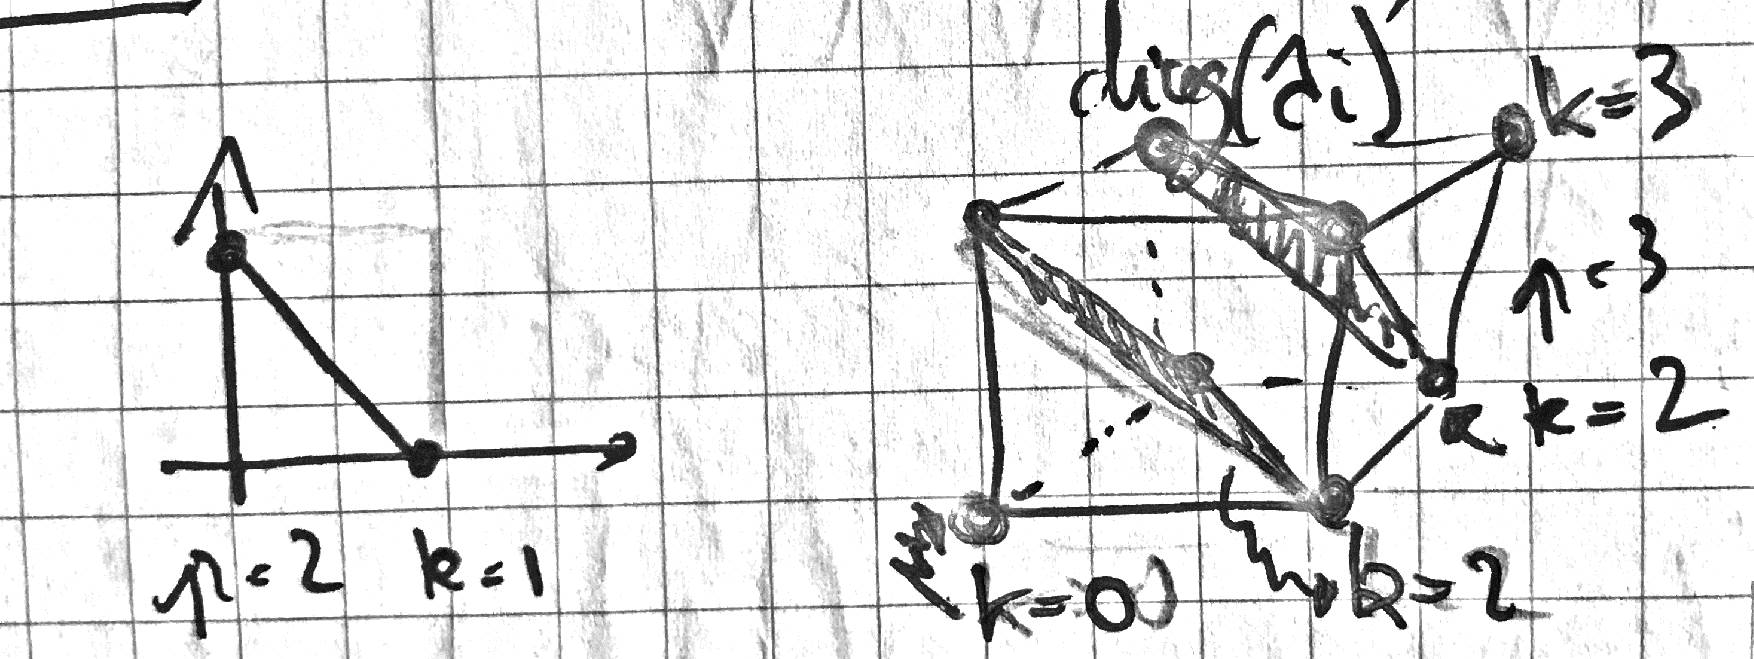
\includegraphics[width=.3\linewidth]{ml/pca-maths/pca-maths-3}&
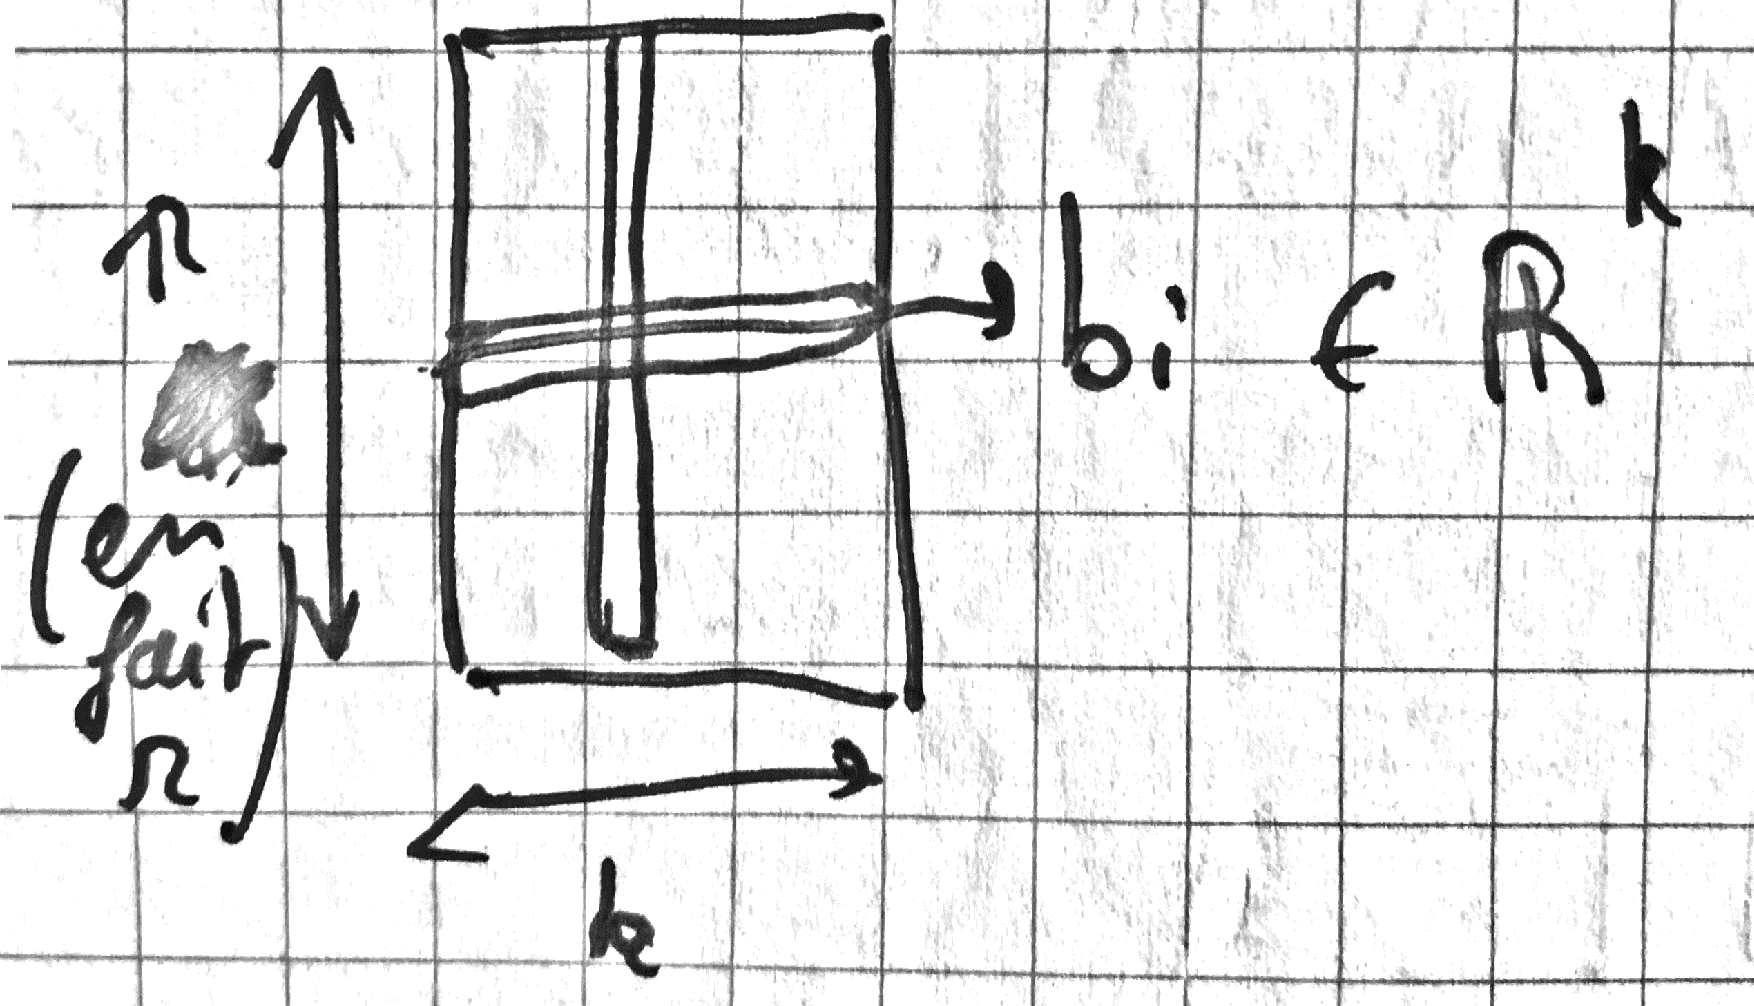
\includegraphics[width=.2\linewidth]{ml/pca-maths/pca-maths-4}&
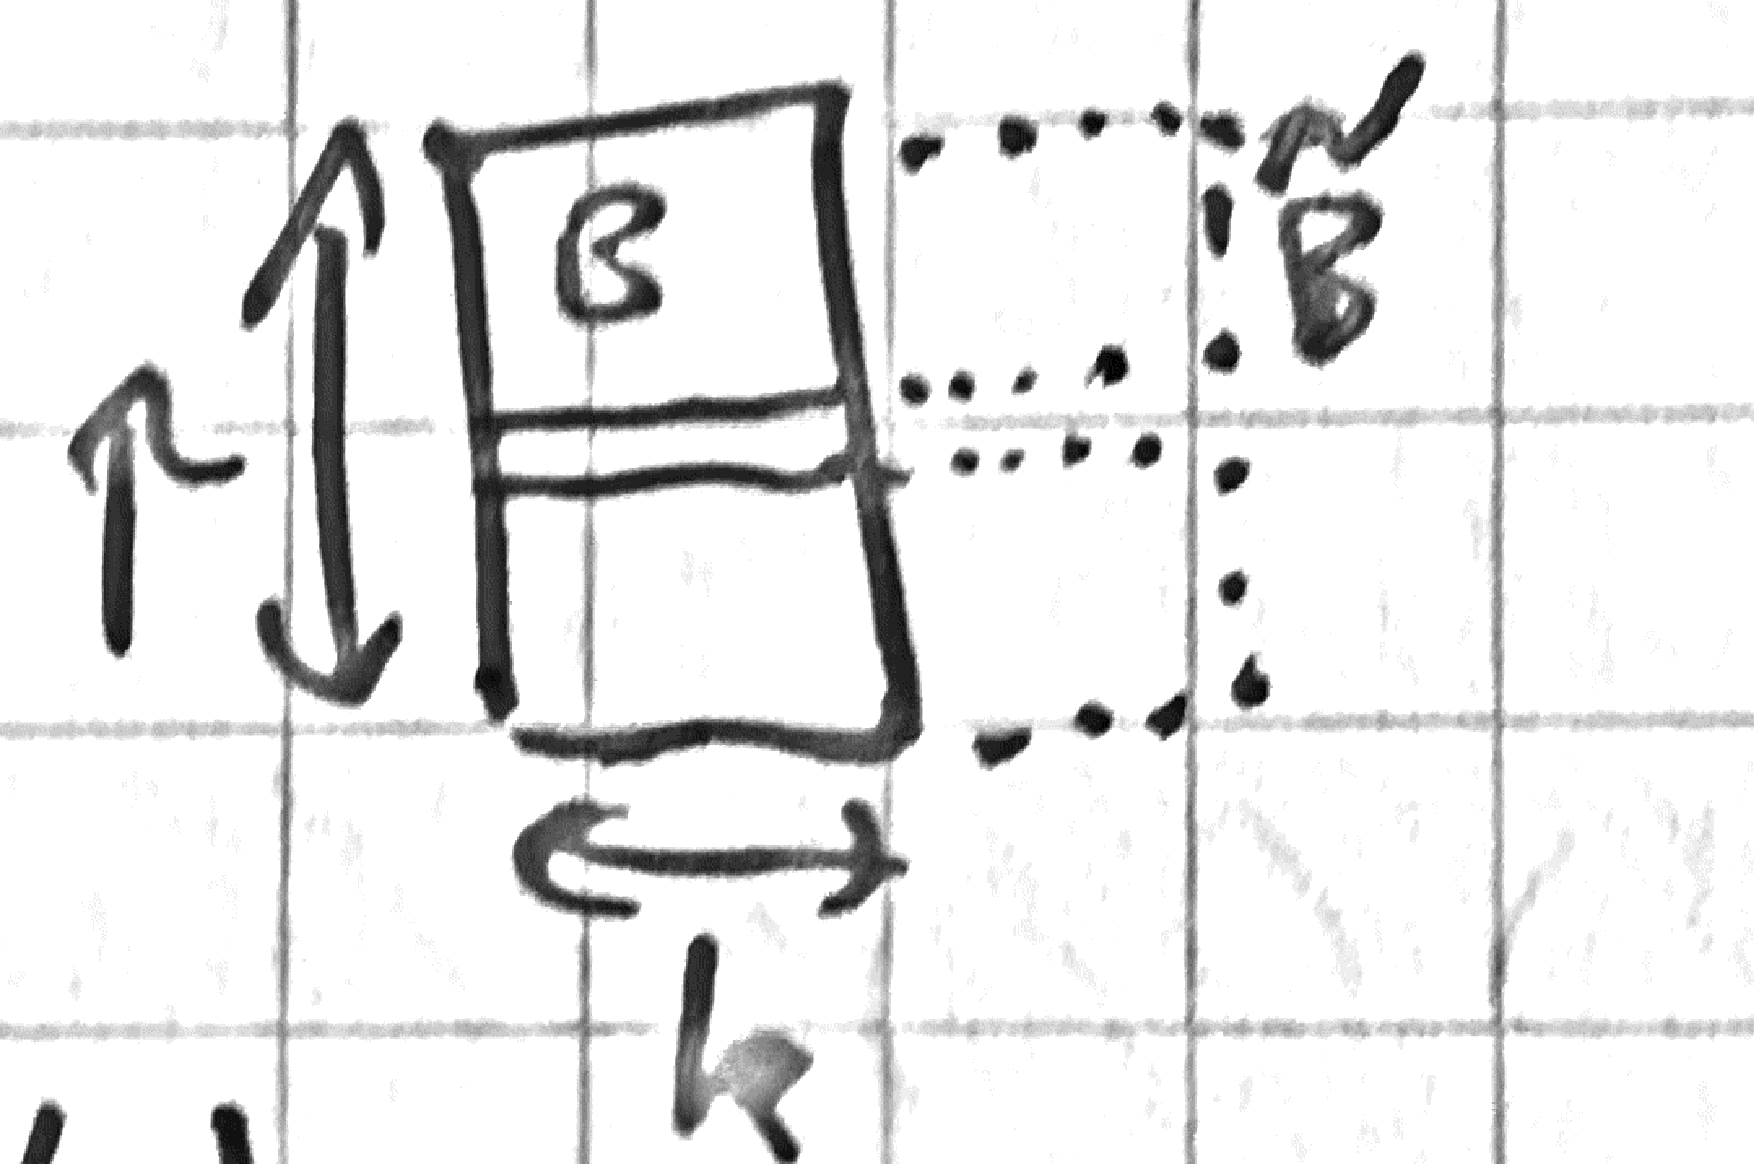
\includegraphics[width=.2\linewidth]{ml/pca-maths/pca-maths-5}
\end{tabular}
\caption{\label{fig-pca-var-proof}
Left: proof of the rightmost inequality in~\eqref{eq-variational-pca}. Middle: matrix $B$, right: matrix $\tilde B$. 
}
\end{figure}


	We extend the $k$ columns of $b$ into an orthogonal basis $\tilde B \in \RR^{p \times p}$ such that $\tilde B \tilde B^\top = \tilde B^\top \tilde = \Id_p$, so that 
	\eq{
		0 \leq \be_i = \norm{b_i}^2 \leq \norm{\tilde b_i}^2 = 1
	}
	and hence $(\be_i)_{i=1}^p$ satisfies the constraint of the considered optimization problem, hence $\tr(S^\top C S)$ 
	is necessarily smaller than the maximum possible value. 
	%
	
	For the proof of the second upper bound, we only verify it in 2D and 3D using a drawing, see Figure~\ref{fig-pca-var-proof}, left. 
\end{proof}

\begin{proof}[Proof of Theorem~\ref{thm-pca-optim}]
	Setting $S=V_{1:k}=[v_1,\ldots,v_k]$, it satisfies $CS = V \La V^\top V_{1:k} = V_{1:k} \diag(\la_i)_{i=1}^k$ and hence
	\eq{
		\tr(S^\top C S) = \tr(S^\top S \diag(\la_i)_{i=1^k}) = \tr(\Id_k \diag(\la_i)_{i=1^k}) = \sum_{i=1}^k \la_i.
	}
	This value matches the right-most upper bound of Lemma~\ref{lem-upper-bound-pca}, which shows that this $S$ is optimal.
\end{proof}


%\begin{prop}
%	One has
%	\eq{
%		(\tilde x,\tilde T) \in \uargmin{ (\bar x,\bar T) } \enscond{ \sum_i \norm{x_i - \bar x_i }^2 }{ \foralls i, \bar x_i \in \bar T }
%	}
%	where $\bar T$ is constrained to be a $d$-dimensional affine space. 
%\end{prop}

 
 

%%%%%%%%%%%%%%%%%%%%%%%%%%%%%%%%%%%%%%%%%%%%%%%%%%%%%%%%%%%%%%%%%%
\subsection{Clustering and $k$-means}

A typical unsupervised learning task is to infer a class label $y_i \in \{1,\ldots,k\}$ for each input point $x_i$, and this is often called a clustering problem (since the set of points associated to a given label can be thought as a cluster).

%%%%
\paragraph{$k$-means}

A way to infer these labels is by assuming that the clusters are compact, and optimizing some compactness criterion. Assuming for simplicity that the data are in Euclidean space (which can be relaxed to an arbitrary metric space, although the computations become more complicated), the $k$-means approach minimizes the distance between the points and their class centroids $c=(c_\ell)_{\ell=1}^k$, where each $c_\ell \in \RR^p$. The corresponding variational problem becomes
\eq{
	\umin{ (y,c) } \Ee( y, c ) \eqdef \sum_{\ell=1}^k \sum_{ i : y_i=\ell } \norm{x_i-c_\ell}^2. 
}

\wrapf{ml/voronoi}{$k$-means clusters according to Vornoi cells.}
The $k$-means algorithm can be seen as a block coordinate relaxation, which alternatively updates the class labels and the centroids.
%
The centroids $c$ are first initialized (more on this later), for instance, using a well-spread set of points from the samples.  
% 
For a given set $c$ of centroids, minimizing $y \mapsto \Ee(y,c)$ is obtained in closed form by assigning as class label the index of the closest centroids
\eql{\label{eq-kmeans-1}
	\foralls i \in \{1,\ldots,n\}, \quad y_i \leftarrow \uargmin{1 \leq \ell \leq k} \norm{x_i-c_\ell}.
}
For a given set $y$ of labels, minimizing $c \mapsto \Ee(y,c)$ is obtained in closed form by computing the barycenter of each class
\eql{\label{eq-kmeans-2}
	\foralls \ell \in \{1,\ldots,k\}, \quad c_\ell \leftarrow \frac{
		\sum_{i : y_i=\ell} x_i
	}{
		|\enscond{i}{y_i=\ell}|
	}
}
If during the iterates, one of the cluster associated to some $c_\ell$ becomes empty, then one can either decide to destroy it and replace $k$ by $k-1$, or try to ``teleport'' the center $c_\ell$ to another location (this might increase the objective function $\Ee$ however). 

Since the energy $\Ee$ is decaying during each of these two steps, it is converging to some limit value. Since there is a finite number of possible labels assignments, it is actually constant after a finite number of iterations, and the algorithm stops. 

Of course, since the energy is non-convex, little can be said about the property of the clusters output by $k$-means.
%
To try to reach lower energy level, it is possible to ``teleport'' during the iterations centroids $c_\ell$ associated to clusters with high energy to locations within clusters with lower energy (because optimal solutions should somehow balance the energy).  

Figure~\ref{fig-kmeans} shows an example of $k$-means iterations on the Iris dataset.

\begin{figure}
\centering
\begin{tabular}{@{}c@{\hspace{10mm}}c@{}}
\includegraphics[width=.4\linewidth]{ml/pca-nn/kmeans-iter}&
\includegraphics[width=.35\linewidth]{ml/pca-nn/kmeans-classif-scores}
\end{tabular}
\caption{\label{fig-kmeans}
Left: iteration of $k$-means algorithm. Right: histogram of points belonging to each class after the $k$-means optimization. 
}
\end{figure}


%%%%
\paragraph{$k$-means++}

To obtain good results when using $k$-means, it is crucial to have an efficient initialization scheme. In practice, the best results are obtained by seeding them as far as possible from one another (a greedy strategy works great in practice). 

Quite surprisingly, there exists a randomized seeding strategy which can be shown to be close to optimal in term of value of $\Ee$, even without running the $k$-means iterations (although in practice it still needs to be used to polish the results). The corresponding $k$-means++ initialization is obtained by selecting $c_1$ uniformly at random among the $x_{i}$, and then assuming $c_\ell$ has been seeded, drawing $c_{\ell+1}$ among the sample according to the probability $\pi^{(\ell)}$ on $\{1,\ldots,n\}$ proportional to the squared inverse of the distance to the previously seeded points
\eq{
	\foralls i \in \{1,\ldots,n\}, \quad 
	\pi^{(\ell)}_i \eqdef \frac{ 1/d_i^2 }{ \sum_{j=1}^n 1/d_j^{2} }
	\qwhereq
	d_j \eqdef \min_{1 \leq r \leq \ell-1} \norm{x_i-c_r}.
}
This means that points which are located far away from the preciously seeded centers are more likely to be picked. 

The following results, due to David Arthur and Sergei Vassilvitskii, shows that this seeding is optimal up to log factor on the energy. Note that finding a global optimum is known to be NP-hard.

\begin{thm}
	For the centroids $c^\star$ defined by the $k$-means++ strategy, denoting $y^\star$ the associated nearest neighbor labels defined as in~\eqref{eq-kmeans-1}, one has
	\eq{
		\EE(\Ee(y^\star,c^\star)) \leq 8 (2+\log(k)) \umin{(y,c)} \Ee(y,v),  
	}
	where the expectation is on the random draws performed by the algorithm.
\end{thm}




%%%%
\paragraph{Lloyd algorithm and continuous densities.}

The $k$-means iterations are also called ``Lloyd'' algorithm, which also find applications to optimal vector quantization for compression. It can also be used in the ``continuous'' setting where the empirical samples $(x_i)_i$ are replaced by an arbitrary measure over $\RR^p$. 
%
The energy to minimize becomes
\eq{
	\umin{ (\Vv,c) } \sum_{\ell=1}^k \int_{\Vv_\ell} \norm{x-c_\ell}^2 \d \mu(x)
}
where $(\Vv_\ell)_\ell$ is a partition of the domain. 
%
Step~\eqref{eq-kmeans-1} is replaced by the computation of a Voronoi cell
\eq{
	\foralls \ell \in \{1,\ldots,k\}, \quad 
	\Vv_\ell \eqdef \enscond{x}{ \foralls \ell' \neq \ell, \norm{x-c_\ell} \leq \norm{x-c_{\ell'}} }.
}
These Voronoi cells are polyhedra delimited by segments of mediatrix between centroids, and this Voronoi segmentation can be computed efficiently using tools from algorithmic geometry in low dimension. 
%
Step~\eqref{eq-kmeans-2} are then replaced by
\eq{
	\foralls \ell \in \{1,\ldots,k\}, \quad c_\ell \leftarrow \frac{
		\int_{\Cc_\ell} x \d\mu(x)
	}{
		\int_{\Cc_\ell} \d\mu(x)
	}.
}
In the case of $\mu$ being uniform distribution, optimal solution corresponds to the hexagonal lattice.
%
Figure~\ref{fig-lloyd} displays two examples of Lloyd iterations on 2-D densities on a square domain.

\begin{figure}
\centering
\includegraphics[width=\linewidth]{ml/pca-nn/lloyd}
\caption{\label{fig-lloyd}
Iteration of $k$-means algorithm (Lloyd algorithm) on continuous densities $\mu$. Top: uniform. Bottom: non-uniform (the densities of $\mu$ with respect to the Lebesgue measure is displayed as a grayscale image in the background).
}
\end{figure}




%%%%%%%%%%%%%%%%%%%%%%%%%%%%%%%%%%%%%%%%%%%%%%%%%%
%%%%%%%%%%%%%%%%%%%%%%%%%%%%%%%%%%%%%%%%%%%%%%%%%%
%%%%%%%%%%%%%%%%%%%%%%%%%%%%%%%%%%%%%%%%%%%%%%%%%%
\section{Empirical Risk Minimization}

Before diving into the specifics of regression and classification problems, let us give describe a generic methodology which can be applied in both case (possibly with minor modification for classification, typically considering class probabilities instead of class labels).

In order to make the problem tractable computationally, and also in order to obtain efficient prediction scores, it is important to restrict the fit to the data $y_i \approx f(x_i)$ using a ``small enough'' class of functions. Intuitively, in order to avoid overfitting, the ``size'' of this class of functions should grows with the number $n$ of samples. 

%%%%%%%%%%%%%%%%%%%%%%%%%%%%%%%%%%%%%%%%%%%%%%%%%%
\subsection{Empirical Risk}

Denoting $\Ff_n$ some class of functions (which depends on the number of available samples), one of the most usual way to do the learning is to perform an empirical risk minimization (ERM)
\eql{\label{eq-erm-1}
	\hat f \in \uargmin{f \in \Ff_n} \frac{1}{n} \sum_{i=1}^n \loss(f(x_i),y_i).
}
Here $\loss : \Yy^2 \rightarrow \RR^+$ is the so-called loss function, and it should typically satisfies $\loss(y,y')=0$ if and only if $y=y'$. %
The specifics of $\loss$ depend on the application at hand (in particular, one should use different losses for classification and regression tasks). 
%
To highlight the dependency of $\hat f$ on $n$, we occasionally write $\hat f_n$. 


%%%%%%%%%%%%%%%%%%%%%%%%%%%%%%%%%%%%%%%%%%%%%%%%%%
\subsection{Prediction and Consistency}

When doing a mathematically analysis, one usually assumes that $(x_i,y_i)$ are drawn from a distribution $\pi$ on $\Xx \times \Yy$, and the large $n$ limit defines the ideal estimator
\eql{\label{eq-consistency-estim}
	\bar f \in \uargmin{f \in \Ff_\infty} \int_{\Xx \times \Yy} \loss(f(x),y) \d\pi(x,y) = \EE_{(\xp,\yp) \sim \pi}(\loss(f(\xp),\yp).
}
Intuitively, one should have $\hat f_n \rightarrow \bar f$ as $n \rightarrow +\infty$, which can be captured in expectation of the prediction error over the samples $(x_i,y_i)_i$, i.e.
\eq{
	E_n \eqdef \EE( \tilde\loss(\hat f_n(\xp),\bar f(\xp)) ) \longrightarrow 0.
}
One should be careful that here the expectation is over both $\xp$ (distributed according to the marginal $\pi_\Xx$ of $\pi$ on $\Xx$), and also the $n$ i.i.d. pairs $(x_i,y_i) \sim \pi$ used to define $\hat f_n$ (so a better notation should rather be $(\xp_i,\yp_i)_i$.
%
Here $\bar\loss$ is some loss function on $\Yy$ (one can use $\bar\loss=\loss$ for instance).
One can also study convergence in probability, i.e. 
\eq{
	\foralls \epsilon>0, \quad
	E_{\epsilon,n} \eqdef \PP( \tilde\loss(\hat f_n(\xp),\bar f(\xp)) > \epsilon ) \rightarrow 0.
}
If this holds, then one says that the estimation method is consistent (in expectation or in probability). 
%
The question is then to derive convergence rates, i.e. to upper bound $E_n$ or $E_{\epsilon,n}$ by some explicitly decay rate. 

Note that when $\tilde\loss(y,y')=|y-y'|^r$, then convergence in expectation is stronger (implies) than convergence in probability since using Markov's inequality
\eq{
	E_{\epsilon,n} = \PP( |\hat f_n(\xp)-f(\xp)|^r \geq \epsilon )  \leq \frac{1}{\epsilon} \EE( |\hat f_n(\xp)-f(\xp)|^r ) = \frac{E_n}{\epsilon}.
}

%%%%%%%%%%%%%%%%%%%%%%%%%%%%%%%%%%%%%%%%%%%%%%%%%%
\subsection{Parametric Approaches and Regularization}

Instead of directly defining the class $\Ff_n$ and using it as a constraint, it is possible to rather use a penalization using some prior to favor ``simple'' or ``regular'' functions. 
%
A typical way to achieve this is by using a parametric model $y \approx f(x,\be)$ where $\be \in \Bb$ parametrizes the function $f(\cdot,\be) : \Xx \rightarrow \Yy$. The empirical risk minimization procedure~\eqref{eq-erm-1} now becomes 
\eql{\label{eq-erm-param}
	\hat \be \in \uargmin{\be \in \Bb} \frac{1}{n} \sum_{i=1}^n \loss(f(x_i,\be),y_i) + \la_n J(\be).
}
where $J$ is some regularization function, for instance $J=\norm{\cdot}_2^2$ (to avoid blowing-up of the parameter) or $J=\norm{\cdot}_1$ (to perform model selection, i.e. using only a sparse set of feature among a possibly very large pool of $p$ features). Here $\la_n>0$ is a regularization parameter, and it should tend to $0$ when $n \rightarrow +\infty$. 

Then one similarly defines the ideal parameter $\bar \be$ as in~\eqref{eq-consistency-estim} so that the limiting estimator as $n \rightarrow +\infty$ is of the form $\bar f = f(\cdot,\bar \be)$ for $\bar \be$ defined as
\eql{\label{eq-consistency-param}
	\bar \be \in \uargmin{\be} \int_{\Xx \times \Yy} \loss(f(x,\be),y) \d\pi(x,y) = \EE_{(\xp,\yp) \sim \pi}(\loss(f(\xp,\be),\yp).
}



%%
\paragraph{Prediction vs. estimation risks.}

In this parametric approach, one could be interested in also studying how close $\hat \th$ is to $\bar \th$. This can be measured by controlling how fast some estimation error $\norm{\hat\be-\bar\be}$ (for some norm $\norm{\cdot}$) goes to zero. Note however that in most cases, controlling the estimation error is more difficult than doing the same for the prediction error. In general, doing a good parameter estimation implies doing a good prediction, but the converse is not true. 


%%%%%%%%%%%%%%%%%%%%%%%%%%%%%%%%%%%%%%%%%%%%%%%%%%
\subsection{Testing Set and Cross-validation}

It is not possible to access $E_n$ or $E_{\epsilon,n}$ because the optimal $\bar f$ is unknown. 
%
In order to tune some parameters of the methods (for instance the regularization parameter $\la$), one rather wants to minimize the risk $\EE(L(\hat f(\xp),\yp))$, but this one should not be approximated using the training samples $(x_i,y_i)_i$.

%
One thus rather ressorts to a second set of data $(\bar x_j,\bar y_j)_{j=1}^{\bar n}$, called ``testing set''. From a modelling perspective, this set should also be distributed i.i.d. according to $\pi$. The validation (or testing) risk is then
\eql{\label{eq-valid-risk}
	R_{\bar n} = \frac{1}{\bar n} \sum_{j=1}^{\bar n} \loss(\hat f(\bar x_j),\bar y_j)
}
which converges to $\EE(L(\hat f(\xp),\yp))$ for large $\bar n$.
%
Minimizing $R_{\bar n}$ to setup to some meta-parameter of the method (for instance the regularization parameter $\la_n$) is called ``cross validation'' in the literature.


%%%%%%%%%%%%%%%%%%%%%%%%%%%%%%%%%%%%%%%%%%%%%%%%%%
%%%%%%%%%%%%%%%%%%%%%%%%%%%%%%%%%%%%%%%%%%%%%%%%%%
%%%%%%%%%%%%%%%%%%%%%%%%%%%%%%%%%%%%%%%%%%%%%%%%%%
\section{Supervised Learning: Regression}
\label{sec-regression}

\wrapf{ml/proba-model}{Probabilistic modelling.}
In supervised learning, one has access to training data, consisting in pairs $(x_i,y_i) \in \Xx \times \Yy$. Here $\Xx=\RR^p$ for simplicity. The goal is to infer some relationship, typically of the form $y_i \approx f(x_i)$ for some deterministic function $f : \Xx \rightarrow \Yy$, in order, when some un-observed data $x$ without associated value in $\Yy$ is given, to be able to ``predict'' the associated value using $y = f(x)$. 

If the set $\Yy$ is discrete and finite, then this problem is called a supervised classification problem, and this is studied in Section~\ref{sec-classif}. The simplest example being the binary classification case, where $\Yy=\{0,1\}$. It finds applications for instance in medical diagnosis, where $y_i=0$ indicates a healthy subject, why $y_i=0$ a pathological one.
%
If $\Yy$ is continuous (the typical example being $\Yy=\RR$), then this problem is called a regression problem. 

%%%%%%%%%%%%%%%%%%%%%%%%%%%%%%%%%%%%%%%%%%%%%%%%%%
\subsection{Linear Regression}
\label{sec-linear-models}

We now specialize the empirical risk minimization approach to regression problems, and even more specifically, we consider $\Yy=\RR$ and use a quadratic loss $\loss(y,y')=\frac{1}{2}|y-y'|^2$.

Note that non-linear regression can be achieved using approximation in dictionary (e.g. polynomial interpolation), and this is equivalent to using lifting to a higher dimensional space, and is also equivalent to kernelization technics studied in Section~\ref{sec-kernel-methods}. 

%%%
\paragraph{Least square and conditional expectation.}

If one do not put any constraint on $f$ (beside being measurable), then the optimal limit estimator $\bar f(x)$ defined in~\eqref{eq-consistency-estim} is simply averaging the values $y$ sharing the same $x$, which is the so-called conditional expectation. 
%
Assuming for simplicity that $\pi$ has some density $\frac{\d \pi}{\d x \d y}$ with respect to a tensor product measure $\d x \d y$ (for instance the Lebegues mesure), one has
\eq{
	\foralls x \in \Xx, \quad
	\bar f(x) = \EE( \yp | \xp=x) = 
	\frac{ 
		\int_{\Yy} y \frac{\d \pi}{\d x \d y}(x,y) \d y 
	}{ 
		\int_{\Yy} \frac{\d \pi}{\d x \d y}(x,y) \d y
	 }
}
where $(\xp,\yp)$ are distributed according to $\pi$.


\begin{figure}
\centering
\includegraphics[width=.5\linewidth]{ml/cond-expect}
\caption{\label{fig-bound-regul}
Conditional expectation.
}
\end{figure}

In the simple case where $\Xx$ and $\Yy$ are discrete, denoting $\pi_{x,y}$ the probability of $(\xp=x,\yp=y)$, one has
\eq{
	\foralls x \in \Xx, \quad
	\bar f(x) = \frac{ \sum_{y}  y \pi_{x,y} }{ \sum_{y} \pi_{x,y} }
}
and it is unspecified if the marginal of $\pi$ along $\Xx$ vanishes at $x$. 

The main issue is that this estimator $\hat f$ performs poorly on finite samples, and $f(x)$ is actually undefined if there is no sample $x_i$ equal to $x$. This is due to the fact that the class of functions is too large, and one should impose some regularity or simplicity on the set of admissible $f$.


%%%
\paragraph{Penalized linear models.}

\wrapf{ml/linear-fit}{Linear regression.}
A very simple class of models is obtained by imposing that $f$ is linear, and set $f(x,\be)=\dotp{x}{\be}$, for parameters $\be \in \Bb=\RR^p$. Note that one can also treat this way affine functions by remarking that $\dotp{x}{\be}+\be_0=\dotp{(x,1)}{(\be,\be_0)}$ and replacing $x$ by $(x,1)$.  So in the following, without loss of generality, we only treat the vectorial (non-affine) case. 

Under the square loss, the regularized ERM~\eqref{eq-erm-param} is conveniently rewritten as 
\eql{\label{eq-erm-lin}
	\hat \be \in \uargmin{\be \in \Bb} \frac{1}{2} \dotp{\hat C \be}{\be} - \dotp{\hat u}{\be} + \la_n J(\be)
}
where we introduced the empirical correlation (already introduced in~\eqref{eq-emp-cov}) and observations
\eq{
	\hat C \eqdef \frac{1}{n} X^* X = \frac{1}{n} \sum_{i=1}^n x_i x_i^*
	\qandq
	\hat u \eqdef \frac{1}{n} \sum_{i=1}^n y_i x_i = \frac{1}{n} X^* y \in \RR^p.
}
As $n \rightarrow 0$, under weak condition on $\pi$, one has with the law of large numbers the almost sure convergence
\eql{\label{eq-empirical-conver}
	\hat C \rightarrow C \eqdef \EE(\xp^* \xp)
	\qandq
	\hat u \rightarrow u \eqdef \EE(\yp \xp).
}
When considering $\la_n \rightarrow 0$, in some cases, one can shows that in the limit $n \rightarrow +\infty$, one retrieves the following ideal parameter 
\eq{
	\bar \be \in \uargmin{\be} \enscond{ J(\be) }{ C\be=u }.
}

Problem~\eqref{eq-erm-lin} is equivalent to the regularized resolution of inverse problems~\eqref{eq-regul-inv}, with $\hat C$ in place of $\Phi$ and $\hat u$ in place of $\Phi^* y$.
%
The major, and in fact only difference between machine learning and inverse problems is that the linear operator is also noisy since $\hat C$ can be viewed as a noisy version of $C$. The ``noise level'', in this setting, is $1/\sqrt{n}$ in the sense that
\eq{
	\EE(\norm{\hat C-C}) \sim \frac{1}{\sqrt{n}}
	\qandq
	\EE(\norm{\hat u-u}) \sim \frac{1}{\sqrt{n}}, 
}
under the assumption that $\EE(\yp^4)<+\infty$, $\EE(\norm{\xp}^4)<+\infty$ so ensure that one can use the central limit theorem on $\xp^2$ and $\xp\yp$. Note that, although we use here linear estimator, one does not need to assume a ``linear'' relation of the form $\yp=\dotp{\xp}{\be} + w$ with a noise $w$ independent from $\xp$, but rather hope to do ``as best as possible'', i.e. estimate a linear model as close as possible to $\bar\be$. 

The general take home message is that it is possible to generalize Theorems~\ref{thm-sublin-quad}, \ref{thm-bregman-rates} and~\ref{thm-linrate-l1} to cope with the noise on the covariance matrix to obtain prediction convergence rates of the form 
\eq{
	\EE( |\dotp{\hat \be}{\xp}-\dotp{\bar \be}{\xp}|^2 ) = O( n^{-\kappa} )
}
and estimation rates of the form 
\eq{
	\EE( \norm{\hat \be-\bar \be}^2  ) = O( n^{-\kappa'} ), 
}
under some suitable source condition involving $C$ and $u$.
%
Since the noise level is roughly $n^{-\frac{1}{2}}$, the ideal cases are when $\kappa=\kappa'=1$, which is the so-called linear rate regime.  
%
It is also possible to derive sparsistency theorems by extending theorem~\ref{thm-support-stable}. For the sake of simplicity, we now focus our attention to quadratic penalization, which is by far the most popular regression technic. It is fair to say that sparse (e.g. $\ell^1$ type) methods are not routinely used in machine learning, because they typically do not improve the estimation performances, and are mostly useful to do model selection (isolate a few useful coordinates in the features). 
%
This is in sharp contrast with the situation for inverse problems in imaging sciences, where sparsity is a key feature because it corresponds to a modelling assumption on the structure of the data to recover. 

%%%
\paragraph{Ridge regression (quadratic penalization).}

For $J=\norm{\cdot}^2/2$, the estimator~\eqref{eq-erm-lin} is obtained in closed form as
\eql{\label{eq-linest-std}
	\hat\be = ( X^* X + n\la_n \Id_p )^{-1} X^* y = 
	( \hat C + n \la_n \Id )^{-1} \hat u. 
}
This is often called ridge regression in the literature.
%
Note that thanks to the Woodbury formula, this estimator can also be re-written as
\eql{\label{eq-linest-woodbury}
	\hat\be = X^* ( XX^* + n\la_n \Id_n )^{-1}  y .
}
If $n \gg p$ (which is the usual setup in machine learning), then~\eqref{eq-linest-woodbury} is preferable. In some cases however (in particular when using RKHS technics), it makes sense to consider very large $p$ (even infinite dimensional), so that~\eqref{eq-linest-std} must be used. 

If $\la_n \rightarrow 0$, then using~\eqref{eq-empirical-conver}, one has the convergence in expectation and probability
\eq{
	\hat\be \rightarrow \bar\be = C^{+} u. 
}
Theorems~\ref{thm-sublin-quad} and~\ref{thm-bregman-rates} can be extended to this setting and one obtains the following result.

\begin{thm}
	If
	\eql{\label{eq-sc-stat}
		\bar\be = C^{\gamma} z
		\qwhereq 
		\norm{z} \leq \rho
	}
	for $0 < \gamma \leq 2$, then 
	\eql{\label{eq-rate-estim}
		\EE( \norm{\hat \be-\bar \be}^2  ) \leq C \rho^{2 \frac{1}{\ga+1}} n^{-\frac{\ga}{\ga+1}}
	}
	for a constant $C$ depending only on $\ga$.
\end{thm}

It is important to note that, since $\bar\be = C^{+} u$, the source condition~\eqref{eq-sc-stat} is always satisfied. What trully matters here is that the rate~\eqref{eq-rate-estim} does not depend on the dimension $p$ of the features, but rather only on $\rho$, which can be much smaller. This theoretical analysis actually works perfectly fine in infinite dimension $p=\infty$ (which is the setup considered when dealing with RKHS bellow). 


%%%%%%%%%%%%%%%%%%%%%%%%%%%%%%%%%%%%%%%%%%%%%%%%%%
%%%%%%%%%%%%%%%%%%%%%%%%%%%%%%%%%%%%%%%%%%%%%%%%%%
%%%%%%%%%%%%%%%%%%%%%%%%%%%%%%%%%%%%%%%%%%%%%%%%%%
\section{Supervised Learning: Classification}
\label{sec-classif}

We now focus on the case of discrete labels $y_i \in \Yy = \{1,\ldots,k\}$, which is the classification setup.
%
We now detail two popular classification methods: nearest neighbors and logistic classification.
%
It is faire to say that a significant part of successful applications of machine learning technics consists in using one of these two approaches, which should be considered as baselines. 
%
Note that the nearest neighbors approach, while popular for classification could as well be used for regression.

%%%%%%%%%%%%%%%%%%%%%%%%%%%%%%%%%%%%%%%%%%%%%%%%%%%%%%%%%%%%%%%%%%%%%%%%%%%%%%%%%%%%%%%%%%%%%%%%%%%%%%%%%%%%
\subsection{Nearest Neighbors Classification}
\label{sec-nn-classif}

Probably the simplest method for supervised classification is $R$ nearest neighbors ($R$-NN), where $R$ is a parameter indexing the number of neighbors. Increasing $R$ is important to cope with noise and obtain smoother decision boundaries, and hence better generalization performances. It should typically decreases as the number of training samples $n$ increases.
%
Despite its simplicity, $k$-NN is surprisingly successful in practice, specially in low dimension $p$.

The class $\hat f(x) \in \Yy$ predicted for a point $x$ is the one which is the most represented among the $R$ points $(x_i)_i$ which are the closed to $x$. This is a non-parametric method, and $\hat f$ depends on the numbers $n$ of samples (its ``complexity'' increases with $n$). 

\wrapf{ml/clustering}{Nearest neighbors.}
One first compute the Euclidean distance between this $x$ 
and all other $x_{i}$ in the training set. 
%
Sorting the distances generates an indexing $\si$ (a permutation of $\{1,\ldots,n\}$) such that 
\eq{
 	\norm{x-x_{\si(1)}} \leq \norm{x-x_{\si(2)}} \leq \ldots \leq \norm{x-x_{\si(n)}}. 
}
For a given $R$, one can compute the ``local'' histogram of classes around $x$
\eq{
 	h_\ell(x) \eqdef \frac{1}{R} \enscond{ i }{ y_{\si(i)} \in \{1,\ldots,R\} }.
}
The decision class for $x$ is then a maximum of the histogram
\eq{
	\hat f(x) \in \uargmax{\ell} h_\ell(x).
}

In practice, the parameter $R$ can be setup through cross-validation, by minimizing the testing risk $R_{\bar n}$ defined in~\eqref{eq-valid-risk}, which typically uses a 0-1 loss for counting the number of mis-classifications
\eq{
	R_{\bar n} \eqdef \sum_{j=1}^{\bar n} \de( \bar y_j - \hat f(x_i) )
}
where $\de(0)=0$ and $\de(s)=1$ if $s \neq 0$. 
%
Of course the method extends to arbitrary metric space in place of Euclidean space $\RR^p$ for the features.
%
Note also that instead of explicitly sorting all the Euclidean distance, one can use fast nearest neighbor search methods.
	
\begin{figure}
\centering
\begin{tabular}{@{}c@{\hspace{3mm}}c@{\hspace{3mm}}c@{\hspace{3mm}}c@{\hspace{3mm}}c@{}}
\includegraphics[width=.22\linewidth]{ml/pca-nn/knn-1}&
\includegraphics[width=.22\linewidth]{ml/pca-nn/knn-5}&
\includegraphics[width=.22\linewidth]{ml/pca-nn/knn-10}&
\includegraphics[width=.22\linewidth]{ml/pca-nn/knn-40}\\
$k=1$ & $k=5$ & $k=10$ & $k=40$
\end{tabular}
\caption{\label{fig-hist-classif}
$k$-nearest-neighbor classification boundary function.
}
\end{figure}

Figure~\ref{fig-hist-classif} shows, for the IRIS dataset, the classification domains (i.e. $\enscond{x}{f(x)=\ell}$ for $\ell=1,\ldots,k$)  using a 2-D projection for vizualization.
%
Increasing $R$ leads to smoother class boundaries.

%%%%%%%%%%%%%%%%%%%%%%%%%%%%%%%%%%%%%%%%%%%%%%%%%%
\subsection{Two Classes Logistic Classification}
\label{sec-two-class-logit}

The logistic classification method (for 2 classes and multi-classes) is one of the most popular (maybe ``the'' most) popular machine learning technics. This is due in large part of both its simplicity and because it also outputs a probability of belonging to each class (in place of just a class membership), which is useful to (somehow \ldots) quantify the ``uncertainty'' of the estimation.
%
Note that logistic classification is actually called ``logistic
regression'' in the literature, but it is in fact a classification method.

Another very popular (and very similar) approach is support vector machine (SVM). SVM is both more difficult to train (because the loss is non-smooth) and does not give class membership probability, so the general rule of thumb is that logistic classification is preferable.

To simplify the expression, classes indexes are set to $y_i \in \Yy = \{-1,1\}$ in the following. Note that for logistic classification, the prediction function $f(\cdot,\be) \in [0,1]$ outputs the probability of belonging to the first class, and not the class indexes. With a slight abuse of notation, we still denote it as $f$. 


%%%%
\paragraph{Approximate risk minimization.}

The hard classifier is defines from a linear predictor $\dotp{x}{\be}$ as $\sign(\dotp{x}{\be}) \in \{-1,+1\}$. The 0-1 loss error function (somehow the ``ideal'' loss) counts the number of miss-classifications, and can ideal classifier be computed as
\eql{\label{eq-ideal-classif}
	\umin{\be} \sum_{i=1}^n \ell_0(-y_i \dotp{x_i}{\be})
} 
where $\ell_0 = 1_{\RR^+}$. Indeed, miss classification corresponds to $\dotp{x_i}{w}$ and $y_i$ having different signs, so that in this case $\ell_0(-y_i \dotp{x_i}{w})=1$ (and 0 otherwise for correct classification).

The function $\ell_0$ is non-convex and hence problem~\eqref{eq-ideal-classif} is itself non-convex, and in full generality, can be shown to be NP-hard to solve. One thus relies on some proxy, which are functions which upper-bounds $\ell_0$ and are convex (and sometimes differentiable). 

The most celebrated proxy are 
\eq{
	\ell(u)=(1+u)_+ 
	\qandq
	\ell(u)=\log(1+\exp(u))/\log(2)
}	
which are respectively the hinge loss corresponds to support vector machine (SVM, and is non-smooth) and the logistic loss (which is smooth). The $1/\log(2)$ is just a constant which makes $\ell_0 \leq \ell$.
% 
AdaBoost is using $\ell(u)=e^u$.
%
Note that least square corresponds to using $\ell(u)=(1+u)^2$, but this is a poor proxy for $\ell_0$ for negative values, although it might works well in practice.
% 
Note that SVM is a non-smooth problem, which can be cast as a linear program minimizing the co-called classification margin 
\eq{
	\umin{u \geq 0, \be} \enscond{\sum_i u_i}{1+u_i=y_i \dotp{x_i}{\be} }.
}	


%%%%
\paragraph{Logistic loss probabilistic interpretation.}

Logistic classification can be understood as a linear model as introduced in Section~\ref{sec-linear-models}, although the decision function $f(\cdot,\be)$ is not linear. Indeed, one needs to ``remap'' the linear value $\dotp{x}{\be}$ in the interval $[0,1]$. In logistic classification, we define the predicted probability of $x$ belonging to class with label $-1$ as 
\eql{\label{eq-two-class-logit-model}
	f(x,\be) \eqdef \th(\dotp{x}{\be})
	\qwhereq
   	\th(s) \eqdef \frac{e^{s}}{1+e^s} = (1+e^{-s})^{-1},
}
which is often called the ``logit'' model.
%
Using a linear decision model might seems overly simplistic, but in high dimension $p$, the number of degrees of freedom is actually enough to reach surprisingly good classification performances.
%
Note that the probability of belonging to the second class is $1-f(x,\be)=\th(-s)$. This symmetry of the $\th$ function is important because it means that both classes are treated equally, which makes sense for ``balanced'' problem (where the total mass of each class are roughly equal).

Intuitively, $\be/\norm{\be}$ controls the separating hyperplane direction, while $1/\norm{\be}$ is roughly the fuzziness of the the separation. As $\norm{\be} \rightarrow +\infty$, one obtains sharp devision boundary, and logistic classification ressembles SVM.

\begin{figure}
\centering
\includegraphics[width=.3\linewidth]{ml/logistic-1d}\qquad
\includegraphics[width=.5\linewidth]{ml/logistic-2d}
\caption{\label{fig-losses}
1-D and 2-D logistic classification, showing the impact of $\norm{\be}$ on the sharpness of the classification boundary.
}
\end{figure}

Note that $f(x,\be)$ can be interpreted as a single layer perceptron with a logistic (sigmoid) rectifying unit, more details on this in Chapter~\ref{c-deep-learning}. 

Since the $(x_i,y_i)$ are modeled as i.i.d. variables, it makes sense to define $\hat \be$ from the observation using a maximum likelihood, assuming that each $y_i$ conditioned on $x_i$ is a Bernoulli variable with associated probability $(p_i,1-p_i)$ with $p_i=f(x_i,\be)$. The probability of observing $y_i \in \{0,1\}$ is thus, denoting $s_i=\dotp{x_i}{\be}$
\eq{
	\PP(\yp=y_i|\xp=x_i) =p_i^{1-\bar y_i} (1-p_i)^{\bar y_i}
	= \pa{
		\frac{e^{s_i}}{1+e^{s_i}}
	}^{1-\bar y_i} 
	\pa{
		\frac{1}{1+e^{s_i}}
	}^{\bar y_i}
}
where we denoted $\bar y_i = \frac{y_i+1}{2} \in \{0,1\}$.

One can then minimize minus the sum of the log of the likelihoods, which reads
\eq{
	\hat\be \in \uargmin{\be \in \RR^p} 
		- \sum_{i=1}^n \log( \PP(\yp=y_i|\xp=x_i) ) = 
		\sum_{i=1}^n - (1-\bar y_i) \log \frac{e^{s_i}}{1+e^{s_i}}
			- \bar y_i\log \frac{1}{1+e^{s_i}}
}
Some algebraic manipulations shows that this is equivalent to an ERM-type form~\eqref{eq-erm-param} with a logistic loss function 
\eql{\label{eq-logistic-optim}
	\hat\be \in \uargmin{\be \in \RR^p} 
		 E(\be)  = \frac{1}{n} \sum_{i=1}^n \loss(\dotp{x_i}{\be},y_i)  
}
where the logistic loss reads
\eql{\label{eq-logistic-loss}
	 \loss( s,y ) \eqdef \log( 1+\exp(-sy) ). 
}
Problem~\eqref{eq-logistic-optim} is a smooth convex minimization. If $X$ is injective, $E$ is also strictly convex, hence it has a single global minimum.

\begin{figure}
\centering
\includegraphics[width=.4\linewidth]{ml/classif/losses}
\caption{\label{fig-losses}
Comparison of loss functions.  \todo{Re-do the figure, it is not correct, they should upper bound $\ell_0$}
}
\end{figure}

Figure~\eqref{fig-losses} compares the binary (ideal) 0-1 loss, the logistic loss and the hinge loss (the one used for SVM).

%%%
\paragraph{Gradient descent method.}

Re-writing the energy to minimize
\eq{
	 E(\be) = \Loss(X \be,y) \qwhereq \Loss(s,y)= \frac{1}{n}  \sum_i \loss(s_i,y_i), 
}
its gradient reads
\eq{
	 \nabla E(\be) = X^* \nabla \Loss(X \be,y)
      \qwhereq
      \nabla \Loss(s,y) = \frac{y}{n} \odot \th(-y \odot s),   
}
where $\odot$ is the pointwise multiplication operator, i.e. \texttt{.*} in Matlab.
%
Once $\be^{(\ell=0)} \in \RR^{p}$ is initialized (for instance at $0_{p}$), one step of gradient descent~\eqref{eq-grad-desc} reads
\eq{
	 \iit{\be} = \it{\be} - \tau_\ell \nabla E(\it{\be}). 
}

\begin{figure}
\centering
\includegraphics[width=.4\linewidth]{ml/classif/classes-2-separation-influ}
\caption{\label{fig-separation-influ}
Influence on the separation distance between the class on the classification probability. 
}
\end{figure}

To understand the behavior of the method, in Figure~\ref{fig-separation-influ} we generate synthetic data distributed according to a mixture of Gaussian with an overlap governed by an offset $\omega$. 
%
One can display the data overlaid on top of the classification probability, this highlight the separating hyperplane $\enscond{x}{\dotp{\be}{x}=0}$.




%%%%%%%%%%%%%%%%%%%%%%%%%%%%%%%%%%%%%%%%%%%%%%%%%%%%%%%%%%%%
\subsection{Multi-Classes Logistic Classification}
\label{sec-multiclass-logit}

The logistic classification method is extended to an arbitrary number
$k$ of classes by considering a family of weight vectors $\be = ( \be_\ell )_{\ell=1}^k$, which are conveniently stored as columns of a matrix $\be \in \RR^{p \times k}$.

This allows one to model probabilistically the belonging of a point $x \in \RR^p$ to 
the classes using the logit model
\eq{
	 f(x,\be) = \pa{ \frac{ e^{-\dotp{x}{\be_\ell}} }{ \sum_m e^{-\dotp{x}{\be_m}} } }_\ell 
}
This vector $h(x) \in [0,1]^k$ describes the probability of $x$
belonging to the different classes, and $\sum_\ell h(x)_\ell = 1$.

The computation of $\be$ is obtained by solving a maximum likelihood
estimator
 \eq{
	 \umax{\be \in \RR^{p \times k}} \frac{1}{n} \sum_{i=1}^n \log( f(x_i,\be)_{y_i} ) 
}
where we recall that $y_i \in \Yy = \{1,\ldots,k\}$ is the class index of
the point $x_i$.

This is conveniently rewritten as
\eq{
	 \umin{\be \in \RR^{p \times k}} \Ee(\be) \eqdef \sum_i \text{LSE}( X \be )_i - \dotp{X \be}{D} 
}
where $D \in \{0,1\}^{n \times k}$ is the binary class index matrices
\eq{
	  D_{i,\ell} = \choice{
          1 \qifq y_i=\ell, \\
          0 \text{otherwise}.
      }
}
and LSE is the log-sum-exp operator
\eq{
	 \text{LSE}(S) = \log\pa{ \sum_\ell \exp(S_{i,\ell}) } \in \RR^n. 
}
Note that in the case of $k=2$ classes $\Yy=\{-1,1\}$, this model can be shown to be equivalent to the two-classes logistic classifications methods exposed in Section~\eqref{sec-two-class-logit}, with a solution vector being equal to $\be_1-\be_2$ (so it is computationally more efficient to only consider a single vector as we did).

The computation of the LSE operator is
unstable for large value of $S_{i,\ell}$ (numerical overflow, producing NaN), but this can be
fixed by subtracting the largest element in each row,
since 
\eq{
	\text{LSE}(S+a)=\text{LSE}(S)+a
} 
if $a$ is constant along the rows. This is often referred to as  the ``LSE trick'' and is very important to use in practice (in particular if some classes are well separated, since the corresponding $\be_\ell$ vector might become large).


The gradient of the LSE operator is the soft-max operator
\eq{
	  \nabla \text{LSE}(S) = \text{SM}(S) \eqdef
      \pa{
          \frac{
                  e^{S_{i,\ell}}
              }{
                  \sum_m e^{S_{i,m}}
              } }   
}
Similarly to the LSE, it needs to be stabilized by subtracting the maximum value along rows before computation.

\begin{figure}
\centering
\begin{tabular}{@{}c@{\hspace{5mm}}c@{\hspace{5mm}}c@{}}
\includegraphics[width=.25\linewidth]{ml/classif/digits}&
\includegraphics[width=.25\linewidth]{ml/classif/digits-2d}&
\includegraphics[width=.25\linewidth]{ml/classif/digits-3d}
\end{tabular}
\caption{\label{fig-digits}
2-D and 3-D PCA vizualization of the digits images.
}
\end{figure}

Once $D$ matrix is computed, the gradient of $\Ee$ is computed as 
\eq{
	 \nabla \Ee(\be) =  \frac{1}{n} X^* ( \text{SM}(X \be) - D ).  
}
and one can minimize $\Ee$ using for instance a gradient descent scheme.

To illustrate the method, we use a dataset of $n$ images of size $p = 8 \times 8$, representing digits from 0
to 9 (so there are $k=10$ classes).
%
Figure~\ref{fig-digits} displays a few representative examples as well as 2-D and 3-D PCA projections.
%
Figure~\eqref{fig-digits-classes} displays the ``fuzzy'' decision boundaries by vizualizing the value of $h(x)$ using colors on an image regular grid.

\begin{figure}
\centering
\includegraphics[width=.35\linewidth]{ml/classif/digits-classes}
\qquad
\includegraphics[width=.44\linewidth]{ml/classif/digits-classes-single}
\caption{\label{fig-digits-classes}
Results of digit classification
Left: probability $h(x)_\ell$ of belonging to each of the 9 first classes (displayed over a 2-D PCA space).
Right: colors reflect probability $h(x)$ of belonging to classes.
}
\end{figure}




%%%%%%%%%%%%%%%%%%%%%%%%%%%%%%%%%%%%%%%%%%%%%%%%%%
%%%%%%%%%%%%%%%%%%%%%%%%%%%%%%%%%%%%%%%%%%%%%%%%%%
%%%%%%%%%%%%%%%%%%%%%%%%%%%%%%%%%%%%%%%%%%%%%%%%%%
\section{Kernel Methods}
\label{sec-kernel-methods}

Linear methods are parametric and cannot generate complex regression or decision functions. The linearity assumption is often too restrictive and in some case the geometry of the input functions or classes is not well capture by these models.  In many cases (e.g. for text data) the input data is not even in a linear space, so one cannot even apply these model.

Kernel method is a simple yet surprisingly powerful remedy for these issues. By lifting the features to a high dimensional embedding space, it allows to generate non-linear decision and regression functions, but still re-use the machinery (linear system solvers or convex  optimization algorithm) of linear models. Also, by the use of the so-called ``kernel-trick'', the computation cost does not depends on the dimension of the embedding space, but of the number $n$ of points. It is the perfect example of so-called ``non-parametric'' methods, where the number of degrees of freedom (number of variables involved when fitting the model) grows with the number of samples. This is often desirable when one wants the precisions of the result to improve with $n$, and also to mathematically model the data using ``continuous''  models (e.g. functional spaces such as Sobolev).

The general rule of thumb is that any machine learning algorithm which only makes use of inner products (and not directly of the features $x_i$ themselves) can be ``kernelized'' to obtain a non-parametric algorithm. This is for instance the case for linear and nearest neighbor regression, SVM classification, logistic classification and PCA dimensionality reduction. We first explain the general machinery, and instantiate this in two representative setup (ridge regression, nearest-neighbor regression and logistic classification)

%%%%%%%%%%%%%%%%%%%%%%%%%%%%%%%%%%%%%%%%%%%%%%%%%%
\subsection{Reproducing Kernel Hilbert Space}

We consider a general lifting $\phi : x \in \RR^p \rightarrow \bar x = \phi(x) \in \Hh$ where $\Hh$ is a Hilbert space. 
%
A typical example of lift for $1-D$ values $p=1$ is $\phi(x) = (1,x,x^2,\ldots,x^k) \in \RR^k$ to perform polynomial regression (this can be extended to any dimension $p$ using higher dimensional polynomials).
%
We denote $\bar X = ( \bar x_i^* \eqdef \phi(x_i)^* )_{i=1}^n$ the ``matrix'' where each row is a lifted feature $\phi(x_i)$. For instance, if $\Hh=\RR^{\bar p}$ is finite dimensional, one can view this as a matrix $\bar X \in \RR^{n \times \bar p}$, but the rows of the matrix can be infinite dimensional vectors.

The following proposition is the crux of the RKHS approaches. When using a regularization which is a squared Euclidean norm, $\norm{\cdot}_\Hh^2$, it states that the solutions actually belongs to a data-driven linear sub-space of dimension $n$. Although the proof is straightforward, its implications are very profound, since it leads to tractable algorithms even when using an infinite dimensional lifting space $\Hh$. as we elaborate next. It is often called the ``representer'' theorem in RKHS theory. 

\begin{prop}
	The solution $\be^\star \in \Hh$ of
	\eql{\label{eq-kernel-generic}
		\umin{\be \in \Hh} \Loss(\bar X \be,y) + \frac{\la}{2} \norm{\be}_\Hh^2
	}
	is unique and can be written as
	\eql{\label{eq-rkhs-representer}
		\be = \bar X^* q^\star = \sum_i q_i^\star \phi(x_i) \in \Hh
	}
	where $q \in \RR^N$ is a solution of
	\eql{\label{eq-rkhs-variational}
		\umin{q \in \RR^N} \Loss(K p,y) + \frac{\la}{2} \dotp{K q}{q}_{\RR^n}
	}
	where we defined 
	\eq{
		K \eqdef  \bar X^* \bar X = ( \dotp{\phi(x_i)}{\phi(x_j)}_\Hh )_{i,j=1}^n \in \RR^{n \times n}.
	}
\end{prop}

\begin{proof}
	The first order condition of~\eqref{eq-kernel-generic} reads
	\eq{
		0 \in \bar X^* \partial \Loss(\bar X^* \be^\star,y) + \la \be^\star = 0
	}
	i.e. there exists $u^\star \in \partial \Loss(\bar X^* \be^\star,y)$ such that 
	\eq{
		\be^\star = -\frac{1}{\la} \bar X^* u^\star \in \Im(\bar X^*)
	}
	which is the desired result. 
\end{proof} 

Equation~\eqref{eq-rkhs-representer} expresses the fact that the solution only lives in the $n$ dimensional space spanned by the lifted observed points $\phi(x_i)$.
%
A crucial by product of this results is that all the computations as well as the prediction procedure can be expressed using the so-called kernel $\kappa : \Xx \times \Xx \rightarrow \RR$ associated to $\phi$
\eq{
	\foralls (x,x') \in \Xx^2, \quad \kappa(x,x') \eqdef \dotp{\phi(x')}{\phi(x')}_\Hh.
}
Indeed, one has $K = (\kappa(x_i,x_j))_{i,j}$ and the prediction operator, as a function of $x$ and not $\phi(x)$ (which makes it non-linear) is a weighted sum of kernel functions centered at the $x_i$
\eql{\label{eq-kernel-interp}
	\dotp{\bar x}{\be^\star}_\Hh = \sum_{i=1}^n p_i^\star \dotp{\phi(x)}{\phi(x_i)}_\Hh = \sum_{i=1}^n p_i^\star \kappa(x_i,x).
}
This means that one actually never needs to manipulate quantities in $\Hh$ (which can be infinite dimensional).

But more importantly, one can reverse the process, and instead of starting from a lifting $\phi$, directly consider a kernel $\kappa(x,x')$. This is actually the way this is done in practice, since it is easier to design kernel and think in term of their geometrical properties (for instance, one can sum kernels). In order for this to make sense, the kernel needs to be positive definite, i.e. one should have that $(\kappa(x_i,x_j))_{i,j}$ should be symmetric positive definite for any choice of sampling points $(x_i)_i$. This can be shown to be equivalent to the existence of a lifting function $\phi$ generating the kernel.
%
Note that such a kernel can be defined on arbitrary space (not necessarily Euclidean). 


When using the linear kernel $\kappa(x,y)=\dotp{x}{y}$, one retrieves the linear models studied in the previous section, and the lifting is trivial $\phi(x)=x$.
%
A family of popular kernels are polynomial ones,  $\kappa(x,x') = (\dotp{x}{y}+c)^a$ for $a
\in \NN^*$ and $c>0$, which corresponds to a lifting in finite dimension. For instance, for $a=2$ and $p=2$, one has a lifting in dimension $6$
\eq{
	\kappa(x,x') = \pa{ x_1 x_1' + x_1 x_1' + c}^2 = \dotp{\phi(x)}{\phi(x')}
	\qwhereq
	\phi(x)=(x_1^2,x_2^2,\sqrt{2}x_1x_2,\sqrt{2c}x_1,\sqrt{2c}x_2,c)^* \in \RR^6.	
}

In Euclidean spaces, the gaussian kernel is the most well known and used kernel
\eql{\label{eq-gauss-kernel}
	 \kappa(x,y) \eqdef e^{-\frac{\norm{x-y}^2}{2\sigma^2}} . 
}
The bandwidth parameter $\si>0$ is crucial and controls the locality of
the model. It is typically tuned through cross validation. It corresponds to an infinite dimensional lifting $x \mapsto e^{-\frac{\norm{x-\cdot}^2}{2(\sigma/2)^2}} \in L^2(\RR^p)$.
%
Another related popular kernel is the Laplacian kernel $\exp(-\norm{x-y}/\si)$.
%
More generally, when considering translation invariant kernels $\kappa(x,x') = k(x-x')$ on $\RR^p$, being positive definite is equivalent to $\hat k(\om)>0$ where $\hat k$ is the Fourier transform, and the associated lifting is obtained by considering $\hat h=\sqrt{\hat \kappa}$ and $\phi(x)=h(x-\cdot) \in L^2(\RR^p)$. 

%%%%%%%%%%%%%%%%%%%%%%%%%%%%%%%%%%%%%%%%%%%%%%%%%%
\subsection{Examples of Kernelized Algorithms}

We illustrate this general machinery by applying it to three typical problems. 

%%
\paragraph{Kernelized ridge regression.}

The simplest instantiation of this kernelization approach is when using the square loss $L(y,y')=\frac{1}{2}|y-y'|^2$, which is the ridge regression problem studied in Section~\ref{sec-linear-models}. The obtain regression model~\eqref{eq-kernel-interp} corresponds to approximating the data using a weighted sum of data-centered kernel function $\kappa(x_i,\cdot)$. When using a Gaussian kernel~\eqref{eq-gauss-kernel}, the bandwidth $\si$ controls the smoothness of the approximation. This is illustrated in Figure~\ref{fig-kernel}. 


\begin{figure}
\centering
\begin{tabular}{@{}c@{\hspace{1mm}}c@{\hspace{1mm}}c@{\hspace{1mm}}c@{\hspace{1mm}}c@{}}
\includegraphics[width=.19\linewidth]{ml/regression/scatter-2d}&
\includegraphics[width=.19\linewidth]{ml/regression/kernel-2}&
\includegraphics[width=.19\linewidth]{ml/regression/kernel-3}&
\includegraphics[width=.19\linewidth]{ml/regression/kernel-4}&
\includegraphics[width=.19\linewidth]{ml/regression/kernel-5}\\
& $\si=0.1$ & $\si=0.5$ & $\si=1$ & $\si=5$
\end{tabular}
\caption{\label{fig-kernel}
Regression using a Gaussian kernel.
}
\end{figure}


In this special case of a square loss, one can solve in closed form~\eqref{eq-rkhs-variational} by solving a $n \times n$ linear system
\eq{
	q^\star = (K K+\la K)^{-1} K y =  (K+\la \Id_N)^{-1} y
}
This expression matches exactly~\eqref{eq-linest-woodbury} when using $K$ in place of $\hat C$

%%%
\paragraph{Kernelized logistic classification.}

Logistic classification tries to separate the classes using a linear separating hyperplane $\enscond{x}{\dotp{\be}{x}=0}$. 
%
In order to generate a non-linear decision boundary, one can replace the parametric linear model by a non-linear non-parametric model, thanks to kernelization.  This allows in particular to generate decision boundaries of arbitrary complexity.

In the two class problem, as detailed in Section~\ref{sec-two-class-logit}, one solves~\eqref{eq-rkhs-variational} using the logistic loss~\eqref{eq-logistic-loss}. This can be for instance achieved by a gradient descent method.
%
Once the solution $q^\star$ is obtained, the probability of $x$ belonging to the first class is then
\eq{
	\th( \sum_{i=1}^n q_i^\star \kappa(x_i,x) ).
} 
Figure~\ref{fig-classes-kernel} illustrate such a non-linear decision function on a simple 2-D problem.


\begin{figure}
\centering
\begin{tabular}{@{}c@{\hspace{5mm}}c@{}}
\includegraphics[width=.35\linewidth]{ml/classif/classes-kernel}&
\includegraphics[width=.25\linewidth]{ml/classif/classes-kernel-result}
\end{tabular}
\caption{\label{fig-classes-kernel}
Non-linear classification using a Gaussian kernel.
}
\end{figure}


%%
\paragraph{Kernelized nearest-neihbors. }

It is also possible to extend nearest neighbor classification (as detailed in Section~\ref{sec-nn-classif}) and regression over a lifted space by making use only of kernel evaluation, simply noticing that
\eq{
	\norm{\phi(x_i)-\phi(x_j)}_\Hh^2 = \kappa(x_i,x_i)+\kappa(x_j,x_j) - 2 \kappa(x_i,x_j).	
}


%%
\paragraph{Kernel on strings. }

\todo{write me}



%% !TEX root = ../FundationsDataScience.tex

\chapter{Deep Learning}
\label{c-deep-learning}

% Ref: \cite{Rufflewind2017blog}


Before detailing deep architectures and their use, we start this chapter by presenting two essential computational tools that are used to train these models: stochastic optimization methods and automatic differentiation. In practice, they work hand-in-hand to be able to learn painlessly complicated non-linear models on large-scale datasets. 

%%%%%%%%%%%%%%%%%%%%%%%%%%%%%%%%%%%%%%%%%%%%%%%%%%%%%%%%%%%%%%%%%%%%%%%%
%%%%%%%%%%%%%%%%%%%%%%%%%%%%%%%%%%%%%%%%%%%%%%%%%%%%%%%%%%%%%%%%%%%%%%%%
%%%%%%%%%%%%%%%%%%%%%%%%%%%%%%%%%%%%%%%%%%%%%%%%%%%%%%%%%%%%%%%%%%%%%%%%
\section{Multilayer Perceptron}
\label{sec-mlp}

This section studies shallow networks, namely fully connected networks with a single hidden layer. 


\includepdf[pages={1-},scale=1]{writing-notes/2018-11-23-multilayer-perceptron.pdf}

%%%%%%%%%%%%%%%%%%%%%%%%%%%%%%%%%%%%%%%%%%%%%%%%%%%%%%%%%%%%%%%%%%%%%%%%
%%%%%%%%%%%%%%%%%%%%%%%%%%%%%%%%%%%%%%%%%%%%%%%%%%%%%%%%%%%%%%%%%%%%%%%%
%%%%%%%%%%%%%%%%%%%%%%%%%%%%%%%%%%%%%%%%%%%%%%%%%%%%%%%%%%%%%%%%%%%%%%%%
\section{Deep Discriminative Models}
\label{sec-deepnet-discr}

%%%%%%%%%%%%%%%%%%%%%%%%%%%%%%%%%%%%%%%%%%
\subsection{Deep Network Structure}
\label{sec-deep-structure}

Deep learning are estimator $f(x,\be)$ which are built as composition of simple building blocks.
%
In their simplest form (non-recursive), they corresponds to a simple linear computational graph as already defined in~\eqref{eq-simple-lin-dag} (without the loss $\Ll$), and we write this as
\eq{
	f(\cdot,\be) = f_{L-1}(\cdot,\be_1) \circ f_{L-2}(\cdot,\be_2) \circ \ldots \circ f_{0}(\cdot,\be_0)
}
where $\be=(\be_0,\ldots,\be_{L-1})$ is the set of parameters, and 
\eq{
	f_{\ell}(\cdot,\be_\ell) : \RR^{n_\ell} \rightarrow \RR^{n_{\ell+1}}
}
%
While it is possible to consider more complicated architecture (in particular recurrent ones), we restrict here out attention to these simple linear graph computation structures (so-called feedforward networks).

The supervised learning of these parameters $\be$ is usually done by empirical risk minimization~\eqref{eq-erm-param} using SGD-type methods as explained in Section~\ref{sec-stochastic-optim}. Note that this results in highly non-convex optimization problems. In particular, strong convergence guarantees such as Theorem~\ref{thm-conv-sgd} do not hold anymore, and only weak convergence (toward stationary points) holds. SGD type technics are however found to work surprisingly well in practice, and it now believe that the success of these deep-architecture approaches (in particular the ability of these over-parameterized model to generalize well) are in large part due to the dynamics of the SGD itself, which induce an implicit regularization effect. 

For these simple linear architectures, the gradient of the ERM loss~\eqref{eq-grad-formula} can be computed using the reverse mode computation detailed in Section~\ref{sec-reversemode-simple}. In particular, in the context of deep learning, formula~\eqref{eq-backprop}. One should however keep in mind that for more complicated (e.g. recursive) architectures, such a simple formula is not anymore available, and one should resort to reverse mode automatic differentiation (see Section~\ref{sec-reverse-mode}), which, while being conceptually simple, is actually implementing possibly highly non-trivial and computationally optimal recursive differentiation. 

In most successful applications of deep-learning, each computational block $f_{\ell}(\cdot,\be_\ell)$ is actually very simple, and is the composition of 
\begin{rs}
	\item an affine map, $B_\ell \cdot + b_\ell$ with a matrix $B_\ell \in \RR^{n_\ell \times \tilde n_{\ell}}$ and a vector $b_\ell \in \RR^{\tilde n_\ell}$ parametrized (in most case linearly) by $\be_\ell$, 
	\item a fixed (not depending on $\be_\ell$) non-linearity $\rho_\ell : \RR^{\tilde n_{\ell}} \rightarrow \RR^{n_{\ell+1}}$
\end{rs}
which we write as
\eql{\label{eq-struc-layer}
	\foralls x_\ell \in \RR^{n_\ell}, \quad
	f_{\ell}(x_\ell,\be_\ell) = \rho_\ell(  B_\ell x_\ell + b_\ell ) \in \RR^{n_{\ell+1}}. 
}
In the simplest case, the so-called ``fully connected'', one has $(B_\ell,b_\ell)=\be_\ell$, i.e. $B_\ell$ is a full matrix and its entries (together with the bias $b_\ell$) are equal to the set of parameters $\be_\ell$. 
%
Also in the simplest cases $\rho_\ell$ is a pointwise non-linearity $\rho_\ell(z)=(\tilde\rho_\ell(z_k))_k$, where $\tilde\rho_\ell : \RR \rightarrow \RR$ is non-linear. The most usual choices are the rectified linear unit (ReLu) $\tilde\rho_\ell(s)=\max(s,0)$ and the sigmoid $\tilde\rho_\ell(s)=\th(s) = (1+e^{-s})^{-1}$.

The important point here is that the interleaving of non-linear map progressively increases the complexity of the function $f(\cdot,\be)$.

The parameter $\be = (B_\ell,b_\ell)_\ell$ of such a deep network are then trained by minimizing the ERM functional~\eqref{eq-erm-param} using SGD-type stochastic optimization method. The gradient can be computed efficiently (with complexity proportional to the application of the model, i.e. $O(\sum_\ell n_\ell^2)$) by automatic differentiation. Since such models are purely feedforward, one can directly use the back-propagation formula~\eqref{eq-simple-lin-dag}.

For regression tasks, one can can directly use the output of the last layer (using e.g. a ReLu non-linearity) in conjunction with a $\ell^2$ squared loss $L$.
%
For classification tasks, the output of the last layer needs to be transformed into class probabilities by a multi-class logistic map~\eqref{eq-multiclass-logitmap}.

An issue with such a fully connected setting is that the number of parameters is too large to be applicable to large scale data such as images. Furthermore, it ignores any prior knowledge about the data, such as for instance some invariance. This is addressed in more structured architectures, such as for instance convolutional networks detailed in Section~\ref{sec-cnn}. 


\begin{figure}
\includegraphics[width=.3\linewidth]{deep-learning/fc} \quad
\includegraphics[width=.6\linewidth]{deep-learning/cnn}
\caption{\label{fig-bgd}
Left: example of fully connected network.
Right: example of convolutional neural network.
}
\end{figure}

%%%%%%%%%%%%%%%%%%%%%%%%%%%%%%%%%%%%%%%%%%
\subsection{Perceptron and Shallow Models}

Before going on with the description of deep architectures, let us re-interpret the logistic classification method detailed in Sections~\ref{sec-two-class-logit} and~\ref{sec-multiclass-logit}.

The two-class logistic classification model~\eqref{eq-two-class-logit-model} is equal to a single layer ($L=1$) network of the form~\eqref{eq-struc-layer} (ignoring the constant bias term) where 
\eq{
	B_0 x = \dotp{x}{\be}
	\qandq
	\tilde\la_0(u) = \th(u).
}
The resulting one-layer network $f(x,\be) = \th(\dotp{x}{\be})$ (possibly including a bias term by adding one dummy dimension to $x$) is trained using the loss, for binary classes $y \in \{0,1\}$ 
\eq{
	L(t,y) = -\log( t^{y} (1-t)^{1-y} ) = -y\log(t)-(1-y)\log(1-t).
}
In this case, the ERM optimization is of course a convex program. 

Multi-class models with $K$ classes are obtained by computing $B_0 x = (\dotp{x}{\be_k})_{k=1}^K$, and a normalized logistic map 
\eq{
	f(x,\be) = \Nn( ( \exp(\dotp{x}{\be_k}) )_k )
	\qwhereq
	\Nn(u) = \frac{u}{\sum_{k} u_{k}}
} 
and assuming the classes are represented using vectors $y$ on the probability simplex, one should use as loss
\eq{
	L(t,y) = -\sum_{k=1}^K y_k \log(t_k). 
}

%%%%%%%%%%%%%%%%%%%%%%%%%%%%%%%%%%%%%%%%%%
\subsection{Convolutional Neural Networks}
\label{sec-cnn}

In order to be able to tackle data of large size, and also to improve the performances, it is important to leverage some prior knowledge about the structure of the typical data to process. For instance, for signal, images or videos, it is important to make use of the spacial location of the pixels and the translation invariance (up to boundary handling issues) of the domain.

Convolutional neural networks are obtained by considering that the manipulated vectors $x_\ell \in \RR^{n_\ell}$ at depth $\ell$ in the network are of the form $x_\ell \in \RR^{ \bar n_\ell \times d_\ell }$, where $\bar n_\ell$ is the number of ``spatial'' positions (typically along a 1-D, 2-D, or 3-D grid) and $d_\ell$ is the number of ``channels''.
%
For instance, for color images, one starts with $\tilde n_\ell$ being the number of pixels, and $d_\ell=3$.

The linear operator $B_\ell : \RR^{ \bar n_\ell \times d_\ell } \rightarrow \RR^{ \bar n_\ell \times d_{\ell+1} }$ is then (up to boundary artefact) translation invariant and hence a convolution along each channel (note that the number of channels can change between layers). It is thus parameterized by a set of filters $( \psi_{\ell,r,s} )_{s=1,\ldots,d_{\ell}}^{r=1,\ldots,d_{\ell+1}}$. Denoting $x_\ell = ( x_{\ell,s,\cdot} )_{s=1}^{d_\ell}$ the different layers composing $x_\ell$, the linear map reads
\eq{
	\foralls r \in \{1,\ldots,d_{\ell+1}\}, \quad
	(B_\ell x_\ell)_{r,\cdot} = \sum_{s=1}^{d_\ell} \psi_{\ell,r,s} \star x_{\ell,s,\cdot}
}
and the bias term $b_\ell \in \RR$ is contant (to maintain translation invariance).

The non-linear maps across layers serve two purposes: as before a pointwise non-linearity is applied, and then a sub-sampling helps to reduce the computational complexity of the network. This is very similar to the construction of the fast wavelet transform. Denoting by $m_k$ the amount of down-sampling, where usually $m_k=1$ (no reduction) or $m_k=2$ (reduction by a factor two in each direction). One has
\eq{
	\la_\ell(u) = \pa{ \tilde \la_\ell( u_{s,m_k\cdot} ) }_{s=1\ldots,d_{\ell+1}}.
}
In the literature, it has been proposed to replace linear sub-sampling by non-linear sub-sampling, for instance the so-called max-pooling (that operate by taking the maximum among groups of $m_\ell$ successive values), but it seems that linear sub-sampling is sufficient in practice when used in conjunction with very deep (large $L$) architectures. 

The intuition behind such model is that as one moves deeper through the layers, the neurons are receptive to larger areas in the image domain (although, since the transform is non-linear, precisely giving sense to this statement and defining a proper ``receptive field'' is non-trivial). Using an increasing number of channels helps to define different classes of ``detectors'' (for the first layer, they detect simple patterns such as edges and corner, and progressively capture more elaborated shapes).

In practice, the last few layers (2 or 3) of such a CNN architectures are chosen to be fully connected. This is possible because, thanks to the sub-sampling, the dimension of these layers are small.  

The parameters of such a model are the filters $\be = (\psi_{\ell,r,s})_{\ell,s,r}$, and they are trained by minimizing the ERM functional~\eqref{eq-erm-param}. The gradient is typically computed by backpropagation. Indeed, when computing the gradient with respect to some filter $\psi_{\ell,r,s}$, the feedforward computational graph has the form~\eqref{eq-simple-lin-dag}. For simplicity, we re-formulate this computation in the case of a single channel per layer (multiple layer can be understood as replacing convolution by matrix-domain convolution). The forward pass computes all the inner coefficients, by traversing the network from $\ell=0$ to $\ell=L-1$, 
\eq{
	x_{\ell+1} = \la_\ell(\psi_{\ell} \star x_\ell)
}
where $\la_\ell(u)=(\tilde\la_\ell(u_i))_i$ is applied component wise. Then, denoting $\Ee(\be) = \Ll( \be,y )$ the loss to be minimized with respect to the set of filters $\be=(\psi_\ell)_\ell$, and denoting $\nabla_\ell \Ee(\be) = \pd{\Ee( \be )}{\psi_\ell}$ the gradient with respect to $\psi_\ell$, one computes all the gradients by traversing the network in reverse order, from $\ell=L-1$ to $\ell=0$
\eql{\label{eq-backprop}
	\nabla_\ell \Ee(\be) = 
		[ \la_\ell'(\psi_{\ell} \star x_\ell) ]
		\odot
		[ 
			\bar\psi_{\ell} \star \nabla_{\ell+1} \Ee(\be)
		], 
}
where $\la_\ell'(u)=( \tilde\la_\ell'( u_i ) )_i$ applies the derivative of $\tilde\la_\ell$ component wise, and where $\bar \psi_{\ell} = \psi_\ell(-\cdot)$ is the reversed filter. Here, $\odot$ is the pointwise multiplication of vectors.
%
The recursion is initialized as $\nabla \Ee_L(\be) = \nabla \Ll(x_L,y)$, the gradient of the loss itself. 

This recursion~\eqref{eq-backprop} is the celebrated backpropagation algorithm put forward by Yann Lecun. Note that to understand and code these iterations, one does not need to rely on the advanced machinery of reverse mode automatic differentiation exposed in Section~\ref{sec-reverse-mode}. The general automatic differentiation method is however crucial to master because advanced deep-learning architectures are not purely feedforward, and might include recursive connexions. Furthermore, automatic differentiation is useful outside deep learning, and considerably eases prototyping for modern data-sciences with complicated non-linear models.  

%%%%%%%%%%%%%%%%%%%%%%%%%%%%%%%%%%%%%%%%%%
\subsection{Scattering Transform}
\label{sec-scattering}

The scattering transform, introduced by Mallat and his collaborators, is a specific instance of deep convolutional network, where the filters $ (\psi_{\ell,r,s})_{\ell,s,r}$ are not trained, and are fixed to be wavelet filters. This network can be understood as a non-linear extension of the wavelet transform. In practice, the fact that it is fixed prevent it to be applied to arbitrary data (and is used mostly on signals and images) and it does not lead to state of the art results for natural images. Nevertheless, it allows to derives some regularity properties about the feature extraction map $f(\cdot,\be)$ computed by the network in term of stability to diffeomorphisms. It can also be used as a set of fixed initial features which can be further enhanced by a trained deep network, as shown by Edouard Oyallon.  

\if 0

%%%%%%%%%%%%%%%%%%%%%%%%%%%%%%%%%%%%%%%%%%%%%%%%%%%%%%%%%%%%%%%%%%%%%%%%
%%%%%%%%%%%%%%%%%%%%%%%%%%%%%%%%%%%%%%%%%%%%%%%%%%%%%%%%%%%%%%%%%%%%%%%%
%%%%%%%%%%%%%%%%%%%%%%%%%%%%%%%%%%%%%%%%%%%%%%%%%%%%%%%%%%%%%%%%%%%%%%%%
\section{Deep Generative Models}
\label{sec-deepnet-gen}


%%%%%%%%%%%%%%%%%%%%%%%%%%%%%%%%%%%%%%%%%%
\subsection{Density Fitting}

%%%
\paragraph{Fitting and MLE}

%%%
\paragraph{Generative Models}

%%%%%%%%%%%%%%%%%%%%%%%%%%%%%%%%%%%%%%%%%%
\subsection{Auto-encoders}

%%%%%%%%%%%%%%%%%%%%%%%%%%%%%%%%%%%%%%%%%%
\subsection{GANs}

\fi
%%%% \include{chapters/optimal-transport}


% \nocite{*}

\bibliographystyle{plain}
\bibliography{biblio/biblio,biblio/image,biblio/meshes}

\end{document}
